\documentclass[aos]{imsart}

%% Packages
\RequirePackage{amsthm,amsmath,amsfonts,amssymb}
% \RequirePackage[numbers]{natbib}
\RequirePackage[authoryear]{natbib}
\RequirePackage[colorlinks,citecolor=blue,urlcolor=blue]{hyperref}
\RequirePackage{graphicx}
\usepackage{mathtools, enumitem}
\usepackage{multirow}

\startlocaldefs
%%%%%%%%%%%%%%%%%%%%%%%%%%%%%%%%%%%%%%%%%%%%%%
%%                                          %%
%% For Axiom, Claim, Corollary, Hypothesis, %%
%% Lemma, Theorem, Proposition              %%
%% use \theoremstyle{plain}                 %%
%%                                          %%
%%%%%%%%%%%%%%%%%%%%%%%%%%%%%%%%%%%%%%%%%%%%%%
\theoremstyle{plain}
\newtheorem{theorem}{Theorem}
\newtheorem{lemma}{Lemma}
\newtheorem{corollary}{Corollary}
\newtheorem{proposition}{Proposition}
\theoremstyle{definition}

%%%%%%%%%%%%%%%%%%%%%%%%%%%%%%%%%%%%%%%%%%%%%%
%%                                          %%
%% For Assumption, Definition, Example,     %%
%% Notation, Property, Remark, Fact         %%
%% use \theoremstyle{remark}                %%
%%                                          %%
%%%%%%%%%%%%%%%%%%%%%%%%%%%%%%%%%%%%%%%%%%%%%%
\theoremstyle{remark}
\newtheorem{remark}{Remark}
\newtheorem{definition}{Definition}

%%%%%%%%%%%%%%%%%%%%%%%%%%%%%%%%%%%%%%%%%%%%%%
%% Please put your definitions here:        %%
%%%%%%%%%%%%%%%%%%%%%%%%%%%%%%%%%%%%%%%%%%%%%%

%%% Begin Ryan's definitions

% Widebar
\makeatletter
\newcommand*\rel@kern[1]{\kern#1\dimexpr\macc@kerna}
\newcommand*\widebar[1]{%
	\begingroup
	\def\mathaccent##1##2{%
		\rel@kern{0.8}%
		\overline{\rel@kern{-0.8}\macc@nucleus\rel@kern{0.2}}%
		\rel@kern{-0.2}%
	}%
	\macc@depth\@ne
	\let\math@bgroup\@empty \let\math@egroup\macc@set@skewchar
	\mathsurround\z@ \frozen@everymath{\mathgroup\macc@group\relax}%
	\macc@set@skewchar\relax
	\let\mathaccentV\macc@nested@a
	\macc@nested@a\relax111{#1}%
	\endgroup
}
\makeatother

% Min and max
\newcommand{\argmin}{\mathop{\mathrm{argmin}}}
\newcommand{\argmax}{\mathop{\mathrm{argmax}}}
\newcommand{\minimize}{\mathop{\mathrm{minimize}}}
\newcommand{\st}{\mathop{\mathrm{subject\,\,to}}}

% Shortcuts
\def\R{\mathbb{R}}

%%% End Ryan's definitions

%%% Begin Alden's additions
\newcommand{\Ebb}{\mathbb{E}}
\newcommand{\Pbb}{\mathbb{P}}
\newcommand{\dotp}[2]{\langle #1, #2 \rangle}
\newcommand{\wt}[1]{\widetilde{#1}}
\newcommand{\wh}[1]{\widehat{#1}}
\newcommand{\mc}[1]{\mathcal{#1}}
\newcommand{\Reals}{\mathbb{R}} % Same thing as Ryan's \R
\newcommand{\Rd}{\Reals^d}
\newcommand{\wb}[1]{\widebar{#1}}
\newcommand{\floor}[1]{\left\lfloor #1 \right\rfloor}
\newcommand{\Var}{\mathrm{Var}}
\newcommand{\Cov}{\mathrm{Cov}}
\newcommand{\1}{\mathbf{1}}
\newcommand{\bj}{{\bf j}}
\newcommand{\restr}[2]{\ensuremath{\left.#1\right|_{#2}}}

\DeclareFontFamily{U}{mathx}{\hyphenchar\font45}
\DeclareFontShape{U}{mathx}{m}{n}{<-> mathx10}{}
\DeclareSymbolFont{mathx}{U}{mathx}{m}{n}
\DeclareMathAccent{\wc}{0}{mathx}{"71}
%%% End Alden's Additions


\endlocaldefs

\begin{document}

\begin{frontmatter}

\title{Minimax-optimal Regression over Sobolev Spaces via Laplacian Eigenmaps with Neighborhood Graphs}
\runtitle{Minimax-optimal Laplacian Eigenmaps Regression}
%\thankstext{T1}{A sample of additional note to the title.}

\begin{aug}
%%%%%%%%%%%%%%%%%%%%%%%%%%%%%%%%%%%%%%%%%%%%%%%
%% Only one address is permitted per author. %%
%% Only division, organization and e-mail is %%
%% included in the address.                  %%
%% Additional information can be included in %%
%% the Acknowledgments section if necessary. %%
%%%%%%%%%%%%%%%%%%%%%%%%%%%%%%%%%%%%%%%%%%%%%%%
\author[A]{\fnms{Alden} \snm{Green}\ead[label=e1]{}},
\author[A]{\fnms{Sivaraman} \snm{Balakrishnan}\ead[label=e1]{}}
\and
\author[A]{\fnms{Ryan J.} \snm{Tibshirani}\ead[label=e1]{}}
%%%%%%%%%%%%%%%%%%%%%%%%%%%%%%%%%%%%%%%%%%%%%%
%% Addresses                                %%
%%%%%%%%%%%%%%%%%%%%%%%%%%%%%%%%%%%%%%%%%%%%%%
\address[A]{Carnegie Mellon University, \printead{e1}}
\end{aug}

\begin{abstract}
In this paper we study the statistical properties of nonparametric regression methods based on \emph{Laplacian eigenmaps}. These are spectral projection methods, which involve projecting a vector of observed responses onto a subspace spanned by certain eigenvectors of a neighborhood graph Laplacian. We show that in many cases these methods achieve minimax rates of convergence over continuum function classes. Specifically, we consider the problem of random design regression over Sobolev spaces $H^s(\mc{X})$---where $\mc{X} \subseteq \Rd$ is the support of the design density $p$---and show that under sufficient smoothness conditions on $p$, methods based on Laplacian eigenmaps achieve the optimal rates for both estimation (where the optimal rate is known to be $n^{-2s/(2s + d)}$) and goodness-of-fit testing ($n^{-4s/(4s + d)}$). We also show that Laplacian eigenmaps is \emph{manifold adaptive}: that is, we consider the situation where $\mc{X}$ is a manifold of small intrinsic dimension $m$, and give upper bounds establishing that Laplacian eigenmaps achieves the faster minimax estimation ($n^{-2s/(2s + m)}$) and testing ($n^{-4s/(4s + m)}$) rates of convergence. Finally, since the Laplacian eigenmaps estimator is defined only at observed design points, we propose an out-of-sample extension based on kernel smoothing, and prove that it achieves optimal out-of-sample error. We support these theoretical results with empirical evidence.
\end{abstract}

\begin{keyword}[class=MSC]
\kwd{62G08, 62G10, 68R10}
\end{keyword}

\begin{keyword}
\kwd{Laplacian eigenmaps, nonparametric regression, Sobolev space, minimax convergence rate}
\end{keyword}

\end{frontmatter}
% Main text
\section{Introduction}
\label{sec:introduction}
Two fundamental statistical goals are to learn and leverage structure of an unknown distribution on the basis of samples. Neighborhood graph Laplacians, and their associated spectra, have proven to be powerful and general tools for both purposes. They have been successfully used for various statistical tasks such as (spectral) clustering, manifold learning, level-set estimation, semi-supervised learning, etc.

By now there exists a rich literature \citep{koltchinskii2000,belkin07,vonluxburg2008,burago2014,shi2015,singer2017,garciatrillos18,trillos2019, calder2019, cheng2021,dunson2021} explaining this practical success from a theoretical perspective. Loosely speaking, these works justify graph spectral methods by showing that the eigenvectors and eigenvalues of graph Laplacians are empirical approximations of population-level objects: the eigenvalues and eigenfunctions of a density-weighted Laplacian operator. These population-level objects in turn characterize various structural aspects of the density, such as its high- and low-density regions, the shape and intrinsic dimension of its support, and so forth. Together, these insights give a reasonably complete explanation of how graph spectra \emph{learn} the structure of an underlying distribution. In contrast, in this paper we develop theory showing that graph spectral methods can effectively \emph{leverage} learned structure to perform downstream (supervised) learning tasks. Our main goal is to show that spectral projection procedures---which use eigenvectors of a neighborhood graph Laplacian as features in linear regression---are statistically optimal methods for two problems in nonparametric regression: estimation and goodness-of-fit testing.

The regression methods we consider are based on \emph{Laplacian eigenmaps}, first introduced by~\cite{belkin03a}.\footnote{Technically speaking, as used by~\cite{belkin03a} ``Laplacian eigenmaps'' refers to a spectral embedding procedure. What we call Laplacian eigenmaps is a two-step regression method: the first step is this spectral embedding, and the second step computes the estimator $\wh{f}$ by running ordinary least squares in embedding space.  Since in this work we only ever consider the embedding within the context of this two-step regression method, we take the liberty of referring to the entire procedure as Laplacian eigenmaps.} Given samples $(X_1,Y_1),\ldots,(X_n,Y_n)$, Laplacian eigenmaps first forms a neighborhood graph, with vertices at the design points $\{X_1,\ldots,X_n\}$ and weighted edges between pairs of sufficiently close points $X_i$ and $X_j$. The Laplacian eigenmaps estimator $\wh{f}$ is then computed using the spectral decomposition of an (unweighted) Laplacian defined over this neighborhood graph, by projecting the response vector ${\bf Y} = (Y_1,\ldots,Y_n)$ onto a subspace spanned by a certain number of ``low-frequency'' graph Laplacian eigenvectors; more precisely, the eigenvectors corresponding to the smallest eigenvalues of the graph Laplacian. The Laplacian eigenmaps test statistic $\wh{T} = \|\wh{f}\|_n^2$ can in turn be used as a statistic to detect whether any signal is present, that is, whether the regression function $f_0(x) = \mathbb{E}[Y|X = x]$ is anywhere non-zero. (The precise definition of these methods is given in Section~\ref{subsec:laplacian_eigenmaps}.) We study these methods through the lens of a minimax analysis. Our major contribution is to provide upper bounds on the error of the Laplacian eigenmaps estimator and test which imply that they achieve the minimax optimal rates of convergence over natural smoothness classes.

More specifically, we consider the worst-case risk of Laplacian eigenmaps over normed balls in Sobolev spaces. Roughly speaking, for a domain $\mc{X} \subseteq \Rd$, the order-$s$ (Hilbert)-Sobolev space $H^s(\mc{X})$ consists of those functions which are $s$-times weakly differentiable, with order-$1$ up through order-$s$ derivatives bounded in $L^2(\mc{X})$ norm. Equivalently, Sobolev spaces can be defined in a spectral manner;  letting $\psi_1,\psi_2,\ldots$ be the eigenfunctions of a Laplacian operator defined with respect to $\mc{X}$, Sobolev spaces consist of those functions $f$ whose Fourier coefficients $\theta_k := \int_{\mc{X}} f \psi_k$ are bounded in a particular sequence norm (see Section~\ref{subsec:spectral_projection}). The minimax estimation and testing rates for Sobolev spaces are generally speaking well-known---when using mean-squared error as the loss, the estimation rate is $n^{-2s/(2s + d)}$, and the testing rate is $n^{-4s/(4s + d)}$---and are achieved by various methods. However, since Sobolev spaces admit a spectral characterization in terms of $\psi_1,\psi_2,\ldots$, spectral projection methods that use these eigenfunctions as features are a particularly natural choice for regression over Sobolev spaces, and are in a sense canonical estimators for these function classes. 
% (AG 8/13/21): Last clause makes a strong statement that I personally believe, but may irritate certain readers. Keep or remove?
% (AG 8/18/21): I do not love the name ``classical spectral projection method''. It doesn't roll off the tongue, and ``classical'' doesn't really convey what the method is. Is there a better name?

Laplacian eigenmaps serves as a data-dependent approximation to these population-level spectral projection methods.\footnote{We use the term ``population-level'' to emphasize that these methods use eigenfunctions which are the infinite-data limits of graph Laplacian eigenvectors.} This data dependency can be very useful. As the name suggests, population-level spectral methods require a priori knowledge of the design distribution, since they are defined with respect to the eigenfunctions of a Laplacian operator which itself depends on this distribution. For this reason, these methods are typically studied only under restrictive conditions on the design; for instance, that the design points are uniformly distributed over the unit cube. In many situations such restrictive conditions are not satisfied, and it may not be reasonable to assume prior knowledge of the design distribution. In contrast to population-level methods, Laplacian eigenmaps implicitly learns structure from the design points $\{X_1,\ldots,X_n\}$, and can thus be used even when the design distribution is unknown. Of course, this comes with a trade off. Intuitively, using an empirical approximation to the ``right'' population-level basis will incur some additional error. The question is whether, notwithstanding this additional error, Laplacian eigenmaps shares the strong statistical properties of its population-level counterpart.

We find that in many cases, the answer is yes: under appropriate regularity conditions, when correctly tuned Laplacian eigenmaps is minimax optimal over Sobolev spaces. Specifically, our main contributions are as follows:
\begin{itemize}
	\item Over the Sobolev space $H^{s}(\mc{X})$, we establish that the Laplacian eigenmaps estimator $\wh{f}$ has in-sample mean-squared error of at most on the order of $n^{-2s/(2s + d)}$, for any number of derivatives $s \in \mathbb{N}$ and dimension $d$. A test based on the statistic $\|\wh{f}\|_n^2$ has a squared critical radius on the order of $n^{-4s/(4s + d)}$, for any number of derivatives $s \in \mathbb{N}$ and dimension $d \in \{1,2,3,4\}$. 
	\item We also consider the behavior of Laplacian eigenmaps when the data satisfies a \emph{manifold hypothesis}, meaning the design points $\{X_1,\ldots,X_n\}$ belong to some low-dimensional submanifold of $\Rd$. In this case, it is known that the minimax rates over Sobolev spaces depend on the intrinsic dimension $m$ of the manifold: explicitly, the estimation rate is $n^{-2s/(2s + m)}$ and the testing rate is $n^{-4s/(4s + m)}$. We give upper bounds showing that Laplacian eigenmaps achieves these rates so long as $s \in \{1,2,3\}$. One can interpret these results as precisely quantifying a way in which Laplacian eigenmaps leverages structure, by adapting to the intrinsic dimension of the design.
	\item The estimator $\wh{f}$ is defined only in-sample. We propose a simple out-of-sample extension based on kernel smoothing, and show that this extension adds negligible error, resulting in an estimator which is defined on all of $\mc{X}$ and has out-of-sample mean-squared error also on the order of $n^{-2s/(2s + d)}$.
\end{itemize}
In all cases, our bounds also depend optimally on the radius $M$ of the Sobolev ball under consideration.

To derive these results, we develop a framework for analysis reminiscent of that  classically used to analyze population-level spectral projection methods, but ultimately quite different. The chief difference is in the approximation error (bias). For our purposes we must establish that with high probability, the eigenvectors of graph Laplacians (which are data-dependent and hence random objects) can be used to effectively approximate continuum Sobolev functions, whereas in the classical analysis an upper bound on the approximation error follows immediately from the aforementioned spectral characterization of Sobolev spaces. To tightly upper bound the approximation error of Laplacian eigenmaps, we rely on several recent results regarding concentration of the spectra of graph Laplacians around their population limits, and prove some additional results of this type which may be of independent interest. 

For some values of $s$ (number of derivatives) and $d$ (dimension), there do exist gaps between our upper bounds on the error of Laplacian eigenmaps and the minimax rates. Although we do not give corresponding lower bounds verifying the tightness of our analysis, we believe these gaps reflect the true behavior of the method rather than some looseness in our analysis, and we comment more on this at relevant parts in the text. For completeness, we summarize all of our upper bounds---those which match the minimax rates, and those which do not---in Tables~\ref{tbl:estimation_rates} and~\ref{tbl:testing_rates}.
\begin{table}
	\begin{center}
		\begin{tabular}{p{.2\textwidth} | p{.14\textwidth} p{.12\textwidth} }
			Smoothness order & Flat Euclidean (Model~\ref{def:model_flat_euclidean}) & Manifold (Model~\ref{def:model_manifold}) \\
			\hline
			$s \leq 3$ & ${\bf n^{-2s/(2s + d)}}$ & ${\bf n^{-2s/(2s + m)}}$ \\
			$s > 3$  & ${\bf n^{-2s/(2s + d)}}$ & $n^{-6/(6 + m)}$
		\end{tabular}
	\end{center}
	\caption{Summary of Laplacian eigenmaps estimation rates over Sobolev balls. Bold font marks minimax optimal rates. In each case, rates hold for all $d \in \mathbb{N}$ (under Model~\ref{def:model_flat_euclidean}), and for all $m \in \mathbb{N}, 1 < m < d$ (under Model~\ref{def:model_manifold}). Although we suppress it for simplicity, in all cases when the Laplacian eigenmaps estimator is optimal, the dependence of the error rate on the radius $M$ of the Sobolev ball is also optimal}
	\label{tbl:estimation_rates}
\end{table}

\begin{table}
	\begin{center}
		\begin{tabular}{p{.175\textwidth} p{.175\textwidth} | p{.14\textwidth} p{.12\textwidth} }
			Smoothness order & Dimension & Flat Euclidean (Model~\ref{def:model_flat_euclidean}) & Manifold (Model~\ref{def:model_manifold}) \\
			\hline
			\multirow{2}{*}{$s = 1$} & $\dim(\mc{X}) < 4$ & ${\bf n^{-4s/(4s + d)}}$ & ${\bf n^{-4s/(4s + m)}}$ \\
			& $\dim(\mc{X}) \geq 4$ & ${\bf n^{-1/2}}$ & ${\bf n^{-1/2}}$ \\
			\hline
			\multirow{3}{*}{$s = 2$ or $3$} & $\dim(\mc{X}) \leq 4$  & ${\bf n^{-4s/(4s + d)}}$ & ${\bf n^{-4s/(4s + m)}}$ \\
			& $4 <\dim(\mc{X}) < 4s$  & $n^{-2s/(2(s - 1) + d)}$ & $n^{-2s/(2(s - 1) + m)}$\\
			& $\dim(\mc{X}) \geq 4s$ & ${\bf n^{-1/2}}$ & ${\bf n^{-1/2}}$ \\
			\hline
			\multirow{3}{*}{$s > 3$} & $\dim(\mc{X}) \leq 4$ & ${\bf n^{-4s/(4s + d)}}$ & $n^{-12/(12 + d)}$ \\
			& $4 < \dim(\mc{X}) < 4s$ & $n^{-2s/(2(s - 1) + d)}$ & $n^{-6/(4 + m)}$ \\
			& $\dim(\mc{X}) \geq 4s$ & ${\bf n^{-1/2}}$ & ${\bf n^{-1/2}}$ \\
		\end{tabular}
	\end{center}
	\caption{Summary of Laplacian eigenmaps testing rates over Sobolev balls. Bold font marks minimax optimal rates. Rates when $d > 4s$ assume that $f_0 \in L^4(\mc{X})$, and depend on $\|f_0\|_{L^4(\mc{X})}$. Although we suppress it for simplicity, in all cases when the Laplacian eigenmaps test is optimal, the dependence of the error rate on the radius $M$ of the Sobolev ball is also optimal.}
	\label{tbl:testing_rates}
\end{table}

\subsection{Related work}

Most work on supervised learning using graphs adopts a \emph{fixed design} perspective, treating the design points $X_1 = x_1,\ldots,X_n = x_n$ as vertices of a fixed graph, and carrying out inference with respect to the conditional mean vector $(f_0(x_1),\ldots,f_0(x_n))$. In this setting, matching upper and lower bounds have been established that certify the optimality of graph-based methods for estimation \citep{wang2016,hutter2016,sadhanala16,sadhanala17,kirichenko2017,kirichenko2018}) and testing \citep{sharpnack2010identifying,sharpnack2013b,sharpnack2013,sharpnack2015} over different ``function'' classes (in quotes because these classes really model the $n$-dimensional vector of evaluations). This setting is quite general, because the graph need not be a geometric graph defined on a vertex set which belongs to Euclidean space. On the other hand, depending on the data collection process, it may be unnatural to model the design points as being a priori fixed, and the estimand as being a vector which exhibits a discrete notion of ``smoothness'' over this fixed design. Instead, we adopt the \emph{random design} perspective, and seek to estimate a function that we assume exhibits a more classical notion of smoothness. 

In the random design setting the analysis of graph-based approaches to supervised learning is more challenging, and only a few works have studied the matter. \cite{zhou2011} provide an asymptotic analysis of the Laplacian eigenmaps estimator in the semi-supervised setting, as the number of unlabeled samples tends to infinity; in this case the estimator is equivalent to population-level spectral projection, and there is no extra error incurred by using data-dependent eigenvectors. \cite{lee2016} consider the \emph{diffusion maps} estimator---which uses the eigenvectors of a differently normalized graph Laplacian---in a similar supervised setting to our own, but prove suboptimal rates of convergence. 

Finally, \citet{trillos2020,green2021} study \emph{graph Laplacian regularization}, a graph-based penalized least squares method which uses a quadratic form involving the graph Laplacian as a penalty. Laplacian regularization can, like Laplacian eigenmaps, be cast as a spectral method. The difference is that Laplacian regularization induces some smooth shrinkage based on the eigenvalue, whereas Laplacian eigenmaps corresponds to a hard spectral cutoff. Interestingly, this difference leads to a stark contrast in the ultimate statistical properties of the two approaches. For instance, in~\cite{green2021} Laplacian regularization is shown to be optimal only for the first-order Sobolev space $H^1(\mc{X})$, and even then only when $d \in \{1,2,3,4\}$. In contrast, in this work we show that the Laplacian eigenmaps estimator is optimal for all $s$ and $d$.

\subsection{Roadmap}
We now outline the structure of the rest of this paper. In Section~\ref{sec:setup_main_results}, we give our formal modeling assumptions, and precisely define the Laplacian eigenmaps methods we study. Propositions~\ref{prop:spectral_series_estimation} and ~\ref{prop:spectral_series_testing}, in Section~\ref{subsec:spectral_projection}, show that under rather general (nonparametric) conditions on the design distribution, population-level spectral projection methods achieve minimax rates of convergence over Sobolev classes. Then in Sections~\ref{sec:minimax_optimal_laplacian_eigenmaps},~\ref{sec:manifold_adaptivity}, and \ref{sec:out_of_sample}, we give our main upper bounds on the error of Laplacian eigenmaps (summarized above); these upper bounds hold under similarly general conditions, and imply that Laplacian eigenmaps estimators and tests are also minimax rate-optimal. In Section~\ref{sec:experiments} we examine the empirical behavior of Laplacian eigenmaps, and show that even at moderate sample sizes Laplacian eigenmaps is competitive with population-level spectral projection. We conclude with some discussion in Section~\ref{sec:discussion}. 

\subsection{Notation}
We frequently refer to various classical function classes. For an open set $\mc{X}$ equipped with a volume form $d\mu$, we let $L^2(\mc{X})$ denote the set of functions $f$ for which $\|f\|_{L^2(\mc{X})}^2 := \int f^2 \,d\mu  < \infty$, and equip $L^2(\mc{X})$ with the norm $\|\cdot\|_{L^2(\mc{X})}$. We define $\dotp{f}{g}_P := \int fg\,dP$, and let $L^2(P)$ contain those functions $f$ for which $\|f\|_P^2 := \dotp{f}{f}_P$ is finite. Equivalently, we let $L^2(P_n)$ consist of those ``functions'' $f: \{X_1,\ldots,X_n\} \to \Reals$ for which the empirical norm $\|f\|_{n}^2 := \frac{1}{n}\sum_{i = 1}^{n} \bigl(f(X_i)\bigr)^2 < \infty$. When there is no chance of confusion, we will sometimes associate functions in $L^2(P_n)$ with vectors in $\Reals^n$, and vice versa. We use $C^k(\mc{X})$ to refer to functions which are $k$ times continuously differentiable in $\mc{X}$, either for some integer $k \geq 1$ or for $k = \infty$. We let $C_c^{\infty}(\mc{X})$ represent those functions in $C^{\infty}(\mc{X})$ with support $V$ compactly contained in $\mc{X}$, meaning $\wb{V}$ is compact and $\wb{V} \subseteq \mc{X}$. We write $\partial f/\partial r_i$ for the partial derivative of $f$ in the $i$th standard coordinate of $\Rd$, and use the multi-index notation $D^{\alpha}f := \partial^{|\alpha|}f/\partial^{\alpha_1}x_1\ldots\partial^{\alpha_d}x_d$ for multi-indices $\alpha \in \Reals^d$. Recall that for a given multi-index $\alpha \in \mathbb{N}^d$, a function $f$ is \emph{$\alpha$-weakly differentiable} if there exists some $h \in L^1(\mc{X})$ such that
\begin{equation*}
\int_{\mc{X}} h g = (-1)^{|\alpha|} \int_{\mc{X}} f D^{\alpha}g, \quad \textrm{for every $g \in C_c^{\infty}(\mc{X})$.}
\end{equation*}
If such a function $h$ exists, it is the $\alpha$th weak partial derivative of $f$, and denoted by $D^{\alpha}f := h$. For functions $f$ which are $|\alpha|$-times classically differentiable, this coincides with the classical definition of derivative, and so we use the same notation for both.

We write $\|\cdot\| = \|\cdot\|_2$ for Euclidean norm, $|\cdot| = \|\cdot\|_1$ for $\ell_1$ norm, and $d_{\mc{X}}(x',x)$ for the geodesic distance between points $x$ and $x'$ on a manifold $\mc{X}$. Then for a given $\delta > 0$, $B(x,\delta)$ is the radius-$\delta$ ball with respect to Euclidean distance, whereas $B_{\mc{X}}(x,\delta)$ is the radius-$\delta$ ball with respect to geodesic distance. Letting $T_x(\mc{X})$ be the tangent space at a point $x \in \mc{X}$, we write $B_m(v,\delta) \subset T_x(\mc{X})$ for the radius-$\delta$ ball centered at $v \in T_x(\mc{X})$.

For sequences $(a_n)$ and $(b_n)$, we use the asymptotic notation $a_n \lesssim b_n$ to mean that there exists a number $C$ such that $a_n \leq C b_n$ for all $n$. We write $a_n \asymp b_n$ when $a_n \lesssim b_n$ and $b_n \lesssim a_n$. On the other hand we write $a_n = o(b_n)$ when $\lim a_n/b_n = 0$, and likewise $a_n = \omega(b_n)$ when $\lim a_n/b_n = \infty$. Finally $a \vee b := \max\{a,b\}$ and $a \wedge b := \min\{a,b\}$.

\section{Preliminaries}
\label{sec:setup_main_results}

We begin in Sections~\ref{subsec:regression_laplacian_eigenmaps}-\ref{subsec:laplacian_eigenmaps} by precisely defining the models (random design points, Sobolev regression functions) and methods (Laplacian eigenmaps) under consideration. Then in Section~\ref{subsec:spectral_projection}, we connect Sobolev spaces to Laplacian eigenmaps using the spectrum of a density-dependent Laplacian operator, and show in Propositions~\ref{prop:spectral_series_estimation} and~\ref{prop:spectral_series_testing} that projection methods which use the eigenfunctions of this operator are statistically optimal.

\subsection{Nonparametric regression over Sobolev spaces}
\label{subsec:regression_laplacian_eigenmaps}

We will always operate in the usual setting of nonparametric regression with random design. We observe independent random samples $(X_1,Y_1),\ldots,(X_n,Y_n)$; the design points $X_1,\ldots,X_n$ are sampled from a distribution $P$ with support $\mc{X} \subseteq \Rd$, and the responses follow the signal plus noise model
\begin{equation}
\label{eqn:model}
Y_i = f_0(X_i) + w_i,
\end{equation}
with regression function $f_0: \mc{X} \to \Reals$, and $w_i \sim N(0,1)$ independent Gaussian noise.
% (AG 8/4/21): Removed the comment regarding noise with variance = \sigma^2. 

We now formulate two models, which differ in the assumed nature of the support $\mc{X}$ of the design distribution $P$: the \emph{flat Euclidean} and \emph{manifold} models.

\subsubsection{Flat Euclidean model}
In Definitions~\ref{def:model_flat_euclidean}-\ref{def:zero_trace_sobolev_space}, we collect the assumptions we make when working under the flat Euclidean model. We begin by giving some regularity conditions on the design.

\begin{definition}[Flat Euclidean model]
	\label{def:model_flat_euclidean}
	The support $\mc{X}$ of the design distribution $P$ is an open, connected, and bounded subset of $\Rd$, with Lipschitz boundary. The distribution $P$ admits a Lipschitz density $p$ with respect to the $d$-dimensional Lebesgue measure $\nu$, which is bounded away from $0$ and $\infty$,
	\begin{equation*}
	0 < p_{\min} \leq p(x) \leq p_{\max} < \infty, \quad \textrm{for all $x \in \mc{X}$.}
	\end{equation*}
\end{definition}
% (AG 8/13/21): I got rid of the sentence ``The data are sampled according to (1).'' It seemed repetitive. 
At various points we will also assume that the density $p \in C^k(\mc{X})$. On the other hand, we model the regression function as belonging to an order-$s$ Sobolev space, and being bounded in Sobolev norm.
\begin{definition}[Sobolev space on a flat Euclidean domain]
	\label{def:sobolev_space}
	For an integer $s \geq 1$, a function $f \in L^2(\mc{X})$ belongs to the Sobolev space $H^s(\mc{X})$ if for all $|\alpha| \leq s$, the weak derivatives $D^{\alpha}f$ exist and satisfy $D^{\alpha}f \in L^2(\mc{X})$. The $j$th order semi-norm for $f \in H^s(\mc{X})$ is $|f|_{H^j(\mc{X})} := \sum_{|\alpha| = j}\|D^{\alpha}f\|_{L^2(\mc{X})}$, and the corresponding norm
	\begin{equation*}
	\|f\|_{H^s(\mc{X})}^2 := \|f\|_{L^2(\mc{X})}^2 + \sum_{j = 1}^{s} |f|_{H^j(\mc{X})}^2,
	\end{equation*}
	induces the Sobolev ball
	\begin{equation*}
	H^s(\mc{X};M) := \bigl\{f \in H^s(\mc{X}): \|f\|_{H^s(\mc{X})} \leq M\bigr\}.
	\end{equation*} 
\end{definition}
When $s > 1$ we will also assume that $f_0$ satisfies a zero-trace boundary condition. Recall that $H^s(\mc{X})$ can alternatively be defined as the completion of $C^{\infty}(\mc{X})$ in the Sobolev norm $\|\cdot\|_{H^s(\mc{X})}$. The zero-trace Sobolev spaces are defined in a similar fashion, as the completion of $C_c^{\infty}(\mc{X})$ in the same norm.

\begin{definition}[Zero-trace Sobolev space]
	\label{def:zero_trace_sobolev_space}
	A function $f \in H^s(\mc{X})$ belongs to the zero-trace Sobolev space $H_0^s(\mc{X})$ if there exists a sequence $f_1,f_2,\ldots$ of functions in $C_c^{\infty}(\mc{X})$ such that
	\begin{equation*}
	\lim_{k \to \infty}\|f_k - f\|_{H^s(\mc{X})} = 0.
	\end{equation*}
	The normed ball $H_0^{s}(\mc{X};M) := H_0^{s}(\mc{X}) \cap H^{s}(\mc{X};M)$.
\end{definition}
Boundary conditions play an important role in the analysis of spectral methods, as we explain further in Section~\ref{subsec:spectral_projection}. For now, we limit ourselves to pointing out that for functions $f \in C^\infty(\mc{X})$, the zero-trace condition can be stated more concretely, as implying that $\partial^{k}f/\partial{\bf n}^k(x) = 0$ for each $k = 0,\ldots,s - 1$, and for all $x \in \partial\mc{X}$. (Here $\partial/(\partial {\bf n})$ is the partial derivative operator in the direction of the normal vector $\mathbf{n}$.)

\subsubsection{Manifold model}
As in the flat Euclidean case, we start with some regularity conditions on the design. One such condition will be on the reach $R$ of the manifold $\mc{X}$, which we recall is defined as follows:
\begin{equation*}
R := \Bigl\{\sup_{r > 0}: \forall z \in \Rd, \inf_{x \in \mc{X}} \|z - x\| \leq r, ~\exists! y \in \mc{X}~\mathrm{s.t.}~\|z - y\| = \inf_{x \in \mc{X}} \|z - x\|\Bigr\}.
\end{equation*}
In words, the reach is the largest radius of a ball which can be rolled around the manifold $\mc{X}$.
\begin{definition}[Manifold model]
	\label{def:model_manifold}
	The support $\mc{X}$ of the design distribution $P$ is a closed, connected, and smooth Riemannian manifold (without boundary) embedded in $\Rd$, of intrinsic dimension $1 \leq m < d$, and with a positive reach $R > 0$. The design distribution $P$ admits a Lipschitz density $p$ with respect to the volume form $d\mu$ induced by the Riemannian structure of $\mc{X}$, which is bounded away from $0$ and $\infty$,
	\begin{equation*}
	0 < p_{\min} \leq p(x) \leq p_{\max} < \infty, \quad \textrm{for all $x \in \mc{X}$.}
	\end{equation*}
\end{definition}

There are several equivalent ways to define Sobolev spaces on smooth Riemannian manifolds. We will stick with a definition that parallels our setup in the flat Euclidean setting as much as possible. To do so, we first recall the notion of partial derivatives on a manifold, which are defined with respect to a local coordinate system. Letting $r_1,\ldots,r_m$ be the standard basis of $\Reals^m$, for a given chart $(\phi,U)$ (meaning an open set $U \subseteq \mc{X}$, and a smooth mapping $\phi: U \to \Reals^m$) we write $\phi =: (x_1,\ldots,x_m)$ in local coordinates, meaning $x_i = r_i \circ \phi$. Then we define the partial derivative $\partial f/\partial x_i$ of a function $f: \mc{X} \to \Reals$ at $x \in U$ to be
\begin{equation*}
\frac{\partial f}{\partial x_i}(x) := \frac{\partial(f \circ \phi^{-1})}{\partial r_i}\bigl(\phi(x)\bigr).
\end{equation*}
The right hand side should be interpreted in the weak sense of derivative. As before, we use the multi-index notation $D^{\alpha}f := \partial^{|\alpha|}f/\partial^{\alpha_1}x_1\ldots\partial^{\alpha_m}x_m$. 

\begin{definition}[Sobolev space on a manifold]
	\label{def:sobolev_space_manifold}
	A function $f \in L^2(\mc{X})$ belongs to the Sobolev space $H^{s}(\mc{X})$ if for all $|\alpha| \leq s$, the weak derivatives $D^{\alpha}f$ exist and satisfy  $D^{\alpha}f \in L^2(\mc{X})$. The $j$th order semi-norm $|f|_{H^j(\mc{X})}$, the norm $\|f\|_{H^s(\mc{X})}$, and the ball $H^s(\mc{X};M)$ are all defined as in Definition~\ref{def:sobolev_space}.
\end{definition}
The partial derivatives $D^{\alpha}f$ clearly depend on the choice of local coordinates, and so will the resulting Sobolev norm~$\|f\|_{H^s(\mc{X})}$. However, for our purposes the important thing is that regardless of the choice of local coordinates the resulting norms will be equivalent\footnote{Recall that norms $\|\cdot\|_1$ and $\|\cdot\|_2$ on a space $\mc{F}$ are said to be equivalent if there exist constants $c$ and $C$ such that
	\begin{equation*}
	c \|f\|_1 \leq \|f\|_2 \leq C \|f\|_1 \quad \textrm{for all $f \in \mc{F}$.}
	\end{equation*}} 
and so the ultimate Sobolev space $H^s(\mc{X})$ is independent of local coordinates. For more information regarding manifolds and Sobolev spaces defined thereupon, see~\cite{lee2013} and~\cite{hebey1996}.

\subsection{Laplacian Eigenmaps}
\label{subsec:laplacian_eigenmaps}
We now formally define the estimator and test statistic we study. Both are derived from eigenvectors of a graph Laplacian.  For a positive, symmetric kernel $\eta: [0,\infty) \to [0,\infty)$, and a radius parameter $\varepsilon > 0$, let $G = ([n],W)$ be the neighborhood graph formed over the design points $\{X_1,\ldots,X_n\}$, with a weighted edge $W_{ij} = \eta(\|X_i - X_j\|/\varepsilon)$ between vertices $i$ and $j$. Then the 
\emph{neighborhood graph Laplacian} $L_{n,\varepsilon}: \Reals^n \to \Reals$ is defined by its action on vectors $u \in \Reals^n$ as
\begin{equation}
\label{eqn:neighborhood_graph_laplacian}
\bigl(L_{n,\varepsilon}u\bigr)_i := \frac{1}{n\varepsilon^{2 + \mathrm{dim}(\mc{X})}} \sum_{j = 1}^{n} \bigl(u_i - u_j\bigr) \eta\biggl(\frac{\|X_i - X_j\|}{\varepsilon}\biggr).
\end{equation}
(Here $\mathrm{dim}(\mc{X})$ stands for the dimension of $\mc{X}$. It is equal to $d$ under the assumptions of Model~\ref{def:model_flat_euclidean}, and equal to $m$ under the assumptions of Model~\ref{def:model_manifold}. The pre-factor $(n\varepsilon^{2 + \mathrm{dim}(\mc{X})})^{-1}$ ensures non-degenerate stable limits as $n \to \infty, \varepsilon \to 0$). Note that $(n\varepsilon^{\dim(\mc{X}) + 2}) \cdot L_{n,\varepsilon} = D - W$, where $D \in \Reals^{n \times n}$ is the diagonal degree matrix, $D_{ii} = \sum_{i = 1}^{n} W_{ij}$.

The graph Laplacian is a positive semi-definite matrix, and admits the eigendecomposition $L_{n,\varepsilon} = \sum_{k = 1}^{n} \lambda_k v_k v_k^{\top}$, where for each $k \in \{1,\ldots,n\}$ the eigenvalue-eigenvector pair $(\lambda_k,v_k)$ satisfies
\begin{equation*}
L_{n,\varepsilon}v_k = \lambda_k v_k, \quad \|v_k\|_2^2 = 1.
\end{equation*}
We will assume without loss of generality that each eigenvalue $\lambda$ of $L_{n,\varepsilon}$ has algebraic multiplicity $1$, and so we can index the eigenpairs $(\lambda_1,v_1),\ldots,(\lambda_n,v_n)$ in ascending order of eigenvalue, $0 = \lambda_1 < \ldots < \lambda_n$. 

The Laplacian eigenmaps estimator $\wh{f}$ simply projects the response vector ${\bf Y} = (Y_1,\ldots,Y_n)$ onto the first $K$ eigenvectors of $L_{n,\varepsilon}$: letting $V_K \in \Reals^{n \times K}$ be the matrix with columns $V_{K,k} = v_k$, we have that
\begin{equation}
\label{eqn:laplacian_eigenmaps_estimator}
\wh{f} := \sum_{k = 1}^{K} \dotp{{\bf Y}}{v_k}_{2} v_k = V_K V_K^{\top} {\bf Y}.
\end{equation} 
If $\wh{f}$ is a reasonable estimate of $f_0$, then the Laplacian eigenmaps test statistic,
\begin{equation}
\label{eqn:laplacian_eigenmaps_test}
\wh{T} := \|\wh{f}\|_n^2 = \frac{1}{n} {\bf Y}^{\top} V_K V_K^{\top} {\bf Y},
\end{equation}
is in turn a reasonable estimate of $\|f_0\|_{P}^2$, and can be used in the \emph{signal detection} problem to distinguish whether or not $f_0 = 0$.

\subsection{Spectral Projection using Continuum Eigenfunctions}
\label{subsec:spectral_projection}
Laplacian eigenmaps serves as a data-dependent alternative to more classical population-level spectral projection methods, which operate by projecting the response vector ${\bf Y}$ onto a subspace spanned by eigenfunctions of some differential operator. For instance, projecting ${\bf Y}$ onto the eigenfunctions of the Laplacian operator $\Delta = \sum_{i = 1}^{d} \partial^2f/\partial x_i^2$ corresponds to estimating $f_0$ using noisy empirical Fourier coefficients.

We will focus on a density-dependent alternative to the Laplacian,  $\Delta_P:C^2(\mc{X}) \to L^2(\mc{X})$,
\begin{equation}
\label{eqn:laplace_beltrami}
\Delta_Pf := -\frac{1}{p} \mathrm{div}(p^2\nabla f),
\end{equation}
which has enumerable eigenvalue/eigenfunction pairs $(\lambda_k(\Delta_P),\psi_k),(\lambda_2(\Delta_P),\psi_2),\ldots$ defined according to
\begin{equation}
\label{eqn:laplace_beltrami_eigenproblem}
\Delta_P\psi = \lambda(\Delta_P) \psi, \quad \frac{\partial}{\partial{\bf n}}\psi = 0~~\textrm{on $\partial \mc{X}$,}
\end{equation}
and sorted as usual in ascending order of eigenvalue.\footnote{For formal justification of the fact that~\eqref{eqn:laplace_beltrami_eigenproblem} has a discrete spectrum under either Model~\ref{def:model_flat_euclidean} or~\ref{def:model_manifold}, see~\cite{garciatrillos18,trillos2019}.} Formally, the classical spectral series estimator and test statistic are\footnote{Technically speaking, $\wt{f}$ is not the projection of ${\bf Y}$ onto the subspace of $L^2(P_n)$ spanned by $\psi_1,\ldots,\psi_K$, since $\dotp{\psi_k}{\psi_{\ell}}_n \neq 0$. However, these eigenfunctions are very close to orthogonal in $L^2(P_n)$, orthogonalization will have a negligible impact on the overall statistical properties, and so for simplicity we consider the methods as defined in~\eqref{eqn:classical_spectral_projection}.}
\begin{equation}
\label{eqn:classical_spectral_projection}
\wt{f}(x) := \sum_{k = 1}^{K} \dotp{{\bf Y}}{\psi_k}_{n} \psi_k(x),\quad\textrm{and}\quad \wt{T} := \|\wt{f}\|_P^2.
\end{equation}

We focus on the particular differential operator $\Delta_P$ because the spectrum of $\Delta_P$ is the population-level limit of the graph Laplacian spectrum: for any fixed $k \in \mathbb{N}$, as the number of samples $n \to \infty$, the graph radius $\varepsilon \to 0$, and $n\varepsilon^{2 + \dim(\mc{X})} \to \infty$,
\begin{equation}
\lambda_k \to \lambda_k(\Delta_P), \quad\textrm{and}\quad \Bigl\|\frac{1}{n}v_k - \psi_k\Bigr\|_n^2 \to 0.
\end{equation}
This holds in either the flat Euclidean (Model~\ref{def:model_flat_euclidean}) or manifold (Model~\ref{def:model_manifold}) setups~\citep{garciatrillos18,trillos2019}. It follows that for any fixed number of eigenvectors $K \in \mathbb{N}$, both $\wh{f} \to \wt{f}$ and $\wh{T} \to \wt{T}$, and in this way Laplacian eigenmaps can be formally tied to more classical spectral projection methods for regression.

On the other hand, the eigenvalues and eigenfunctions of $\Delta_P$ can also be used to give a spectral definition of Sobolev spaces on general domains $\mc{X}$. Consider the ellipsoid
\begin{equation}
\label{eqn:sobolev_ellipsoid}
\mc{H}^{s}(\mc{X}) := \Bigl\{\sum_{k = 1}^{\infty} a_k \psi_k \in L^2(\mc{X}):  \sum_{k = 1}^{\infty} a_k^2 \lambda_{k}^s(\Delta_P) \leq M^2 \Bigr\},
\end{equation}
equipped with the norm $\|\sum_{k = 1}^{\infty} a_k \psi_k\|_{\mc{H}^s(\mc{X})}^2 = \sum_{k = 1}^{\infty} a_k^2 \lambda_{k}^s(\Delta_P)$. Under appropriate regularity conditions $\mc{H}^s(\mc{X})$ consists of functions $f \in H^s(\mc{X})$ which also satisfy some additional boundary conditions. For instance, assuming Model~\ref{def:model_flat_euclidean}, $p \in C^{\infty}(\mc{X})$ and $\partial \mc{X} \in C^{1,1}$, \citet{dunlop2020} show that for any $s \geq 1$, the ellipsoid $\mc{H}^{2s}(\mc{X})$ satisfies
\begin{equation}
\label{eqn:sobolev_ellipsoid_to_sobolev_ball}
\mc{H}^{2s}(\mc{X}) = 
\biggl\{f \in H^{2s}(\mc{X}): \frac{\partial \Delta_P^rf}{\partial {\bf n}} = 0~\textrm{on}~\partial\mc{X},~~\textrm{for all $0 \leq r \leq s - 1$} \biggr\},
\end{equation}
and likewise $\mc{H}^{2s + 1}(\mc{X}) = \mc{H}^{2s}(\mc{X}) \cap H^{2s + 1}(\mc{X})$ for any $s \geq 0$; additionally, the norms $\|\cdot\|_{\mc{H}^s(\mc{X})}$ and $\|\cdot\|_{H^s(\mc{X})}$ are equivalent.

This spectral formulation suggests that population-level spectral projection methods---and in turn Laplacian eigenmaps---are natural choices for regression over Sobolev spaces. Furthermore, since these population-level methods serve, in a sense, as the infinite-data limit of Laplacian eigenmaps, the statistical properties of the former---which are generally speaking better understood and easier to derive---should intuitively shed some light on the properties of the latter. To this end, we now state a pair of results, Propositions~\ref{prop:spectral_series_estimation} and~\ref{prop:spectral_series_testing}, which establish that population-level spectral projection methods are statistically optimal for nonparametric estimation and testing over Sobolev ellipsoids. These results are generalizations of previously known upper bounds on the estimation and testing error of classical spectral methods~\citep{tsybakov08,ingster2009}, but they hold under less stringent (nonparametric) conditions on the design distribution $P$. This latter point is important, since as we have argued one attractive quality of Laplacian eigenmaps is its adaptivity to general design distributions.

\subsubsection{Estimation}
We begin with an upper bound on the $L^2(P)$ risk of $\wt{f}$.
\begin{proposition}
	\label{prop:spectral_series_estimation}
	Suppose data is observed according to Model~\ref{def:model_flat_euclidean}, and that the density $p$ is known.  Suppose additionally that $\partial \mc{X} \in C^{1,1}$, $p \in C^{\infty}(\mc{X})$, $f_0 \in \mc{H}^{s}(\mc{X};M)$ and $\|f_0\|_P^2 \leq 1$. Then there exists a constant $C$ which does not depend on $f_0$, $M$ or $n$ such that the following statement holds: if the spectral projection estimator $\wt{f}$ is computed with parameter $K = \max\{\floor{M^2n}^{d/(2s + d)},1\}$, then
	\begin{equation}
	\label{eqn:spectral_series_estimation}
	\Ebb\bigl[\|\wt{f} - f_0\|_P^2\bigr] \leq C \min\Bigl\{M^2\bigl(M^2n\bigr)^{-2s/(2s + d)}, \frac{1}{n}\Bigr\}.
	\end{equation}
\end{proposition}
When the Sobolev ball radius $n^{-1/2} \lesssim M$, the upper bound in~\eqref{eqn:spectral_series_estimation} is on the order of $M^2(M^2n)^{-2s/(2s + d)}$, which is the well-known minimax rate for estimation over Sobolev classes (see e.g.~\cite{gyorfi2006,wasserman2006,tsybakov08} and references therein, and specifically Theorem~3.2 of~\cite{gyorfi2006} for a matching lower bound in the context of nonparametric regression with random design). 

% (AG 8/19/21): I would like to strengthen this statement to not require $M \asymp 1$, but I do not know where I can find the rate M^2(M^2n)^{-2s/(2s + d)} for all s and d combinations. In fact, I don't even know of a paper that states the M^2(M^2n)^{-2s/(2s + d)} rate for L^2(P) risk in random design.

We now give the proof of Proposition~\ref{prop:spectral_series_estimation}. The structure of the analysis, which is fairly classical and straightforward, can be usefully compared to our analysis of Laplacian eigenmaps (see Section~\ref{subsec:analysis}).

\begin{proof}{Proof of Proposition~\ref{prop:spectral_series_estimation}.}
We decompose risk into squared bias and variance,
\begin{equation}
\label{pf:spectral_series_estimation_0}
\Ebb \|\wt{f} - f_0\|_P^2 = \Ebb\| \Ebb[\wt{f}]  - f_0\|_P^2 + \Ebb\| \wt{f} - \Ebb[\wt{f}]\|_P^2.
\end{equation}
Since the eigenfunctions $\{\psi_k\}$ form an orthonormal basis of $L^2(P)$, and $f_0 \in \mc{H}^{s}(\mc{X}) \subseteq L^2(P)$, we can write the squared bias in terms of squared Fourier coefficients of $f_0$, leading to the following upper bound,
\begin{equation*}
\|f_0 - \Ebb[\wt{f}]\|_P^2 = \sum_{k = K + 1}^{\infty}  \dotp{f_0}{\psi_k}_P^2 \leq  \frac{1}{\{\lambda_{K + 1}(\Delta_P)\}^s} \sum_{k = K + 1}^{\infty} \{\lambda_{k + 1}(\Delta_P)\}^s \dotp{f_0}{\psi_k}_P^2 \leq \frac{\|f_0\|_{\mc{H}^s(\mc{X})}}{\{\lambda_{K + 1}(\Delta_P)\}^s}.
\end{equation*}
On the other hand, the variance term can be written as the sum of the variance of each empirical Fourier coefficient, and subsequently by the law of total variance we derive that
\begin{align}
\label{pf:spectral_series_estimation_2}
\Ebb\| \wt{f} - \Ebb[\wt{f}]\|_P^2 = \sum_{k = 1}^{K} \Var\Bigl[\dotp{{\bf Y}}{\psi_k}_n\Bigr] & = \sum_{k = 1}^{K} \Var\Bigl[\Ebb[\dotp{Y}{\psi_k}_n|{\bf X}\Bigr] + \Ebb\Bigl[\Var[\dotp{Y}{\psi_k}_n|{\bf X}\Bigr] \nonumber \\
& = \sum_{k = 1}^{K} \Var\Bigl[\dotp{f_0}{\psi_k}_n\Bigr] + \frac{1}{n}\Ebb\Bigl[\|\psi_k\|_n^2\Bigr] \nonumber \\
& \leq \frac{K}{n} + \frac{1}{n}\sum_{k = 1}^{K}\Ebb\Bigl[\Bigl(f_0(X)\psi_k(X)\Bigr)^2\Bigr].
\end{align}
Consequently,
\begin{equation}
\label{pf:spectral_series_estimation_1}
\Ebb \|\wt{f} - f_0\|_P^2 \leq \frac{\|f_0\|_{\mc{H}^s(\mc{X})}^2}{\bigl[\lambda_{K + 1}(\Delta_P)\bigr]^s} + \frac{K}{n} + \frac{1}{n}\Ebb\Bigl[(f_0(X))^2 \cdot \sum_{k = 1}^{K} (\psi_k(X))^2\Bigr].
\end{equation}
The claim of the proposition then follows from variants of two classical results in spectral geometry. The first is a Weyl's Law asymptotic scaling of the eigenvalues of $\Delta_P$ due to~\cite{dunlop2020}; formally, there exist constants $c$ and $C$ (which will depend on $P$ and $d$) such that
\begin{equation}
\label{eqn:weyl}
ck^{2/d} \leq \lambda_k(\Delta_P) \leq Ck^{2/d}\quad\textrm{for all $k \in \mathbb{N}$, $k \geq 2$}.
\end{equation}
The second is a local analog to Weyl's Law, which says that there exists a constant $C$ (again depending on $P$ and $d$) such that
\begin{equation}
\label{eqn:local_weyl}
\sup_{x \in \mc{X}}\biggl\{\sum_{k = 1}^{K} \bigl(\psi_k(x)\bigr)^2\biggr\} \leq CK \quad\textrm{for all $K \in \mathbb{N}$}.
\end{equation}
Equation~\eqref{eqn:local_weyl} is a direct implication of~\eqref{eqn:weyl} along with Theorem 17.5.3 of~\cite{hormander1973}. Plugging the upper bounds~\eqref{eqn:weyl} and~\eqref{eqn:local_weyl} back into~\eqref{pf:spectral_series_estimation_1}, we conclude that
\begin{equation}
\label{pf:spectral_series_estimation_3}
\Ebb \|\wt{f} - f_0\|_P^2 \leq C\biggl(\frac{\|f_0\|_{\mc{H}^s(\mc{X})}^2}{(K + 1)^{2s/d}} + \frac{K}{n}\biggr).
\end{equation}
If $n^{-1/2} \geq M$, then taking $K = 1$ implies $\Ebb \|\wt{f} - f_0\|_P^2 \leq C(M^2 + 1/n)$. Otherwise, setting $K = \floor{M^2n}^{d/(2s + d)}$ balances squared bias and variance, and yields the claim.
\end{proof}

\subsubsection{Testing}
In the goodness-of-fit testing problem, one asks for a test function---formally, a Borel measurable function $\phi$ that takes values in $\{0,1\}$--- which can distinguish between the hypotheses
\begin{equation}
\mathbf{H}_0: f_0 = f_0^{\star}, ~~\textrm{versus}~~ \mathbf{H}_a: f_0 \in \mc{H}^{s}(\mc{X};M) \setminus \{f_0^{\star}\}.
\end{equation} 
To fix ideas, here and throughout we focus on the signal detection problem, meaning the special case where $f_0^{\star} = 0$.\footnote{This is without loss of generality since all the test statistics we consider are easily modified to handle the case when $f_0^{\ast}$ is not $0$, by simply subtracting $f_0^{\ast}(X_i)$ from each observation $Y_i$, with no change in the analysis.} For more background on nonparametric goodness-of-fit testing problems, see~\cite{ingster2012}.

For the signal detection problem, the population-level spectral projection test $\wt{\varphi} := \1\{\wt{T} \geq K/N + \sqrt{2K/an^2}\}$ has bounded Type I error, $\Ebb_{0}[\wt{\varphi}] \leq a (1 + o(1))$. Proposition~\ref{prop:spectral_series_testing} gives an upper bound on the Type II error that holds over all $f_0 \in \mc{H}^s(\mc{X};M)$ for which $\|f_0\|_P^2$ is sufficiently large.
\begin{proposition}
	\label{prop:spectral_series_testing}
	Suppose data is observed according to Model~\ref{def:model_flat_euclidean}, and that the density $p$ is known.  Suppose additionally that $\partial \mc{X} \in C^{1,1}$, $p \in C^{\infty}(\mc{X})$, $f_0 \in \mc{H}^{s}(\mc{X};M)$ for some $s > d/4$, and $\|f_0\|_{L^4(\mc{X})}^4 \leq 1$. Then there exists a constant $C$ which does not depend on $f_0$, $M$ or $n$ such that the following statement holds: if the spectral projection test $\wt{\varphi}$ is computed with parameter $K = \max\{\floor{M^2n}^{2d/(4s + d)},1\}$, and if
	\begin{equation}
	\label{eqn:spectral_series_testing}
	\|f_0\|_P^2 \geq C\min\Bigl\{M^2(M^2n)^{-4s/(4s + d)}, \frac{1}{n}\Bigr\}
	\end{equation}
	then the Type II error is upper bounded, $\Ebb_{f_0}[1 - \phi] \leq b$.
\end{proposition}
Assuming again that $n^{-1/2} \lesssim M$, the upper bound in~\eqref{eqn:spectral_series_testing} is $M^2(M^2n)^{-4s/(4s + d)}$, matching the usual minimax critical radius over Sobolev spaces (see e.g.~\cite{guerre02,ingster2009,ingster2012}. Specifically, \cite{ingster2009} show that the minimax squared critical radius is on the order of $n^{-4s/(4s + d)}$ when $M = 1$, and simple alterations of their analysis imply the rate $M^2(M^2n)^{-4s/(4s + d)}$ for general $M$.) 

On the other hand, when $s \leq d/4$ the minimax regression testing rates over $H^s(\mc{X})$ are not known. If one explicitly assumes $f_0 \in L^4(\mc{X};1)$---note that $H^s(\mc{X})$ does not continuously embed into $L^4(\mc{X})$ when $s \leq d/4$---then the minimax critical radius for regression testing is on the order of $n^{-1/2}$ \citep{guerre02}, and is achieved by a test using the naive statistic $\|{\bf Y}\|_n^2$. In other words, the regression testing problem over Sobolev spaces fundamentally changes when $s \leq d/4$, and hereafter when we discuss testing we will limit our consideration to $s > d/4$. 
\begin{proof}{Proof of Proposition~\ref{prop:spectral_series_testing}.}
We briefly lay out the main ideas needed to prove Proposition~\ref{prop:spectral_series_testing}, following the lead of~\cite{ingster2009} who prove a similar result in the special case where $M = 1$ and $P$ is the uniform distribution over $\mc{X} = [0,1]^d$, and referring to that work for more details.

We begin by computing the first two moments of the test statistic $\wt{T}$. The expectation is
\begin{align*}
\Ebb[\wt{T}] = \frac{(n - 1)}{n} \sum_{k = 1}^{K} \dotp{f_0}{\psi_K}_P^2 + \frac{K}{n} + \Ebb\Bigl[(f_0(X))^2 \dot \sum_{k = 1}^{K} (\psi_k(X))^2\Bigr],
\end{align*}
and from~\eqref{eqn:weyl} (Weyl's Law) we have that under the alternative $f_0 \neq 0$,
\begin{equation*}
\Ebb_{f_0}[\wt{T}] \geq \frac{\|f_0\|_{\mc{H}^s(\mc{X})}^2}{\lambda_{K + 1}^s(\Delta_{P})} + \frac{K}{n}.
\end{equation*}
To compute the variance, we decompose $\wt{T} = \wt{T}_{1,1} + \wt{T}_{1,2} + \wt{T}_{1,3} + \wt{T}_2$ into the sum of 3 U-statistics and the remaining diagonal terms, defined in terms of the equivalent kernel $\kappa(x,x') = \sum_{k = 1}^{K} \psi_k(x) \psi_k(x')$ as,
\begin{align*}
T_{1,1} & := \frac{1}{n^2} \sum_{1 \leq i \neq j \leq n} w_i w_j \kappa(X_i,X_j),\quad && T_{1,2} := \frac{1}{n^2} \sum_{1 \leq i \neq j \leq n} \bigl(w_i f_0(X_j) + w_jf_0(X_i)\bigr)\kappa(X_i,X_j) \\
T_{1,3} & := \frac{1}{n^2} \sum_{1 \leq i \neq j \leq n} f_0(X_i) f_0(X_j) \kappa(X_i,X_j), \quad && T_2 := \frac{1}{n^2} \sum_{i = 1}^{n} Y_i^2 \kappa(X_i,X_i).
\end{align*}
The variances of each statistic can be found by routine computation (see~\cite{ingster2009}), and in particular satisfy the upper bounds
\begin{align*}
\Var(T_{1,1}) & \leq \frac{2K}{n^2}, \quad && \Var(T_{1,2}) \overset{\mathrm{(i)}}{\leq} \frac{C}{n}\|f_0\|_P^2\\
\Var(T_{1,3}) & \overset{\mathrm{(ii)}}{\leq} C\biggl(\frac{K}{n}\|f_0\|_P^4 + \frac{K}{n^2}\|f_0\|_{L^4(\mc{X})}^4\biggr), \quad && \Var(T_{2}) \overset{\mathrm{(iii)}}{\leq} \frac{CK^2}{n^3}\biggl(1 + \|f_0\|_{L^4(\mc{X})}^4\biggr)
\end{align*}
where $\mathrm{(i)}-\mathrm{(iii)}$ hold due to local Weyl's law, i.e.~\eqref{eqn:local_weyl}. Upper bounds on Type I and Type II error,
\begin{equation*}
\Ebb_0[\wt{\varphi}] \leq \biggl(1 + CK/n^2\biggr)a, \quad \Ebb_{f_0}[1 - \wt{\varphi}] \leq \frac{C(K/n^2 + \|f_0\|_P^2 + K/n \|f_0\|_P^4 + K/n^2 \|f_0\|_{L^4(\mc{X})}^4)}{(\sum_{k = 1}^{K} \dotp{f_0}{\psi_k}_P^2 - \sqrt{2K/an})^2},
\end{equation*}
follow from Chebyshev's inequality. It can be verified that so long as
\begin{equation}
\label{pf:spectral_series_test}
\|f_0\|_P^2 \geq C\Biggl(\frac{\|f_0\|_{\mc{H}^s(\mc{X})}^2}{\lambda_{K + 1}^s(\Delta_{P})} + \frac{\sqrt{K}}{n}\biggl(\sqrt{\frac{1}{a}} + \sqrt{\frac{1}{b}}\biggr)\Biggr)
\end{equation}
for a sufficiently large constant $C$, then $\Ebb_{f_0}[1 - \wt{\varphi}] \leq b$. The two summands in~\eqref{pf:spectral_series_test} are bias and standard deviation terms, respectively. When $M^2 \leq n^{-1}$, setting $K = 1$ gives the desired result. Otherwise, choosing $K = \floor{M^2n}^{2d/(4s + d)}$ balances these two terms, and leads to~\eqref{eqn:spectral_series_testing}.
\end{proof}
% (AG 8/19/21): Same comment as above, regarding the role of M in random design regression testing.

The main takeaway from Propositions~\ref{prop:spectral_series_estimation} and~\ref{prop:spectral_series_testing} is that spectral projection methods for nonparametric regression achieve optimal rates of convergence, when the regression function $f_0$ is Sobolev smooth and the design density $p$ is known a priori and satisfies an appropriate notion of smoothness\footnote{The assumption $p \in C^{\infty}(\mc{X})$ could likely be weakened, but since this would not substantially add to the main points of Propositions~\ref{prop:spectral_series_estimation} and~\ref{prop:spectral_series_testing}, we do not pursue the details further.}. As we will see, Laplacian eigenmaps achieves comparable rates of convergence when $p$ is sufficiently smooth but potentially unknown, and in this sense both learns and leverages the design distribution in a way that more classical spectral projection methods do not.

Of course, it is worth pointing out that other methods besides Laplacian eigenmaps are statistically optimal for nonparametric regression even when $p$ is unknown. We comment more on some of these in Section~\ref{sec:discussion}, after we have derived our major results regarding Laplacian eigenmaps.

\section{Minimax Optimality of Laplacian Eigenmaps}
\label{sec:minimax_optimal_laplacian_eigenmaps}

In this section we give upper bounds on the error of Laplacian eigenmaps in the flat Euclidean setting, where we observe data $(X_1,Y_1),\ldots,(X_n,Y_n)$ according to Model~\ref{def:model_flat_euclidean}. We will divide our theorem statements based on whether the regression function $f_0$ belongs to the first order Sobolev class $H^1(\mc{X})$ or a higher-order Sobolev class ($H_0^{s}(\mc{X})$ for some $s > 1$), since the details of the two settings are somewhat different.

\subsection{First-order Sobolev classes}
\label{sec:first_order_sobolev_classes}
We begin by assuming $f_0 \in H^1(\mc{X}; M)$. We show that $\wh{f}$ and a test based on $\wh{T}$ are minimax optimal, for all values of $d$ for which the minimax rates are known, and under no additional assumptions (beyond those of Model~\ref{def:model_flat_euclidean}) on the design distribution $P$.

\subsubsection{Estimation} Laplacian eigenmaps depends on the kernel $\eta$ and two tuning parameters, the graph radius $\varepsilon$ and number of eigenvectors $K$. We will need to make some assumptions on each.
\begin{enumerate}[label=(K\arabic*)]
	\setcounter{enumi}{0}
	\item
	\label{asmp:kernel_flat_euclidean}
	The kernel function $\eta$ is a nonincreasing function supported on $[0,1]$. Its restriction to $[0,1]$ is Lipschitz, and $\eta(1) > 0$. Additionally, it is normalized so that
	\begin{equation*}
	\int_{\Rd} \eta(\|z\|) \,dz = 1,
	\end{equation*}
	and we assume \smash{$\sigma_{\eta} := \frac{1}{d}\int_{\Rd} \|x\|^2 \eta(\|x\|) \,dx < \infty$}.
\end{enumerate}
\begin{enumerate}[label=(P\arabic*)]
	\setcounter{enumi}{0}
	\item 
	\label{asmp:parameters_estimation_fo} 
	For constants $c_0$ and $C_0$, the graph radius $\varepsilon$ and the number of eigenvectors $K$ satisfy the following inequalities:
	\begin{equation}\\
	\label{eqn:radius_fo} 
	C_0\biggl(\frac{\log n}{n}\biggr)^{1/d} \leq \varepsilon \leq c_0\min\{1,K^{-1/d}\},
	\end{equation}
	and 
	\begin{equation}
	\label{eqn:eigenvector_estimation_fo} 
	K = \min\Bigl\{\floor{(M^2n)^{d/(2 + d)}} \vee 1, n\Bigr\}.
	\end{equation}
\end{enumerate}
We comment on these assumptions after stating our first main theorem, regarding the estimation error of Laplacian eigenmaps. The proof of this theorem, along with the proofs of all subsequent results, can be found in the Supplementary Material.
\begin{theorem}
	\label{thm:laplacian_eigenmaps_estimation_fo}
	Suppose Model~\ref{def:model_flat_euclidean}, and additionally $f_0 \in H^1(\mc{X},M)$. There are constants $c,C$ and $N$ (not depending on $f_0$, $M$ or $n$), such that the following statement holds for all $n \geq N$ and any $\delta \in (0,1)$: if the Laplacian eigenmaps estimator $\wh{f}$ is computed with a kernel $\eta$ satisfying~\ref{asmp:kernel_flat_euclidean}, and parameters $\varepsilon$ and $K$ satisfying~\ref{asmp:parameters_estimation_fo}, then
	\begin{equation}
	\label{eqn:laplacian_eigenmaps_estimation_fo}
	\|\wh{f} - f_0\|_n^2 \leq C\Bigl(\frac{1}{\delta}M^2(M^2n)^{-2/(2 + d)} \wedge 1\Bigr) \vee \frac{1}{n},
	\end{equation}
	with probability at least $1 - \delta - Cn\exp(-cn\varepsilon^d) - \exp(-K)$.
\end{theorem}
From~\eqref{eqn:laplacian_eigenmaps_estimation_fo} it follows immediately that when $n^{-1/2} \lesssim M \lesssim n^{1/d}$, then with constant probability $\|\wh{f} - f_0\|_n^2 \lesssim M^2(M^2n)^{-2/(2 + d)}$, matching the minimax estimation rate over Sobolev classes.

Some other remarks:
\begin{itemize}
	\item \emph{Radius of the Sobolev ball.} 
	When $M = o(n^{-1/2})$ then computing Laplacian eigenmaps with $K = 1$ achieves the parametric rate $\|\wh{f} - f_0\|_n^2 \lesssim n^{-1}$, and the zero-estimator $\wh{f} = 0$ achieves the better rate $\|\wh{f} - f_0\|_n^2 \lesssim M^2$. However, we do not know what the minimax rate is in this regime. On the other hand, when $M = \omega(n^{1/d})$, then computing Laplacian eigenmaps with $K = n$ achieves the rate $\|\wh{f} - f_0\|_n^2 \lesssim 1$, which is better than the rate in~\eqref{eqn:spectral_series_estimation}. This is because we are evaluating error in-sample rather than out-of-sample. However, in truth these are edge cases, which do not fall neatly into the framework of nonparametric regression. 
	
	\item \emph{In-sample error.} Since the Laplacian eigenmaps estimator is defined only at the design points $\{X_1,\ldots,X_n\}$, we use the empirical norm $\|\cdot\|_n^2$ as our estimation loss. We return to the question of out-of-sample estimation later in Section~\ref{sec:out_of_sample}. 
	
	There is one subtlety introduced by the use of in-sample mean squared error. Since elements $f \in H^s(\mc{X})$ are equivalence classes, defined only up to a set of measure zero, one cannot really speak of the pointwise evaluation $f_0(X_i)$, as we do by defining our target of estimation to be $(f_0(X_1),\ldots,f_0(X_n))$, until one selects a representative of each equivalence class $f$. Implicitly, we will always pick the \emph{precise representative} $f_0^{\ast} \in f_0$ (as defined in~\cite{evans15}), and the notation ``$f_0(X_i)$'' should always be interpreted as $f_0^{\ast}(X_i)$. To be clear, however, it does not really matter which representative we choose, since all versions agree except on a set of measure zero, and so any two $g_0,h_0 \in f_0$ satisfy $g_0(X_i) = h_0(X_i)$ for all $i = 1,\ldots,n$ almost surely. For this reason we can write $f_0(X_i)$ without fear of ambiguity or confusion. 
	
	\item \emph{Tuning parameters}. The assumptions placed on the kernel function $\eta$ are needed for technical reasons. They can likely be weakened, although we note that they are already fairly general. The lower bound on $\varepsilon$ imposed by~\eqref{eqn:radius_fo} is on the order of the connectivity threshold, the smallest radius for which the resulting graph will still be connected with high probability. On the other hand, as we will see in Section~\ref{subsec:analysis}, the upper bound on $\varepsilon$ is needed to ensure that the graph eigenvalue $\lambda_K$ is of at least the same order as the continuum eigenvalue $\lambda_K(\Delta_P)$; this is essential in order to obtain a tight upper bound on the bias of $\wh{f}$.  Finally, we set $K = \floor{(M^2n)^{d/(2 + d)}}$ (when possible) to optimally trade-off bias and variance.
	
	In practice, one typically tunes hyper-parameters by cross-validation. However, because the estimator $\wh{f}$ is defined only in-sample, neither cross-validation nor any other sample-splitting technique can be used to tune parameters for Laplacian eigenmaps. We return to this issue in Section~\ref{sec:out_of_sample}, when we propose an out-of-sample extension of $\wh{f}$. 
	
	% (AG 8/27/21): Ryan, you asked about AIC, but I'm not clear about whether you want me to (a) make some remark about it, (b) actually go through the work of giving guarantees, or (c) were just curious.
	\item \emph{High-probability guarantees}. The upper bound given in~\eqref{eqn:laplacian_eigenmaps_estimation_fo} holds with ``constant probability'', meaning with probability $1 - \delta - o(1)$. Under the stronger assumption that $f_0$ is $M$-Lipschitz, we can establish the same guarantee~\eqref{eqn:laplacian_eigenmaps_estimation_fo} with probability $1 - \delta^2/n - Cn\exp(-cn\varepsilon^d) - \exp(-K)$; in other words, we can give a high probability guarantee (for details see~\cite{green2021}). In this case a routine calculation shows that $\Ebb[\|\wh{f} - f_0\|_n^2]$ will also be on the some order as~\eqref{eqn:laplacian_eigenmaps_estimation_fo}. We also suspect that high-probability guarantees will hold so long as $\|\nabla f\|_{L^q(\mc{X})}$ is bounded for some sufficiently large $q < \infty$, but it remains an open question whether such guarantees can be obtained in the Sobolev case ($q = 2$) which is the focus of this work. 
\end{itemize}

\subsubsection{Testing} Consider the test $\varphi = \1\{\wh{T} \geq t_{a}\}$, where $t_{a}$ is the threshold
\begin{equation*}
t_{a} := \frac{K}{n} + \frac{1}{n}\sqrt{\frac{2K}{a}}.
\end{equation*}
This choice of threshold $t_{a}$ guarantees that $\varphi$ is a level-$a$ test. As we show in Theorem~\ref{thm:laplacian_eigenmaps_testing_fo}, when $d < 4$, $\varepsilon$ and $K$ are chosen appropriately, and the alternative $f_0$ has is sufficiently well-separated from $0$, the test $\varphi$ has Type II error of at most $b$.

\begin{enumerate}[label=(P\arabic*)]
	\setcounter{enumi}{1}
	\item 
	\label{asmp:parameters_testing_fo}
	The graph radius $\varepsilon$ satisfies~\eqref{eqn:radius_fo}, and the number of eigenvectors 
	\begin{equation}
	\label{eqn:eigenvector_testing_fo}
	K = \min\Bigl\{\floor{(M^2n)^{2d/(4 + d)}} \vee 1, n\Bigr\}.
	\end{equation}
\end{enumerate}
\begin{theorem}
	\label{thm:laplacian_eigenmaps_testing_fo}
	Fix $a,b \in (0,1)$. Suppose Model~\ref{def:model_flat_euclidean}. Then $\mathbb{E}_0[\varphi] \leq a$, i.e $\varphi$ is a level-$a$ test. Suppose additionally $f_0 \in H^1(\mc{X};M)$, and that $d < 4$. Then there exist constants $C$ and $N$ that do not depend on $f_0$, such that the following statement holds for all $n \geq N$: if the Laplacian eigenmaps test $\varphi$ is computed with a kernel $\eta$ satisfying~\ref{asmp:kernel_flat_euclidean}, and parameters $\varepsilon$ and $K$ satisfying~\ref{asmp:parameters_testing_fo}, and if $f_0$ satisfies
	\begin{equation}
	\label{eqn:laplacian_eigenmaps_testing_criticalradius_fo}
	\|f_0\|_P^2 \geq C\biggl(\Bigl(M^2(M^2n)^{-4/(4 + d) } \wedge n^{-1/2}\Bigr)\biggl[\sqrt{\frac{1}{a}} + \frac{1}{b}\biggr] \vee \frac{M^2}{b n^{2/d}} \biggr) \vee \frac{1}{n},
	\end{equation}
	then $\Ebb_{f_0}[1 - \phi] \leq b$.
\end{theorem}
Although~\eqref{eqn:laplacian_eigenmaps_testing_criticalradius_fo} involves taking the maximum of several different terms, the important takeaway of Theorem~\ref{thm:laplacian_eigenmaps_testing_fo} is that if $n^{-1/2} \lesssim M \lesssim n^{(4 - d)/4d}$, then $\varphi$ has small worst-case risk as long as $f_0$ is separated from $0$ by at least $M^2(M^2n)^{-4/(4 + d)}$. This implies that $\varphi$ is a minimax rate-optimal test over $H^1(\mc{X};M)$ when $d \in \{1,2,3\}$. As mentioned previously, when $d \geq 4$ the first order Sobolev space $H^1(\mc{X})$ does not continuously embed into $L^4(\mc{X})$, and in this case the optimal rates for regression testing over Sobolev spaces are unknown.

\subsection{Higher-order Sobolev classes}
\label{sec:higher_order_sobolev_classes}
We now consider the situation where the regression function displays some higher-order regularity, $f_0 \in H_0^s(\mc{X};M)$. We show that Laplacian eigenmaps methods continue to be optimal for all orders of $s$, as long as the design density is itself also sufficiently regular, $p \in C^{s - 1}(\mc{X})$. In estimation, this is the case for any dimension $d$, whereas in testing it is the case only when $d \leq 4$. 

\subsubsection{Estimation}
In order to show that $\wh{f}$ is an optimal estimator over $H_0^s(\mc{X};M)$, we will require that $\varepsilon$ be meaningfully larger than the lower bound in~\ref{asmp:parameters_estimation_fo}.
\begin{enumerate}[label=(P\arabic*)]
	\setcounter{enumi}{2}
	\item 
	\label{asmp:parameters_estimation_ho}
	For constants $c_0$ and $C_0$, the graph radius $\varepsilon$ and number of eigenvectors $K$ satisfy
	\begin{equation}
	\label{eqn:radius_ho}
	C_0\max\biggl\{\biggl(\frac{\log}{n}\biggr)^{1/d}, (M^2n)^{-1/(2(s - 1) + d)}\biggr\} \leq \varepsilon \leq c_0\min\{1, K^{-1/d}\}
	\end{equation}
	and
	\begin{equation*}
	K = \min\Bigl\{\floor{(M^2n)^{d/(2s + d)}} \vee 1,n\Bigr\}
	\end{equation*}
\end{enumerate}
Crucially, when $n$ is sufficiently large the two conditions in~\ref{asmp:parameters_estimation_ho} are not mutually exclusive.
\begin{theorem}
	\label{thm:laplacian_eigenmaps_estimation_ho}
	Suppose Model~\ref{def:model_flat_euclidean}, and additionally $f_0 \in H_0^s(\mc{X},M)$ and $p \in C^{s - 1}(\mc{X})$. There exist constants $c,C$ and $N$ that do not depend on $f_0$, such that the following statement holds all for all $n$ larger than $N$ and for any $\delta \in (0,1)$: if the Laplacian eigenmaps estimator $\wh{f}$ is computed with a kernel $\eta$ satisfying~\ref{asmp:kernel_flat_euclidean}, and parameters $\varepsilon$ and $K$ satisfying~\ref{asmp:parameters_estimation_ho}, then
	\begin{equation}
	\label{eqn:laplacian_eigenmaps_estimation_ho}
	\|\wh{f} - f_0\|_n^2 \leq C\Bigl(\frac{1}{\delta}M^2(M^2n)^{-2s/(2s + d)} \wedge 1\Bigr) \vee \frac{1}{n},
	\end{equation}
	with probability at least $1 - \delta - Cn\exp(-cn\varepsilon^d) - \exp(-K)$.
\end{theorem}
Theorem~\ref{thm:laplacian_eigenmaps_estimation_ho}, in combination with Theorem~\ref{thm:laplacian_eigenmaps_estimation_fo}, implies that in the flat Euclidean setting Laplacian eigenmaps is a minimax rate-optimal estimator over Sobolev classes, for all values of $s$ and $d$. Some other remarks:
\begin{itemize}
	\item \emph{Sub-critical Sobolev spaces}. Theorems~\ref{thm:laplacian_eigenmaps_estimation_fo} and~\ref{thm:laplacian_eigenmaps_estimation_ho} do not require that the smoothness index $s$ of the Sobolev space satisfy $s > d/2$, a condition often seen in the literature. In the sub-critical regime $s \leq d/2$, the Sobolev space $H^s(\mc{X})$ is quite irregular. It is not a Reproducing Kernel Hilbert Space (RKHS), nor does it continuously embed into $C^0(\mc{X})$, much less into any H\"{o}lder space. As a result, for certain versions of the nonparametric regression problem---e.g. when loss is measured in $L^{\infty}$ norm, or when the design points $\{X_1,\ldots,X_n\}$ are assumed to be fixed---in a minimax sense even consistent estimation is not possible. Likewise, certain estimators are ``off the table'', most notably RKHS-based methods such as thin-plate splines of degree $k \leq d/2$. Nevertheless, for random design regression with error measured in squared $L^2(P)$-norm, the spectral projection estimator $\wt{f}$ obtains the standard minimax rates $n^{-2s/(2s + d)}$ for all values of $s$ and $d$. Theorems~\ref{thm:laplacian_eigenmaps_estimation_fo} and \ref{thm:laplacian_eigenmaps_estimation_ho} show that the same is true with respect to Laplacian eigenmaps, when error is measured in squared $L^2(P_n)$-norm.
	\item \emph{Smoothness of design density}. As promised,  Theorem~\ref{thm:laplacian_eigenmaps_estimation_ho} shows that Laplacian eigenmaps achieves optimal rates of convergence so long as the unknown design density $p$ is sufficiently smooth, $p \in C^{s - 1}(\mc{X})$. The requirement $p \in C^{s - 1}(\mc{X})$ is essential to showing that $\wh{f}$ enjoys the faster minimax rates of convergence when $s > 1$,  as we discuss in Section~\ref{subsec:analysis}. 
	\item \emph{Computational considerations}. The lower bound on $\varepsilon$ in~\ref{asmp:parameters_estimation_ho} will result in a dense neighborhood graph $G$, meaning the average degree of $G$ will grow polynomially in the sample size $n$ as $n \to \infty$. As compared to a sparse $G$, this results in more non-zero entries in the graph Laplacian, and increases the computational burden involved in computing $\wh{f}$. To address this issue, in Appendix~H of the Supplementary Material we review some approaches to \emph{spectral sparsification}, in which one efficiently computes a sparse graph $\wc{G}$ that approximates $G$ in a spectral sense. The hope is that the Laplacian eigenmaps estimator $\wc{f}$ computed with respect to the sparsified graph $\wc{G}$ has similar statistical properties as $\wh{f}$, while being much faster to compute. To that end, we provide upper bounds on $\|\wc{f} - f_0\|_n^2$, which show that under mild conditions on $\wc{G}$---provably achieved by many spectral sparsification algorithms---the estimator $\wc{f}$ achieves the same rates of convergence as $\wh{f}$. 
\end{itemize}

\subsubsection{Testing} The test $\varphi$ can adapt to the higher-order smoothness of $f_0$, when $\varepsilon$ and $K$ are chosen correctly.
\begin{enumerate}[label=(P\arabic*)]
	\setcounter{enumi}{3}
	\item 
	\label{asmp:parameters_testing_ho}
	The graph radius $\varepsilon$ satisfies~\eqref{eqn:radius_ho}, and the number of eigenvectors
	\begin{equation}
	\label{eqn:eigenvector_testing_ho}
	K = \min\Bigl\{\floor{(M^2n)^{2d/(4s + d)}} \vee 1, n\Bigr\}.
	\end{equation}
\end{enumerate}
When $d \leq 4$ and $n$ is sufficiently large, it is possible to choose $\varepsilon$ and $K$ such that both~\eqref{eqn:radius_ho} and~\eqref{eqn:eigenvector_testing_ho} are satisfied, and our next theorem establishes that in this situation $\varphi$ is an optimal test.
\begin{theorem}
	\label{thm:laplacian_eigenmaps_testing_ho}
	Fix $a,b \in (0,1)$. Suppose Model~\ref{def:model_flat_euclidean}. Then $\mathbb{E}_0[\varphi] \leq a$, i.e $\varphi$ is a level-$a$ test. Suppose additionally $f_0 \in H_0^s(\mc{X},M)$, that $p \in C^{s-1}(\mc{X})$, and that $d \leq 4$. Then there exist constants $c,C$ and $N$ that do not depend on $f_0$, such that the following statement holds for all $n \geq N$: if the Laplacian eigenmaps test $\varphi$ is computed with a kernel $\eta$ satisfying~\ref{asmp:kernel_flat_euclidean}, and parameters $\varepsilon$ and $K$ satisfying~\ref{asmp:parameters_testing_ho}, and if $f_0$ satisfies
	\begin{equation}
	\label{eqn:laplacian_eigenmaps_testing_criticalradius_ho}
	\|f_0\|_P^2 \geq \frac{C}{b}\biggl(\Bigl(M^2(M^2n)^{-4s/(4s + d) } \wedge n^{-1/2}\Bigr)\biggl[\sqrt{\frac{1}{a}} + \frac{1}{b}\biggr] \vee \frac{M^2}{b n^{2s/d}} \biggr) \vee \frac{1}{n},
	\end{equation}
	then $\Ebb_{f_0}[1 - \phi] \leq b$.
\end{theorem}
Similarly to the first-order case, the main takeaway from Theorem~\ref{thm:laplacian_eigenmaps_testing_ho} is that when $n^{-1/2} \lesssim M \lesssim n^{(4s - d)/4d}$, then $\varphi$ is a minimax rate-optimal test over $H_0^s(\mc{X})$. However, unlike the first-order case, when $4 < d < 4s$ the minimax testing rate over $H_0^s(\mc{X})$ is still on the order of $M^2(M^2n)^{-4s/(4s + d)}$, but we can no longer claim that $\varphi$ is an optimal test in this regime.
\begin{theorem}
	\label{thm:laplacian_eigenmaps_testing_ho_suboptimal}
	Under the same setup as Theorem~\ref{thm:laplacian_eigenmaps_estimation_ho}, but with $4 < d < 4s$. If the Laplacian eigenmaps test $\varphi$ is computed with a kernel $\eta$ satisfying~\ref{asmp:kernel_flat_euclidean}, number of eigenvectors $K$ satisfying~\eqref{eqn:eigenvector_testing_ho}, and $\varepsilon = (M^2n)^{-1/(2(s - 1) + d)}$, and if 
	\begin{equation}
	\label{eqn:laplacian_eigenmaps_testing_criticalradius_ho_suboptimal}
	\|f_0\|_P^2 \geq \frac{C}{b}\biggl(\Bigl(M^2(M^2n)^{-2s/(2(s - 1) + d) } \wedge n^{-1/2}\Bigr)\biggl[\sqrt{\frac{1}{a}} + \frac{1}{b}\biggr] \vee \frac{M^2}{b n^{2s/d}} \biggr) \vee \frac{1}{n},
	\end{equation}
	then $\Ebb_{f_0}[1 - \phi] \leq b$.
\end{theorem}
Focusing on the special case where $M \asymp 1$, Theorem~\ref{thm:laplacian_eigenmaps_testing_ho_suboptimal} says that $\varphi$ has have small Type II error whenever $\|f_0\|_P^2 \gtrsim n^{-2s/(2(s - 1) + d)}$ and $4 < d < 4s$. This is smaller than the estimation rate $n^{-2s/(2s + d)}$, but larger than the minimax squared critical radius $n^{-4s/(4s + d)}$. 

% (AG 8/30/21): Is the below chunk helpful? Or not intuitive enough to be reasonable.
It is intuitively reasonable that data-dependent spectral projection methods, such as Laplacian eigenmaps, should have more difficulty achieving the minimax rates of convergence for testing, as opposed to estimation. Optimally balancing the bias and variance of spectral projection tests (for instance~\eqref{pf:spectral_series_test}) requires choosing more and higher-frequency eigenvectors than in estimation. It is known~\citep{trillos2019} that higher-frequency graph Laplacian eigenvectors---which correspond to larger eigenvalues---are meaningfully worse approximations of their population-level limits. Put more simply, minimax optimal testing when $d > 4$ appears to require stronger approximation properties than graph Laplacian eigenvectors can satisfy.  That being said, although we suspect $\varphi$ is truly suboptimal when $d > 4$, our analysis relies on an upper bound on testing bias. Since we do not prove a matching lower bound, we cannot rule out that the test $\varphi$ is optimal for all $s < d/4$. We leave the matter to future work.

\subsection{Analysis}
\label{subsec:analysis}

We now outline the high-level strategy we follow when proving each of Theorems~\ref{thm:laplacian_eigenmaps_estimation_fo}-\ref{thm:laplacian_eigenmaps_testing_ho_suboptimal}. We analyze the estimation error of $\wh{f}$, and the testing error of $\varphi$, by first conditioning on the design points $\{X_1,\ldots,X_n\}$ and deriving \emph{design-dependent} bias and variance terms. For estimation, we have that with probability at least $1 - \exp(-K)$,
\begin{equation}
\label{eqn:estimation_biasvariance}
\|\wh{f} - f_0\|_n^2 \leq \underbrace{\frac{\dotp{L_{n,\varepsilon}^s f_0}{f_0}_n}{\lambda_{K}^s}}_{\textrm{bias}} + \underbrace{\frac{5K}{n} \vphantom{\frac{\dotp{L^s f_0}{f_0}_n}{\lambda_{K}^s}}}_{\textrm{variance}}.
\end{equation}
For testing, we have that $\varphi$ (which is a level-$a$ test by construction) also has small Type II Error, $\Ebb_{f_0}[1 - \phi] \leq b/2$, if 
\begin{equation}
\label{eqn:testing_biasvariance}
\|f_0\|_n^2 \geq  \underbrace{\frac{\dotp{L_{n,\varepsilon}^s f_0}{f_0}_n}{\lambda_{K}^s}}_{\textrm{bias}} + \underbrace{32\frac{\sqrt{2K}}{n}\biggl[\sqrt{\frac{1}{a}} + \frac{1}{b}\biggr]}_{\textrm{variance}}.
\end{equation}
These design-dependent bias-variance decompositions are reminiscent of the more classical bias-variance decompositions typical in the analysis of population-level spectral projection methods, but different in certain key respects. Comparing~\eqref{eqn:estimation_biasvariance} and~\eqref{eqn:testing_biasvariance} to~\eqref{pf:spectral_series_estimation_3} and~\eqref{pf:spectral_series_test}, we see that two continuum objects in the latter pair of bounds, the Sobolev norm $\|f_0\|_{\mc{H}^s(\mc{X})}^2$ and the eigenvalue $\lambda_k(\Delta_P)$, have been replaced by graph-based analogues: the graph Sobolev seminorm $\dotp{L_{n,\varepsilon}^sf_0}{f_0}_n$ and the graph Laplacian eigenvalue $\lambda_k^s$. These latter quantities, along with the empirical squared norm $\|f_0\|_n^2$, are random variables that depend on the random design points $\{X_1,\ldots,X_n\}$. We proceed to establish suitable upper and lower bounds on these quantities that hold in probability. 

\subsubsection{Estimates of graph Sobolev seminorms}
In Proposition~\ref{prop:graph_seminorm_fo} we restate an upper bound on the Dirichlet energy $\dotp{L_{n,\varepsilon}f}{f}_n$ from~\cite{green2021}. 
\begin{proposition}[Lemma 1 of~\cite{green2021}]
	\label{prop:graph_seminorm_fo}
	Suppose Model~\ref{def:model_flat_euclidean}, and additionally $f \in H^1(\mc{X})$. There exist constants $c,C$ that do not depend on $f$ or $n$ such that the following statement holds for any $\delta \in (0,1)$: if $\eta$ satisfies~\ref{asmp:kernel} and $\varepsilon < c$, then
	\begin{equation}
	\label{eqn:graph_seminorm_fo}
	\dotp{L_{n,\varepsilon}f}{f}_n \leq \frac{C}{\delta} \|f\|_{H^1(\mc{X})}^2,
	\end{equation}
	with probability at least $1 - \delta$.
\end{proposition}
Proposition~\ref{prop:graph_seminorm_fo} follows by upper bounding the expectation $\Ebb\dotp{L_{n,\varepsilon}f}{f}_n = \dotp{L_{P,\varepsilon}f}{f}_P$---where $L_{P,\varepsilon}$ is the non-local Laplacian operator defined in~\eqref{eqn:nonlocal_laplacian}---by (a constant times) the squared Sobolev norm $\|f\|_{H^1(\mc{X})}^2$, and then applying Markov's inequality.

In this work, we establish that an analogous bound holds for the graph Sobolev seminorm $\dotp{L_{n,\varepsilon}^sf}{f}_n$, when $s > 1$.
\begin{proposition}
	\label{prop:graph_seminorm_ho} 
	Suppose Model~\ref{def:model_flat_euclidean}, and additionally that $f \in H_0^s(\mc{X})$ and $p \in C^{s - 1}(\mc{X})$. Then there exist constants $c$ and $C$ that do not depend on $f_0$ or $n$ such that the following statement holds for any $\delta \in (0,1)$: if $\eta$ satisfies~\ref{asmp:kernel_flat_euclidean} and $Cn^{-1/(2(s - 1) + d)} < \varepsilon < c$, then
	\begin{equation}
	\label{eqn:graph_seminorm_ho}
	\dotp{L_{n,\varepsilon}^s f}{f}_n \leq \frac{C}{\delta} \|f\|_{H^s(\mc{X})}^2 ,
	\end{equation}
	with probability at least $1 - \delta$.
\end{proposition}
We now summarize the techniques used to prove Proposition~\ref{prop:graph_seminorm_ho}, which will help explain the role played by our conditions on $f_0$, $p$ and $\varepsilon$. To upper bound $\dotp{L_{n,\varepsilon}^sf}{f}_n$ in terms of $\|f\|_{H^s(\mc{X})}^2$, we introduce an intermediate quantity: the \emph{non-local Sobolev seminorm} $\dotp{L_{P,\varepsilon}^sf}{f}_{P}$. This seminorm is defined with respect to the iterated non-local Laplacian $L_{P,\varepsilon}^s = L_{P,\varepsilon} \circ \cdots \circ L_{P,\varepsilon}$, where $L_{P,\varepsilon}$ is a non-local approximation to $\Delta_P$, 
\begin{equation}
\label{eqn:nonlocal_laplacian}
L_{P,\varepsilon}f(x) := \frac{1}{\varepsilon^{d + 2}}\int_{\mc{X}}\bigl(f(z) - f(x)\bigr) \eta\biggl(\frac{\|z - x\|}{\varepsilon}\biggr) \,dP(x).
\end{equation}
Then the proof of Proposition~\ref{prop:graph_seminorm_ho} proceeds according to the following steps.
\begin{enumerate}
	\item First we note that $\dotp{L_{n,\varepsilon}^s f}{f}_n$ is itself a biased estimate of the non-local seminorm $\dotp{L_{P,\varepsilon}^sf}{f}_{P}$. Specifically, $\dotp{L_{n,\varepsilon}^s f}{f}_n$ is a $V$-statistic, meaning it is the sum of an unbiased estimator of $\dotp{L_{P,\varepsilon}^sf}{f}_{P}$ (in other words, a $U$-statistic) plus some higher-order, pure bias terms. We show that these pure bias terms are negligible when $\varepsilon = \omega(n^{-1/(2(s - 1) + d)})$. 
	\item For $x$ sufficiently far from the boundary of $\mc{X}$---precisely $x \in \mc{X}$ such that $B(x,j\varepsilon) \subseteq \mc{X}$---we show that $L_{P,\varepsilon}^jf(x) \to \sigma_{\eta}^j \Delta_P^jf(x)$ as $\varepsilon \to 0$. Here $j = (s - 1)/2$ when $s$ is odd and $j = (s - 2)/2$ when $s$ is even. This step bears some resemblance to the analysis of the bias term in kernel smoothing, and requires that $p \in C^{s-1}(\mc{X})$.
	\item On the other hand for $x$ sufficiently near the boundary of $\mc{X}$, $L_{P,\varepsilon}^jf(x)$ does not in general converge to $\sigma_{\eta}^j\Delta_P^jf(x)$. Instead, we use the zero-trace property of $f$ to show that $L_{P,\varepsilon}^jf(x)$ is small.
	\item Finally, we combine the results of the previous two steps to deduce an upper bound on $\dotp{L_{P,\varepsilon}^sf}{f}_{P}$ in terms of the squared Sobolev norm $\|f\|_{H^s(\mc{X})}^2$.  Roughly speaking, when $s$ is odd, $\dotp{L_{P,\varepsilon}^sf}{f}_P = E_{P,\varepsilon}(L_{P,\varepsilon}^jf) \approx \sigma_{\eta}^{2j}E_{P,\varepsilon}(\Delta_P^jf)$, whereas when $s$ is even $\dotp{L_{P,\varepsilon}^sf}{f}_P = \|L_{P,\varepsilon}L_{P,\varepsilon}^{j}f\|_{P}^2 \approx \sigma_{\eta}^{2j}\|L_{P,\varepsilon} \Delta_Pf\|_P^2$. Reasoning in this way, we can translate estimates of $L_{P,\varepsilon}^jf$ into an upper bound on the order-$s$ non-local Sobolev seminorm, even though $s > j$.
\end{enumerate}
Together, these steps establish Proposition~\ref{prop:graph_seminorm_ho}. It is worth pointing out that we do not try to establish the pointwise estimate $L_{P,\varepsilon}^sf \to \sigma_{\eta}^s\Delta_{P}^sf$ in $L^2(P)$. If we had such an estimate, it would immediately follow that $\dotp{L_{P,\varepsilon}^sf}{f}_{P} \to \sigma_{\eta}^s\dotp{\Delta_P^sf}{f}_{P}$. Unfortunately, we assume only that $f$ has $s$ bounded derivatives, while $\Delta_P^s$ is an order-$2s$ differential operator; thus in general $L_{P,\varepsilon}^sf$ may not approach $\sigma_{\eta}^s\Delta_{P}^sf$ as $\varepsilon \to 0$. Instead we opt for the slightly more complicated approach outlined above, in which we only ever need show that $L_{P,\varepsilon}^jf(x) \to \sigma_{\eta}^j \Delta_P^jf(x)$ for some $j < s/2$. 

\subsubsection{Neighborhood graph eigenvalues}
On the other hand, several recent works \citep{burago2014,garciatrillos18,calder2019} have analyzed the convergence of $\lambda_{k}$ towards $\lambda_{k}(\Delta_P)$. They provide explicit bounds on the relative error $|\lambda_{k} - \lambda_{k}(\Delta_P)|/\lambda_{k}(\Delta_P)$, which show that the relative error is small for sufficiently large $n$ and small $\varepsilon$. Crucially, these guarantees hold simultaneously for all $1 \leq k \leq K$ as long as $\lambda_{K}(\Delta_P) = O(\varepsilon^{-2})$. These results are actually stronger than are necessary to establish Theorems~\ref{thm:laplacian_eigenmaps_estimation_fo}-\ref{thm:laplacian_eigenmaps_testing_ho}---in order to get rate-optimality, we need only show that for the relevant values of $K$, $\lambda_{K}/\lambda_K(P) = \Omega_P(1)$---but unfortunately they all assume $P$ is supported on a manifold without boundary (i.e. they assume Model~\ref{def:model_manifold} rather than Model~\ref{def:model_flat_euclidean}). 

In the case where $\mc{X}$ is assumed to have a boundary, the graph Laplacian $L_{n,\varepsilon}$ is a reasonable approximation of the operator $\Delta_P$ only at points $x \in \mc{X}$ for which $B(x,\varepsilon) \subseteq \mc{X}$. In contrast, at points $x$ near the boundary of $\mc{X}$, the graph Laplacian is known to approximate a different operator altogether \citep{belkin2012}.\footnote{This is directly related to the boundary bias of kernel smoothing, since the graph Laplacian can be viewed as a kernel-based estimator of $\Delta_P$.} This renders analysis of $\lambda_k$ substantially more challenging, since its continuum limit is not $\lambda_k(\Delta_P)$.  Rather than analyzing the convergence of $\lambda_k$, we will instead use Lemma~2 of \cite{green2021}, whose assumptions match our own, and who give a weaker bound on the ratio $\lambda_k/\lambda_k(\Delta_P)$ that will nevertheless suffice for our purposes. 

\begin{proposition}[Lemma~2 of \cite{green2021}]
	\label{prop:graph_eigenvalue}
	Suppose Model~\ref{def:model_flat_euclidean}. Then there exist constants $c$ and $C$ such that the following statement holds: if $\eta$ satisfies~\ref{asmp:kernel_flat_euclidean} and $C(\log n/n)^{1/d} < \varepsilon < c$, then
	\begin{equation}
	\label{eqn:graph_eigenvalue}
	\lambda_k \geq c \cdot \min\Bigl\{\lambda_k(\Delta_P), \frac{1}{\varepsilon^{2}} \Bigr\} \quad \textrm{for all $1 \leq k \leq n$,}
	\end{equation}
	with probability at least $1 - Cn\exp\{-c n\varepsilon^d\}$. 
\end{proposition}
By our assumptions on $P$, $\lambda_0(\Delta_P) = \lambda_0 = 0$. Furthermore, Weyl's Law~\eqref{eqn:weyl} tells us that under Model~\ref{def:model_flat_euclidean}, $k^{2/d} \lesssim \lambda_{k}(\Delta_P) \lesssim k^{2/d}$ for all $k \in \mathbb{N}, k > 1$. Combining these statements with~\eqref{eqn:graph_eigenvalue}, we conclude that $\lambda_{K} = \Omega_P(K^{2/d})$ so long as $K \lesssim \varepsilon^{-d}$. 

\subsubsection{Empirical norm}
Finally, in Proposition~\ref{prop:empirical_norm_sobolev} we establish that a one-sided bound of the form $\|f_0\|_n^2 \gtrsim \|f_0\|_P^2$ whenever $\|f_0\|_P^2$ is itself sufficiently large.
\begin{proposition}
	\label{prop:empirical_norm_sobolev}
	Suppose Model~\ref{def:model_flat_euclidean}, and additionally that $f \in H^s(\mc{X},M)$ for some $s > d/4$. There exist constants $c$ and $C$ that do not depend on $f_0$ or $n$ such that the following statement holds for any $\delta > 0$:  if
	\begin{equation}
	\label{eqn:empirical_norm_sobolev_1}
	\|f\|_{P} \geq C M \biggl(\frac{1}{\delta n}\biggr)^{s/d}
	\end{equation}
	then with probability at least $1 - \exp\{-(cn \wedge 1/\delta)\}$,
	\begin{equation}
	\label{eqn:empirical_norm_sobolev}
	\|f\|_n^2 \geq \frac{1}{2} \|f_0\|_P^2.
	\end{equation}
\end{proposition}
To prove Proposition~\ref{prop:empirical_norm_sobolev}, we use a Gagliardo-Nirenberg interpolation inequality (see e.g. Theorem~12.83 of~\citep{leoni2017}) to control the $4$th moment of $f \in H^s(\mc{X})$ in terms of $\|f\|_P$ and $|f|_{H^s(\mc{X})}$, then invoke a one-sided Bernstein's inequality as in \cite[Section 14.2]{wainwright2019}. Note carefully that the statement~\eqref{eqn:empirical_norm_sobolev} is \emph{not} a uniform guarantee over all $f \in H^s(\mc{X};M)$. Indeed, such a statement cannot hold in the sub-critical regime ($2s \leq d$).\footnote{This is because in the sub-critical regime, for any set of points $\{x_1,\ldots,x_n\}$ there exists a sequence of functions $\{f_k:k \in \mathbb{N}\} \subset H^s(\mc{X};1)$ satisfying $f_k(x_i) = 1$ for each $i = 1,\ldots,n$---and therefore $\|f_k\|_n^2 = 1$---but for which $\|f_k\|_P^2 \to 0$ as $k \to \infty$.} Fortunately, a pointwise bound---meaning a bound that holds with high probability for a single $f \in H^s(\mc{X})$---is sufficient for our purposes.

Finally, invoking the bounds of Propositions~\ref{prop:graph_seminorm_fo}-\ref{prop:empirical_norm_sobolev} inside the bias-variance tradeoffs~\eqref{eqn:estimation_biasvariance} and~\eqref{eqn:testing_biasvariance} and then choosing $K$ to balance bias and variance (when possible), leads to the conclusions of Theorems~\ref{thm:laplacian_eigenmaps_estimation_fo}-\ref{thm:laplacian_eigenmaps_testing_ho_suboptimal}.

% (AG 8/29/21): Following chunk commented out but not deleted, in case it proves useful at a later point.
% We conclude this section by pointing out that, at first glance, it may be somewhat remarkable that Laplacian eigenmaps can ever attain optimal rates of convergence. The sharpest known results \citep{calder2019,cheng2021} show that the squared error with which a graph Laplacian eigenvector approximates its continuum limit, $\|v_k - \psi_k\|_n^2$,  converges to $0$ at a rate of $C_k n^{-2/(4 + d)}$, for a constant $C_k \to \infty$ as $k \to \infty$. For any fixed $k$, this is slower than the optimal estimation or testing rates, and when the number of eigenvectors $K$ increases with $n$, as is necessary to optimally balance bias and variance of Laplacian eigenmaps, the issue only gets worse. Moreover, there are reasons to believe that this upper bound on $\|v_k - \psi_k\|_n^2$ is unimprovable (see~\cite{cheng2021}). If so, this suggests that Laplacian eigenmaps can learn regression function more efficiently, from a statistical perspective, than Laplacian eigenvectors can learn population-level eigenfunctions. Put more simply: regression is a forgiving problem.

\section{Manifold Adaptivity}
\label{sec:manifold_adaptivity}

In this section we consider the manifold setting, where $(X_1,Y_1),\ldots,(X_n,Y_n)$ are observed according to Model~\ref{def:model_manifold}. In this setting, it is known that the minimax rates depend only on the intrinsic dimension $m$; more specifically,~\cite{bickel2007,ariascastro2018} show that for functions with H\"{o}lder smoothness $s$, the minimax estimation rate is $n^{-2s/(2s + m)}$ and the testing rate is $n^{-4s/(4s + m)}$.\footnote{Although~\cite{ariascastro2018} considers density testing, usual arguments regarding equivalence of experiments~\citep{brown96} imply that the same rates apply to regression testing.} On the other hand, a theory has been developed \citep{niyogi2008finding,belkin03,belkin05,niyogi2013,balakrishnan2012minimax,balakrishnan2013cluster} establishing that the neighborhood graph $G$ can ``learn'' the manifold $\mc{X}$ in various senses, so long as $\mc{X}$ is locally linear.  We build on this work by showing that when $P$ is supported on a manifold $\mc{X}$ and $f_0 \in H^s(\mc{X})$, Laplacian eigenmaps achieves the sharper minimax estimation and testing rates.

\subsection{Upper bounds}
Unlike in the flat-Euclidean case, since Model~\ref{def:model_manifold} assumes that $\mc{X}$ is without boundary it is easy to deal with the first-order $(s = 1)$ and higher-order $(s > 1)$ cases all at once. A more important distinction between the results of this section and those of Section~\ref{sec:minimax_optimal_laplacian_eigenmaps} is that we will establish Laplacian eigenmaps is optimal only when the regression function $f_0 \in H^s(\mc{X};M)$ for $s \in \{1,2,3\}$. Otherwise, this section will proceed in a similar fashion to Section~\ref{sec:higher_order_sobolev_classes}.

\subsubsection{Estimation}
To ensure that $\wh{f}$ is an in-sample minimax rate-optimal estimator, we choose the kernel function $\eta$, graph radius $\varepsilon$ and number of eigenvectors $K$ as in~\ref{asmp:parameters_estimation_ho}, except with ambient dimension $d$ replaced by the intrinsic dimension $m$.

\begin{enumerate}[label=(P\arabic*)]
	\setcounter{enumi}{4}
	\item 
	\label{asmp:kernel_manifold}
	The kernel function $\eta$ is a nonincreasing function supported on a subset of $[0,1]$. Its restriction to $[0,1]$ is Lipschitz, and $\eta(1/2) > 0$. Additionally, it is normalized so that
	\begin{equation*}
	\int_{\Reals^m} \eta(\|z\|) \,dz = 1,
	\end{equation*}
	and we assume \smash{$\int_{\Reals^m} \|x\|^2 \eta(\|x\|) \,dx < \infty$}.
	\item 
	\label{asmp:parameters_estimation_manifold}
	For constants $c_0,C_0$, the graph radius $\varepsilon$ and number of eigenvectors $K$ satisfy
	\begin{equation}
	\label{eqn:radius_estimation_manifold}
	C_0\max\biggl\{\biggl(\frac{\log}{n}\biggr)^{1/m}, n^{-1/(2(s - 1) + m)}\biggr\} \leq \varepsilon \leq c_0\min\{1, K^{-1/m}\}.
	\end{equation}
	Additionally,
	\begin{equation*}
	K = \min\Bigl\{\floor{(M^2n)^{m/(2s + m)}} \wedge 1,n \Bigr\}.
	\end{equation*}
\end{enumerate}

\begin{theorem}
	\label{thm:laplacian_eigenmaps_estimation_manifold}
	Suppose Model~\ref{def:model_manifold}, and additionally $f_0 \in H^s(\mc{X},M)$ and $p \in C^{s - 1}(\mc{X})$ for $s \leq 3$. There exist constants $c,C$ and $N$ that do not depend on $f_0$, such that the following statement holds all for all $n$ larger than $N$ and for any $\delta \in (0,1)$: if the Laplacian eigenmaps estimator $\wh{f}$ is computed with a kernel $\eta$ satisfying~\ref{asmp:kernel_manifold}, and parameters $\varepsilon$ and $K$ satisfying~\ref{asmp:parameters_estimation_manifold}, then
	\begin{equation}
	\label{eqn:laplacian_eigenmaps_estimation_manifold}
	\|\wh{f} - f_0\|_n^2 \leq C\Bigl(\frac{1}{\delta}M^2(M^2n)^{-2s/(2s + m)} \wedge 1\Bigr) \vee \frac{1}{n},
	\end{equation}
	with probability at least $1 - \delta - Cn\exp(-cn\varepsilon^m) - \exp(-K)$.
\end{theorem}

\subsubsection{Testing}
Likewise, to construct a minimax optimal test using $\wh{T}$, we choose $\varepsilon$ and $K$ as in~\ref{asmp:parameters_testing_fo}, except with the ambient dimension $d$ replaced by the intrinsic dimension $m$.
\begin{enumerate}[label=(P\arabic*)]
	\setcounter{enumi}{5}
	\item 
	\label{asmp:parameters_testing_manifold}
	The graph radius $\varepsilon$ satisfies~\eqref{eqn:radius_estimation_manifold}, and the number of eigenvectors
	\begin{equation*}
	K = \min\Bigl\{\floor{(M^2n)^{2m/(4s + m)}} \wedge 1,n \Bigr\}.
	\end{equation*}
\end{enumerate}

\begin{theorem}
	\label{thm:laplacian_eigenmaps_testing_manifold}
	Fix $a,b \in (0,1)$. Suppose Model~\ref{def:model_manifold}. Then $\mathbb{E}_0[\varphi] \leq a$, i.e $\varphi$ is a level-$a$ test. Suppose additionally $f_0 \in H^s(\mc{X},M)$, that $p \in C^{s-1}(\mc{X})$, and that $s \leq 3$ and $m \leq 4$. Then there exist constants $c$, $C$ and $N$ that do not depend on $f_0$, such that the following statement holds for all $n$ larger than $N$: if the Laplacian eigenmaps test $\varphi$ is computed with a kernel $\eta$ satisfying~\ref{asmp:kernel_manifold}, and parameters $\varepsilon$ and $K$ satisfying~\ref{asmp:parameters_testing_manifold}, and if $f_0$ satisfies
	\begin{equation}
	\label{eqn:laplacian_eigenmaps_testing_criticalradius_manifold}
	\|f_0\|_P^2 \geq \frac{C}{b}\biggl(\Bigl(M^2(M^2n)^{-4s/(4s + m) } \wedge n^{-1/2}\Bigr)\biggl[\sqrt{\frac{1}{a}} + \frac{1}{b}\biggr] \vee \frac{M^2}{b n^{2s/m}} \biggr) \vee \frac{1}{n},
	\end{equation}
	then $\Ebb_{f_0}[1 - \phi] \leq b$.
\end{theorem}
Focusing on the case $M \asymp 1$,\footnote{To the best of our knowledge, the minimax rates for general $M$ in the manifold setting have not been worked out.} the upper bounds in Theorems~\ref{thm:laplacian_eigenmaps_estimation_manifold} and~\ref{thm:laplacian_eigenmaps_testing_manifold} imply that Laplacian eigenmaps attain the optimal rates of convergence over Sobolev balls $H^s(\mc{X})$ for $s \in \{1,2,3\}$. 

Unlike in the full-dimensional case, in the manifold setting our upper bounds on the estimation and testing error of Laplacian eigenmaps do not match the minimax rate when $s \geq 4$.  In this case, the containment $H^s(\mc{X};1) \subset H^{3}(\mc{X};1)$ implies that the Laplacian eigenmaps estimator $\wh{f}$ has in-sample mean-squared error of at most on the order of $n^{-6/(6 + m)}$, and that the Laplacian eigenmaps test has small Type II error whenever $\|f_0\|_P^2 \gtrsim n^{-12/(12 + m)}$; however, these are slower than the minimax rates. 

We now explain this difference between the flat Euclidean and manifold settings. At a high level, thinking of the graph $G$ as an estimate of the manifold $\mc{X}$, we incur some error by using Euclidean distance rather than geodesic distance to form the edges of $G$. This is in contrast with the full-dimensional setting, where the Euclidean metric exactly coincides with the geodesic distance for all points $x,z \in \mc{X}$ that are sufficiently close to each other and far from the boundary of $\mc{X}$. This extra error incurred in the manifold setting by using the ``wrong distance'' dominates when $s \geq 4$. 

As this explanation suggests, by building $G$ using the geodesic distance one could avoid this error, and might obtain superior rates of convergence. However this is not an option for us, as we assume $\mc{X}$---and in particular its geodesics---are unknown. Likewise, a spectral projection estimator using eigenfunctions of the manifold Laplace-Beltrami operator, will achieve the minimax rate for all values of $s$ and $m$; but this is undesirable for the same reason---we do not want to assume that $\mc{X}$ is known. It is not clear whether this gap between spectral projection and Laplacian eigenmaps estimators is real, or a product of loose upper bounds. 

Finally, as in the full-dimensional case, when the intrinsic dimension $m > 4$ we cannot choose the graph radius $\varepsilon$ and number of eigenvectors $K$ to optimally balance bias and variance.  Instead, reasoning as in the proof of Theorem~\ref{thm:laplacian_eigenmaps_testing_ho_suboptimal} shows that when $1 \leq s \leq 3$, the Laplacian eigenmaps test has critical radius as given by~\eqref{eqn:laplacian_eigenmaps_testing_criticalradius_ho_suboptimal}, but with the ambient dimension $d$ replaced by $m$.
% (SB via AG): Maybe some comment on the difference between testing and estimation.
% (AG 8/30/21): I put in a chunk after our higher-order testing theorems, commenting on the difference between testing and estimation.

\subsubsection{Analysis}
The high-level strategy used to prove Theorems~\ref{thm:laplacian_eigenmaps_estimation_manifold} and~\ref{thm:laplacian_eigenmaps_testing_manifold} is the same as in the flat-Euclidean setting. More specifically, we will use precisely the same bias-variance decompositions~\eqref{eqn:estimation_biasvariance} (for estimation) and~\eqref{eqn:testing_biasvariance} (for testing). The difference will be that our bounds on the graph Sobolev seminorm $\dotp{L_{n,\varepsilon}^sf_0}{f_0}_n$, graph eigenvalue $\lambda_K$, and empirical norm $\|f_0\|_n^2$ will now always depend on the intrinsic dimension $m$, rather than the ambient dimension $d$. The precise results we use are contained in Propositions~\ref{prop:graph_seminorm_manifold}-\ref{prop:empirical_norm_sobolev_manifold}.
\begin{proposition}
	\label{prop:graph_seminorm_manifold} 
	Suppose Model~\ref{def:model_manifold}, and additionally that $f_0 \in H^s(\mc{X};M)$ and $p \in C^{s - 1}(\mc{X})$ for $s = 1,2$ or $3$. Then there exist constants $c_0,C_0$ and $C$ that do not depend on $f_0$, $n$ or $M$ such that the following statement holds for any $\delta \in (0,1)$: if $\eta$ satisfies~\ref{asmp:kernel_manifold} and $C_0n^{-1/(2(s - 1) + m)} < \varepsilon < c_0$, then
	\begin{equation}
	\label{eqn:graph_seminorm_manifold}
	\dotp{L_{n,\varepsilon}^s f}{f}_n \leq \frac{C}{\delta} \|f\|_{H^s(\mc{X})}^2,
	\end{equation}
	with probability at least $1 - 2\delta$.
\end{proposition}

As discussed previously, when $\mc{X}$ is a domain without boundary and $\Delta_P$ is the manifold weighted Laplace-Beltrami operator, appropriate bounds on the graph eigenvalues $\lambda_k$ have already been derived in \citep{burago2014,trillos2019,garciatrillos19}. The precise result we need is a direct consequence of Theorem 2.4 of~\citep{calder2019}.
\begin{proposition}[\textbf{c.f Theorem 2.4 of~\citep{calder2019}}]
	\label{prop:graph_eigenvalue_manifold}
	Suppose Model~\ref{def:model_manifold}. Then there exist constants $c$ and $C$ such that the following statement holds: if $\eta$ satisfies~\ref{asmp:kernel_manifold} and $C(\log n/n)^{1/m} < \varepsilon < c$, then
	\begin{equation}
	\label{eqn:graph_eigenvalue_manifold}
	\lambda_k \geq c \cdot \min\Bigl\{\lambda_k(\Delta_P), \frac{1}{\varepsilon^{2}} \Bigr\} \quad \textrm{for all $1 \leq k \leq n$,}
	\end{equation}
	with probability at least $1 - Cn\exp\{-c n\varepsilon^d\}$. 
\end{proposition}
(For the specific computation used to deduce Proposition~\ref{prop:graph_eigenvalue_manifold} from Theorem 2.4 of~\citep{calder2019}, see~\cite{green2021}.)

Finally, we have the following lower bound on the empirical norm $\|f\|_n$ under the hypotheses of Model~\ref{def:model_manifold}. 
\begin{proposition}
	\label{prop:empirical_norm_sobolev_manifold}
	Suppose Model~\ref{def:model_manifold}, and additionally that $f_0 \in H^s(\mc{X},M)$ for some $s > m/4$. There exists a constant $C$ that does not depend on $f_0$ such that the following statement holds for all $\delta > 0$:  if
	\begin{equation}
	\label{eqn:empirical_norm_sobolev_manifold_1}
	\|f_0\|_{P} \geq \frac{C M}{\delta^{s/m}}n^{-s/m},
	\end{equation}
	then with probability at least $1 - \exp\{-(cn \wedge 1/\delta)\}$,
	\begin{equation}
	\label{eqn:empirical_norm_sobolev_manifold}
	\|f_0\|_n^2 \geq \frac{1}{2} \|f_0\|_P^2.
	\end{equation}
\end{proposition}
We prove Proposition~\ref{prop:empirical_norm_sobolev_manifold} in a parallel manner to its flat Euclidean counterpart (Proposition~\ref{prop:empirical_norm_sobolev}), by first using a Gagliardo-Nirenberg inequality to upper bound the $L^4(\mc{X})$ norm of a Sobolev function defined on a compact Riemannian manifold, and then applying a one-sided Bernstein's inequality. Finally, combining Propositions~\ref{prop:graph_seminorm_manifold}-\ref{prop:empirical_norm_sobolev_manifold} with the conditional-on-design bias-variance decompositions~\eqref{eqn:estimation_biasvariance} and \eqref{eqn:testing_biasvariance} leads to the conclusions of Theorems~\ref{thm:laplacian_eigenmaps_estimation_manifold} and~\ref{thm:laplacian_eigenmaps_testing_manifold}. 

\section{Out-of-sample error}
\label{sec:out_of_sample}
Sections~\ref{sec:minimax_optimal_laplacian_eigenmaps} and~\ref{sec:manifold_adaptivity} show that $\wh{f}$ is a minimax optimal estimator over Sobolev spaces, when the error is measured \emph{in-sample}---that is, in $L^2(P_n)$ norm. In this section we consider \emph{out-of-sample} error---measured in $L^2(P)$ norm---which is the more typical metric used in the study of nonparametric regression with random design. 

Of course, the Laplacian eigenmaps estimator is only defined at the design points $\{X_1,\ldots,X_n\}$, and to measure error in $L^2(P)$ norm we must first extend it to the entire domain $\mc{X}$. We propose a simple method, kernel smoothing, to do the job. The method can applied to any estimator defined at the design points, including Laplacian eigenmaps, and we show that a smoothed version of our original estimator $\wh{f}$ has optimal $L^2(P)$ error. For simplicity, in this section we will stick to the flat Euclidean setting, where $(X_1,Y_1),\ldots,(X_n,Y_n)$ are observed according to Model~\ref{def:model_flat_euclidean}.

\subsection{Extension by kernel smoothing}
We now formally define our approach to extension by kernel smoothing. For a kernel function $\psi(\cdot): [0,\infty) \to (-\infty,+\infty)$, bandwidth $h > 0$, and a distribution $Q$, the \emph{Nadaraya-Watson kernel smoother} $T_{Q,h}$ is given by
\begin{equation*}
\bigl(T_{Q,h}f)(x) := 
\begin{dcases*}
\frac{1}{d_{Q,h}(x)} \int_{\Omega} f(z)\psi\biggl(\frac{\|z - x\|}{h}\biggr) \,dQ(z), & \textrm{if $d_{Q,h}(x) > 0$,} \\
0, &\textrm{otherwise,}
\end{dcases*}
\end{equation*}
where $d_{Q,h}(x) := \int_{\Omega} \psi\bigl(\|z - x\|/h\bigr) \,dQ(z)$. For convenience, we will write $T_{n,h}f(x) := T_{P_n,h}f(x)$, and $d_{n,h}(x) := n \cdot d_{P_n,h}(x)$.  We extend the Laplacian eigenmaps estimator by passing the kernel smoother $T_{n,h}$ over it, that is we consider the estimator $T_{n,h}\wh{f}$, which is defined at every $x \in \mc{X}$ (indeed, at every $x \in \Rd$). Note that ``extension'' here is a slight abuse of nomenclature, since $T_{n,h}\wh{f}$ and $\wh{f}$ may not agree in-sample.

\subsection{Out-of-sample error of kernel smoothed Laplacian eigenmaps}

In Lemma~\ref{lem:kernel_smoothing_insample}, we consider an arbitrary estimator $\wc{f} \in \Reals^n$. We show that the out-of-sample error $\|T_{n,h}\wc{f} - f_0\|_P^2$ can be upper bounded by three terms--- (a constant times) the in-sample error $\|\wc{f} - f_0\|_n^2$, and variance and bias terms that arise naturally in the analysis of kernel smoothing over noiseless data. We shall assume the following conditions on $\psi$ and $h$.
\begin{enumerate}[label=(K\arabic*)]
	\setcounter{enumi}{2}
	\item
	\label{asmp:kernel}
	The kernel function $\psi$ is supported on a subset of $[0,1]$. Additionally, $\psi$ is Lipschitz continuous on $[0,1]$, and is normalized so that
	\begin{equation*}
	\int_{-\infty}^{\infty} \psi(|z|) \,dz = 1.
	\end{equation*}
\end{enumerate}
\begin{enumerate}[label=(P\arabic*)]
	\setcounter{enumi}{6}
	\item
	\label{asmp:bandwidth}
	For constants $c_0$ and $C_0$, the bandwidth parameter $h$ satisfies
	\begin{equation*}
	C_0\biggl(\frac{\log(1/h)}{n}\biggr)^{1/d} \leq h \leq c_0.
	\end{equation*}
\end{enumerate}
\begin{lemma}
	\label{lem:kernel_smoothing_insample}
	Suppose Model~\ref{def:model_flat_euclidean}, and additionally that $f_0 \in H^1(\mc{X};M)$ and $p \in C^1(\mc{X})$. If the kernel smoothing estimator $T_{n,h}\wc{f}$ is computed with a kernel $\psi$ satisfying~\ref{asmp:kernel} and bandwidth $h$ satisfying~\ref{asmp:bandwidth}, it holds that
	\begin{equation}
	\label{eqn:kernel_smoothing_insample}
	\|T_{n,h}\wc{f} - f_0\|_P^2 \leq C\biggl(\|\wc{f} - f_0\|_n^2 + \frac{1}{\delta} \cdot \frac{h^2}{nh^d} |f|_{H^1(\mc{X})}^2 + \frac{1}{\delta}\|T_{P,h}f_0 - f_0\|_P^2\biggr),
	\end{equation}
	with probability at least $1 - \delta - Ch^d\exp\{-Cnh^d\}$. 
\end{lemma}
Notice that the variance term in the above is smaller than the typical variance term for kernel smoothing of noisy data, by a factor of $h^2$. On the other hand the bias term is typical, and when $\psi$ is an order-$s$ kernel a standard analysis (see Lemma~16 in the Supplementary Material) shows that $\|T_{P,h}f_0 - f_0\|_P^2 \lesssim |f|_{H^s(\mc{X})}^2 h^{2s}$.
\begin{enumerate}[label=(K\arabic*)]
	\setcounter{enumi}{3}
	\item
	\label{asmp:ho_kernel}
	The kernel function $\psi$ is an order-$s$ kernel, meaning it satisfies $\int_{-\infty}^{\infty} \psi(|z|) \,dz = 1$, and if $s \geq 2$,
	\begin{equation*}
	\int_{-\infty}^{\infty} z^j \psi(|z|) \,dz = 0 ~~\textrm{for}~j = 1,\ldots, s + d - 2, \quad \textrm{and}~ \int_{-\infty}^{\infty} z^{s + d - 1} \psi(|z|) \,dz < \infty. 
	\end{equation*}
\end{enumerate}
Kernels satisfying~\ref{asmp:ho_kernel} can be constructed using linear combinations of (truncated) polynomials in a standard way; for instance, the boxcar kernel $\psi(z) = (1/2)\cdot\1\{|z| \leq 1\}$ is an order-$2$ kernel, and $\psi(z) = (9/26 - 15z^2/52)\cdot\1\{|z| \leq 1\}$ is an order-$3$ kernel.

Choosing $h \asymp n^{-1/(2(s - 1) + d)}$ balances the kernel smoothing bias and variance terms in~\eqref{eqn:kernel_smoothing_insample}, and implies that for $f_0 \in H^s(\mc{X};M)$,
\begin{equation}
\label{eqn:kernel_smoothing_insample2}
\|T_{n,h}\wc{f} - f_0\|_P^2 \leq C\biggl(\|\wc{f} - f_0\|_n^2 + \frac{M^2}{\delta}n^{-2s/(2(s - 1) + d)}\biggr).
\end{equation}
This analysis tells us that the additional error incurred by passing a kernel smoother over an in-sample estimator $\wc{f}$ is negligible compared to the minimax rate of estimation. Consequently, if $\wc{f}$ converges at the minimax rate in squared $L^2(P_n)$-norm, then $T_{n,h}\wc{f}$ will converge at the minimax rate in squared $L^2(P)$-norm. It follows immediately from Theorem~\ref{thm:laplacian_eigenmaps_estimation_fo} (when $s = 1$) or Theorem~\ref{thm:laplacian_eigenmaps_estimation_ho} (when $s > 1$) that $T_{n,h}\wh{f}$ achieves the optimal rate of convergence in $L^2(P)$.

\begin{theorem}
	\label{thm:laplacian_eigenmaps_estimation_out_of_sample}
	Suppose Model~\ref{def:model_flat_euclidean}. There exist constants $c$, $C$, and $N$ that do not depend on $f_0$ or $n$ such that each the following statements hold with probability at least $1 - \delta - Cn\exp\{-cn\varepsilon^d\} - Ch^d\exp\{-cnh^d\}$,  for all $n \geq N$ and for any $\delta \in (0,1)$.
	\begin{itemize}
		\item If $f_0 \in H^1(\mc{X};M)$, the Laplacian eigenmaps estimator $\wh{f}$ is computed with parameters $\varepsilon$ and $K$ that satisfy~\ref{asmp:parameters_estimation_fo}, and the out-of-sample extension $T_{n,h}\wh{f}$ is computed with bandwidth $h = n^{-1/d}$ and kernel $\psi$ that satisfies~\ref{asmp:kernel}, then
		\begin{equation*}
		\|T_{n,h}\wh{f} - f_0\|_P^2 \leq \frac{C}{\delta}M^2(M^2n)^{-2/(2 + d)}.
		\end{equation*}
		\item If $f_0 \in H_0^s(\mc{X};M)$ and $p \in C^{s - 1}(\mc{X})$ for some $s \in \mathbb{N}, s \geq 2$, and the Laplacian eigenmaps estimator $\wh{f}$ is computed with parameters $\varepsilon$ and $K$ that satisfy~\ref{asmp:parameters_estimation_ho}, and the out-of-sample extension $T_{n,h}\wh{f}$ is computed with bandwidth $h = n^{-1/(2(s - 1) + d)}$ and kernel $\psi$ that satisfies~\ref{asmp:kernel} and~\ref{asmp:ho_kernel}, then
		\begin{equation*}
		\|T_{n,h}\wh{f} - f_0\|_P^2 \leq \frac{C}{\delta}M^2(M^2n)^{-2s/(2s + d)}.
		\end{equation*}
	\end{itemize}
\end{theorem}
Some remarks:
\begin{itemize}
	\item \emph{Data-driven parameter tuning}. Since $T_{n,h}\wh{f}$ is defined out-of-sample, we can use sample splitting or cross-validation methods to tune hyperparameters, which we could not do for the original estimator $\wh{f}$. For instance, we can (i) split the sample into two halves, (ii) use the first half to compute $T_{n,h}\wh{f}$ for various values of $\varepsilon$, $h$, and $K$, (iii) choose the optimal values of these three hyperparameters by minimizing error on the held out set. Practically speaking, cross-validation is one of the most common approaches to choosing hyperparameters. Theoretically, it is known that choosing hyper-parameters through sample splitting can result in estimators that optimally adapt to the order of regularity $s$ \citep{gyorfi2006}. In other words, it leads to estimators that are rate-optimal (up to $\log n$ factors), even when $s$ is unknown. We believe similar arguments should imply that $T_{n,h}\wh{f}$ is adaptive in this sense when $\varepsilon,h$ and $K$ are chosen by sample splitting, but the details should be worked out carefully.
	
	% (AG 8/31/21): For now, I punted on proving formal results regarding sample-splitting. I can return later during a revision. 
	\item \emph{Alternatives to extension by kernel smoothing}. There exist other approaches to extending a function $f$ from its evaluations $\{f(X_1),\ldots,f(X_n)\}$: for instance, minimum-norm interpolation in some RKHS or Banach space or 1-nearest neighbors regression.  We consider extension by kernel smoothing because it is a simple and statistically optimal procedure that does not require any knowledge of the domain $\mc{X}$ or distribution $P$---as we have argued, this latter property is one of the main selling points of Laplacian eigenmaps as a tool for nonparametric regression. One potential drawback to kernel smoothing is that it can change the value of the estimate at data, meaning $\wh{f} \neq (\wc{f}(X_1),\ldots, \wc{f}(X_n))$. More sophisticated procedures based on Nystr\"{o}m extension of the eigenvectors $\{v_1,\ldots,v_K\}$~\citep{fowlkes2004} inherit the generality of kernel smoothing while resulting in genuine extrapolation; however, the statistical properties of these procedures are substantially more difficult to analyze. 
\end{itemize}

\section{Experiments}
\label{sec:experiments}

In this section we empirically demonstrate that Laplacian eigenmaps is a reasonably good alternative to population-level spectral projection, even at moderately large sample sizes $n$. In order to compare the two approaches, in our experiments we stick to the simple case where the design distribution $P$ is the uniform distribution over $\mc{X} = [-1,1]^d$, and we have simple closed-form expressions for the eigenfunctions of $\Delta_P$. In general, it is not easy to analytically compute these eigenfunctions, which is part of the appeal of Laplacian eigenmaps.

\begin{figure*}[tb]
	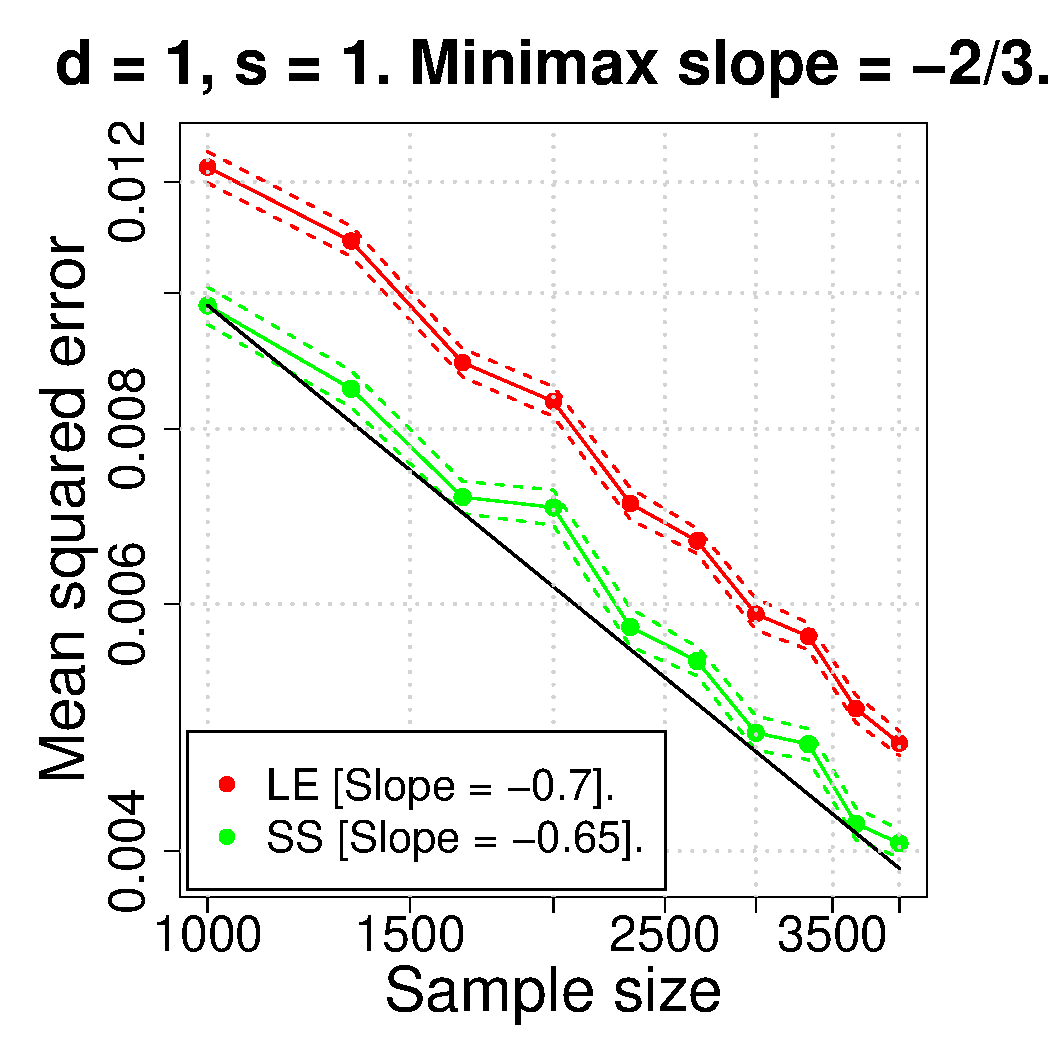
\includegraphics[width=.245\textwidth]{../figures/mse/mse_by_sample_size_1d_1s.pdf}
	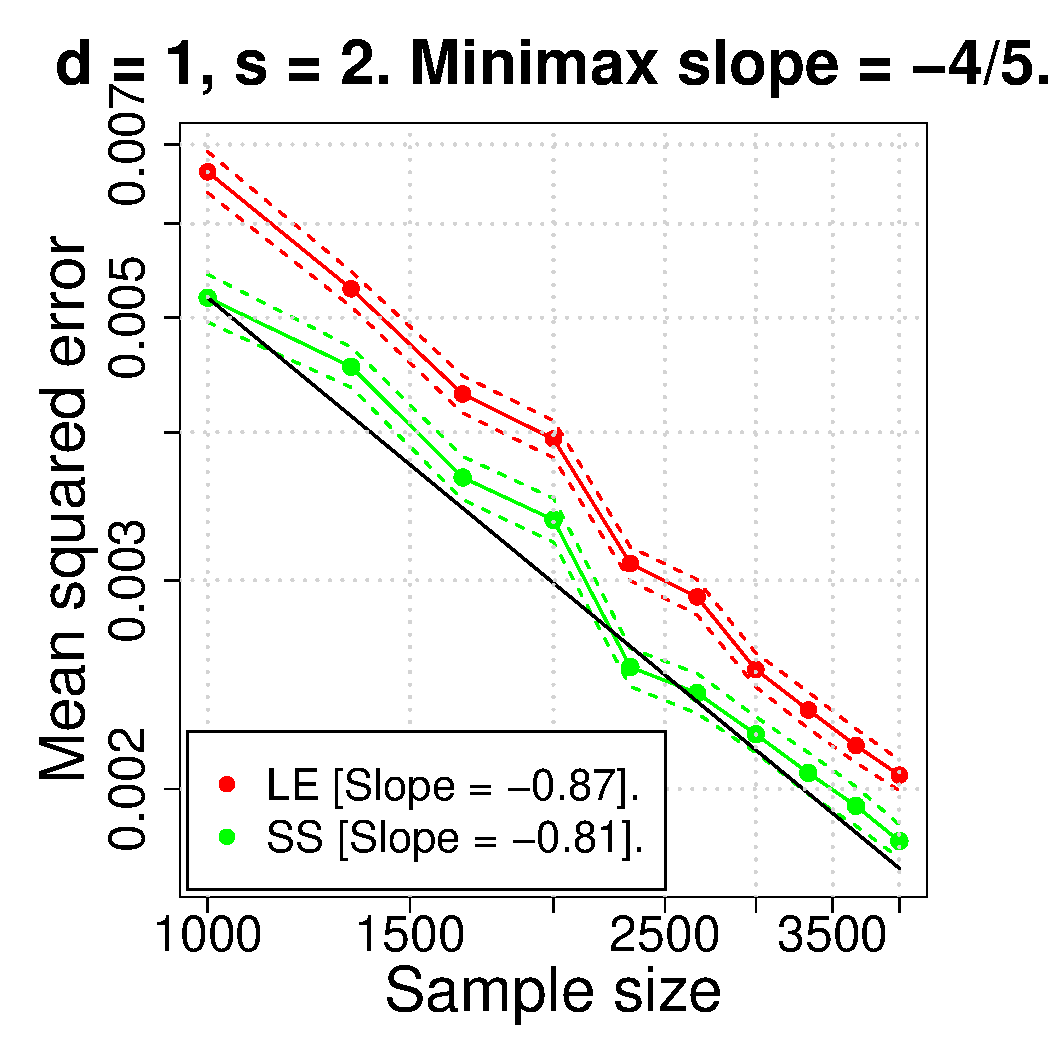
\includegraphics[width=.245\textwidth]{../figures/mse/mse_by_sample_size_1d_2s.pdf}
	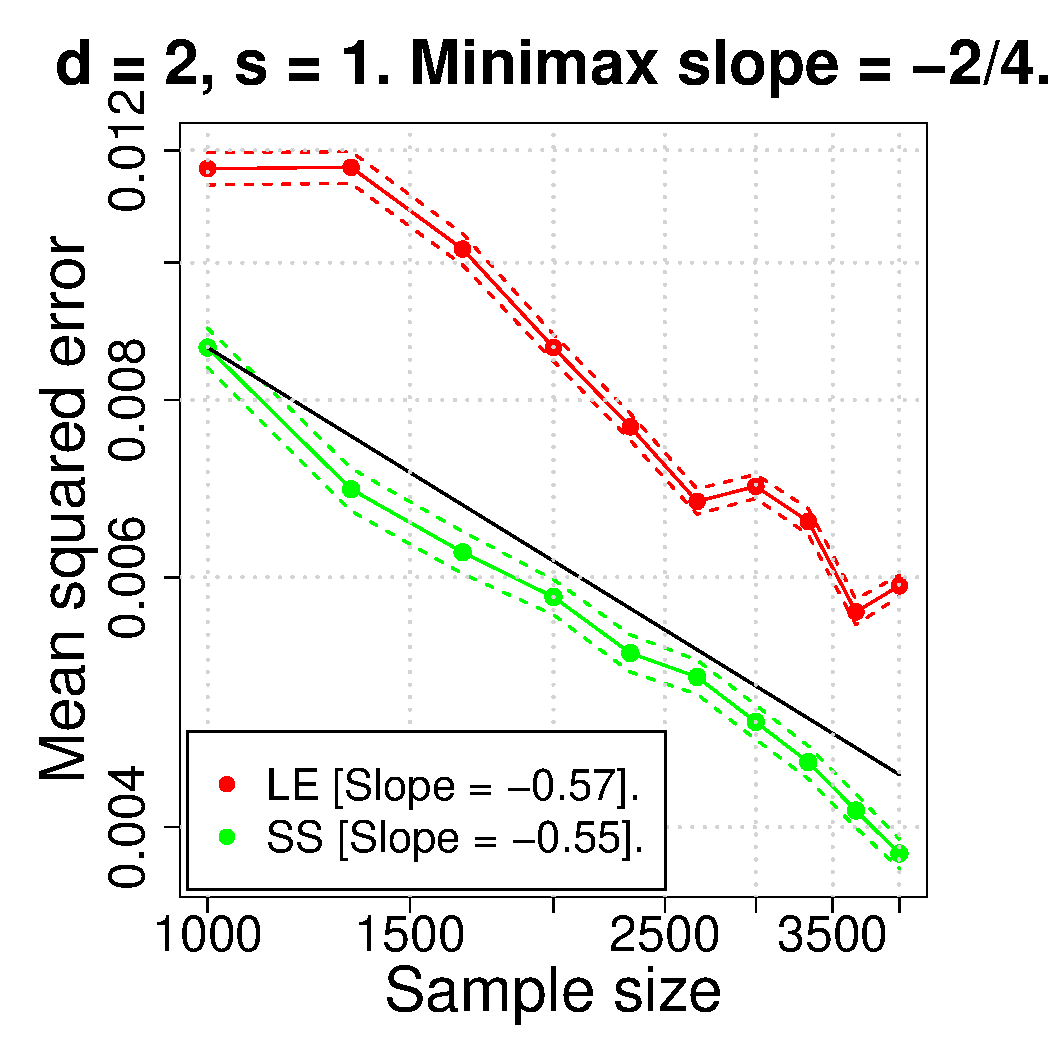
\includegraphics[width=.245\textwidth]{../figures/mse/mse_by_sample_size_2d_1s.pdf}
	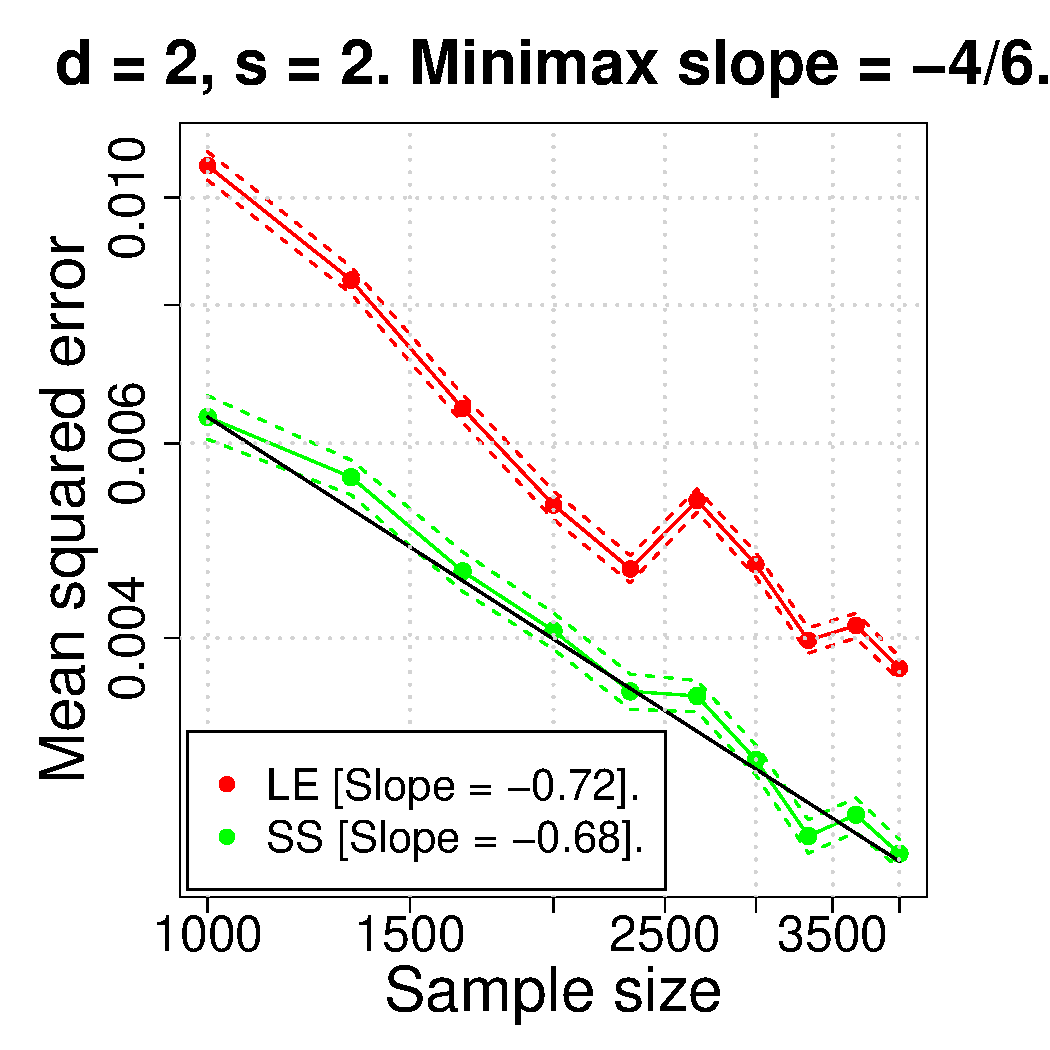
\includegraphics[width=.245\textwidth]{../figures/mse/mse_by_sample_size_2d_2s.pdf}
	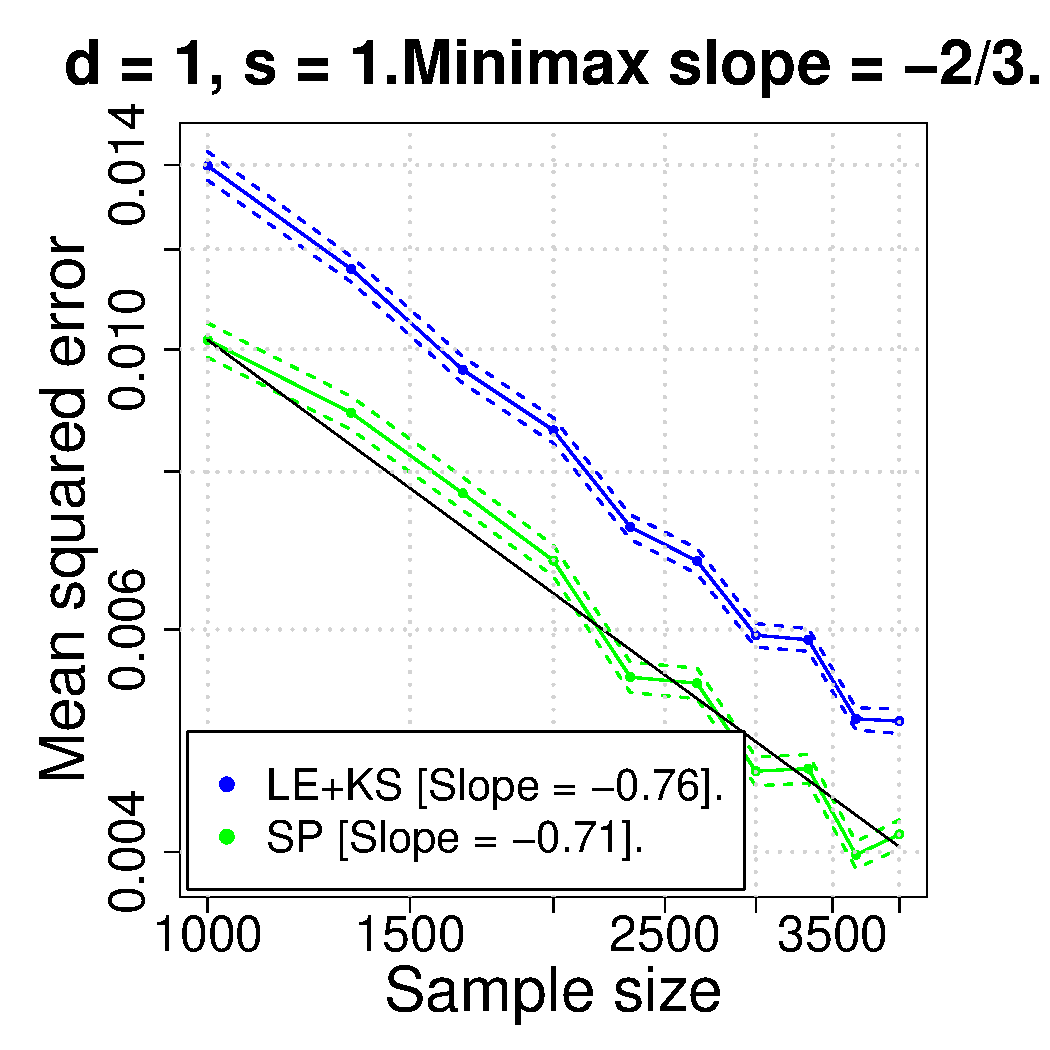
\includegraphics[width=.245\textwidth]{../figures/out_of_sample_mse/mse_by_sample_size_1d_1s.pdf}
	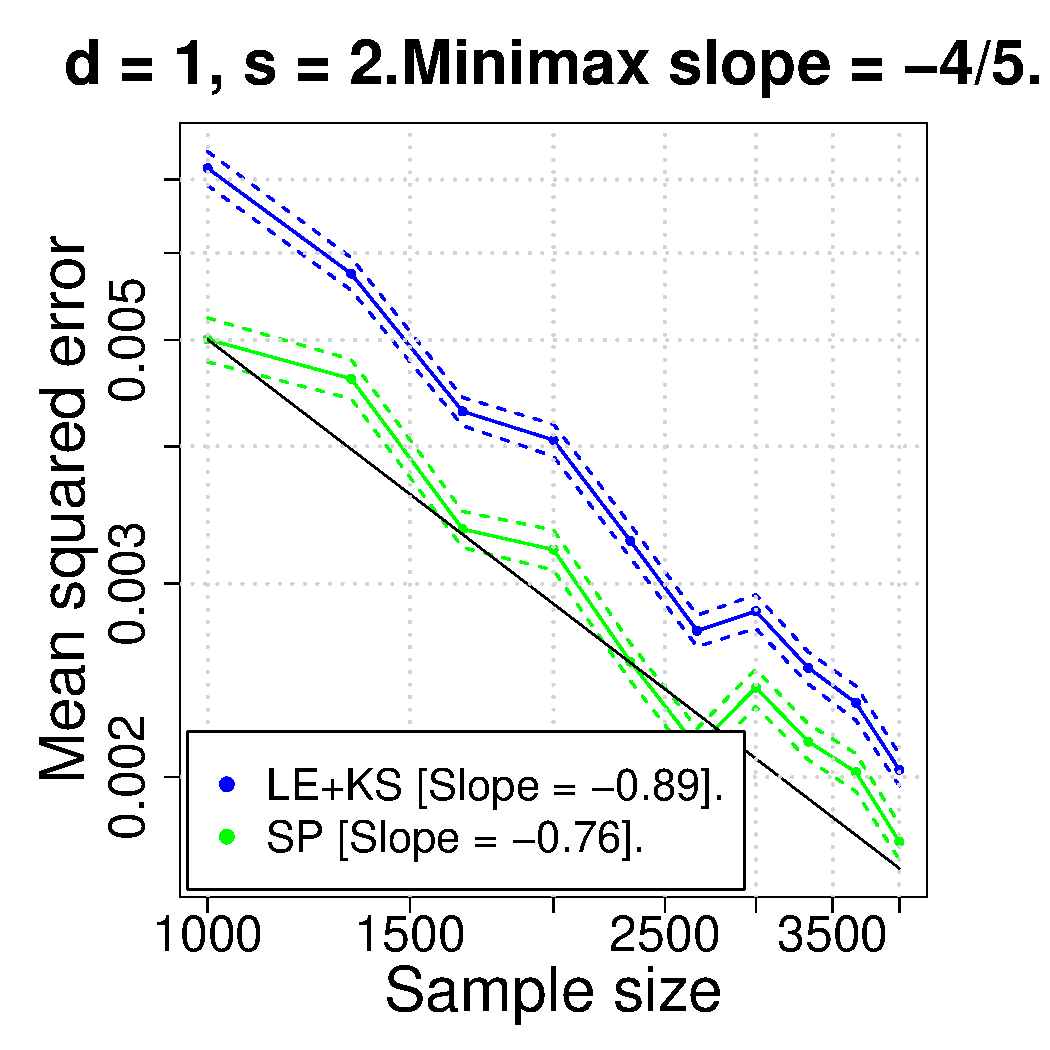
\includegraphics[width=.245\textwidth]{../figures/out_of_sample_mse/mse_by_sample_size_1d_2s.pdf}
	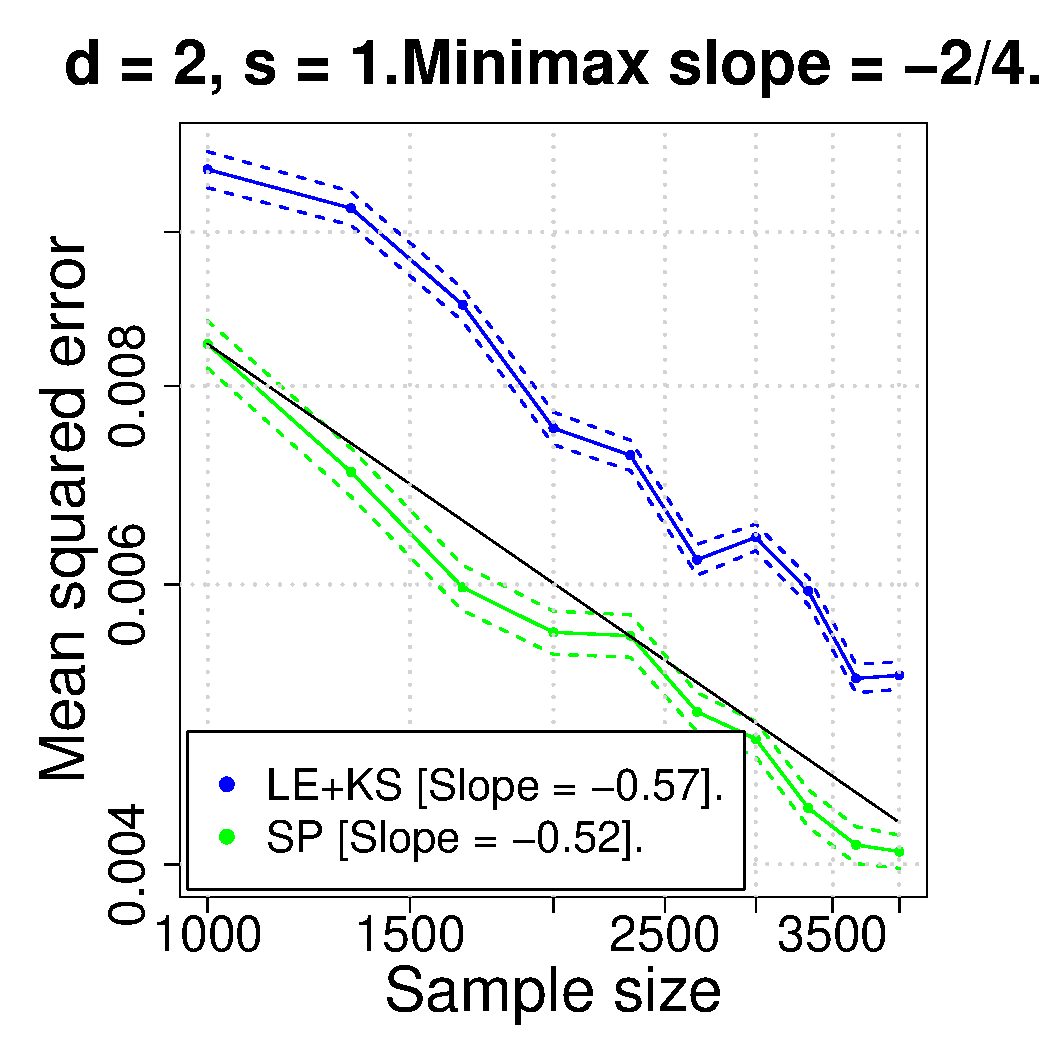
\includegraphics[width=.245\textwidth]{../figures/out_of_sample_mse/mse_by_sample_size_2d_1s.pdf}
	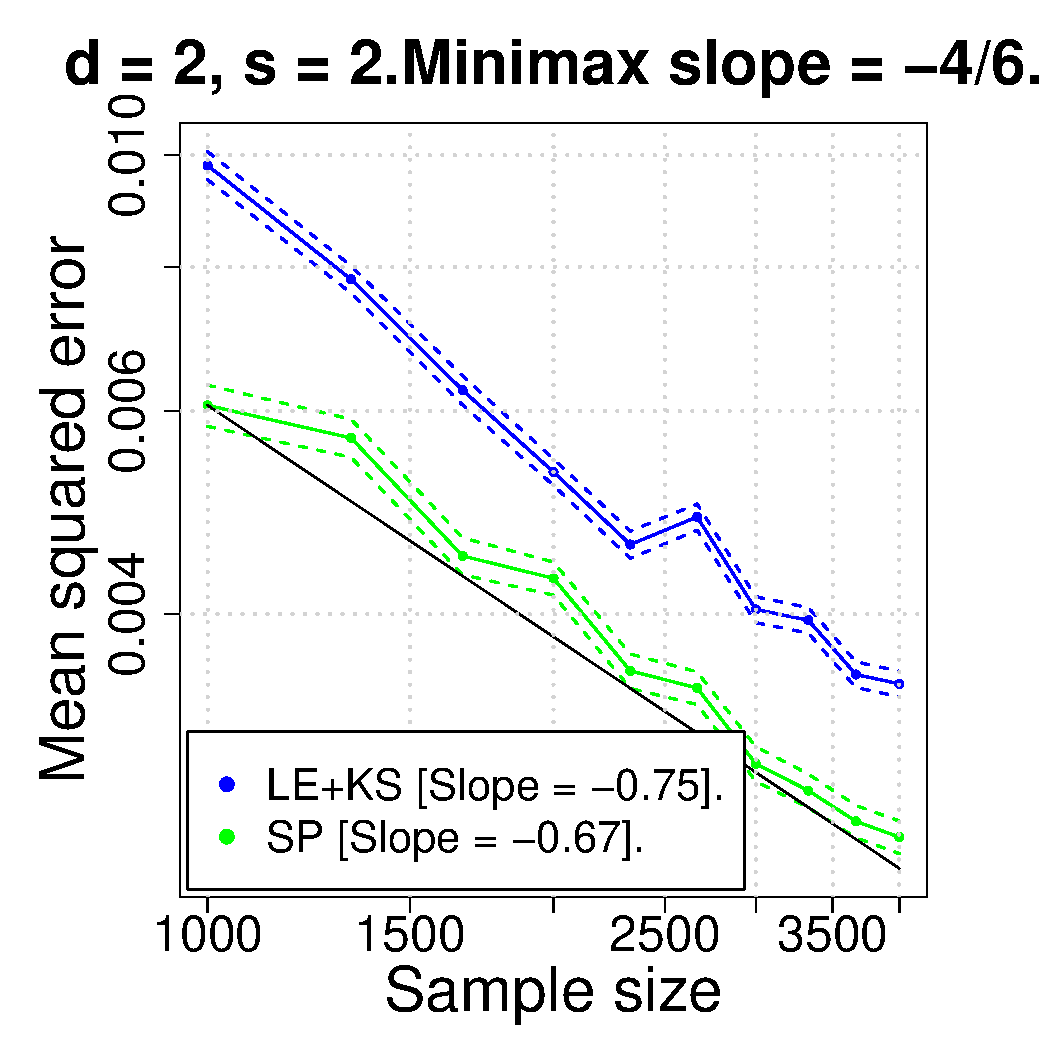
\includegraphics[width=.245\textwidth]{../figures/out_of_sample_mse/mse_by_sample_size_2d_2s.pdf}
	\caption{Mean squared error (mse) of Laplacian eigenmaps and spectral projection estimators. Top row: in-sample mse of Laplacian eigenmaps (\texttt{LE}) and a spectral projection estimator (\texttt{SP}) as a function of sample size $n$. Bottom row: out-of-sample mse of Laplacian eigenmaps plus kernel smoothing (\texttt{LE+KS}) and a spectral projection estimator. Each plot is on the log-log scale, and the results are averaged over 400 repetitions. All estimators are tuned for optimal average mse. The black line shows the minimax rate (in slope only; the intercept is chosen to match the observed error).}
	\label{fig:fig1}
\end{figure*}

\subsection{Estimation}
In our first experiment, we compare the mean-squared error of the Laplacian eigenmaps estimator $\wh{f}$  to that of its population-level counterpart $\wt{f}$. We vary the sample size from $n = 1000$ to $n = 4000$; sample $n$ design points $\{X_1,\ldots,X_n\}$ from the uniform distribution on the cube $[-1,1]^d$; and sample responses $Y_i$ according to~\eqref{eqn:model} with regression function $f_0 = M/\lambda_K^{s/2} \cdot \psi_K$ for $K \asymp n^{d/(2s + d)}$ (the pre-factor $M/\lambda_K^{s/2}$ is chosen so that $|f_0|_{H^s(\mc{X})}^2 = M^2$). In Figure~\ref{fig:fig1} we show the in-sample mean-squared error of the two estimators as a function of $n$, for different dimensions $d$ and order of smoothness $s$. We see that all estimators have mean-squared error converging to zero at roughly the minimax rate. While unsurprisingly population-level spectral projection has smaller error, generally speaking the error of Laplacian eigenmaps approaches that of population-level spectral projection as $n$ gets larger. 

We also compare the out-of-sample estimation error, over a held-out test set, of Laplacian eigenmaps plus kernel smoothing to the spectral projection estimator. The story is much the same, supporting our theoretical claim that the additional error incurred by kernel smoothing of Laplacian eigenmaps is negligible.

\subsection{Testing} 
In our second experiment, we compare the Laplacian eigenmaps test $\varphi$ against the  population-level spectral projection test $\wt{\varphi}$. The setup is generally the same as that of our first experiment, but to get an empirical estimate of the critical radius the details are necessarily somewhat more complicated. First we take $\mc{F} = \{M/\lambda_k^{s/2} \psi_k\}_{k = 1}^{n}$ to be a discrete subset of $H^1(\mc{X};M)$. Then, for each $f_0 \in \mc{F}$, we run a given test $\phi$ (either the Laplacian eigenmaps test $\phi = \varphi$, or the population-level spectral projection test $\phi = \wt{\varphi}$.) and record whether it was a false negative or true positive. We repeat this process over $100$ replications, giving a Monte Carlo estimate of the type II error $E_{f_0}[1 - \phi]$ for each $f_0 \in \mc{F}$. Finally, we take the smallest value of $\|f_0\|_P^2$ such $E_{f_0}[1 - \phi] \leq b$ as our estimate of the critical radius of $\phi$. 

In Figure~\ref{fig:fig2}, we see that the estimated critical radii of both Laplacian eigenmaps and population-level spectral projection tests are quite close to each other, and converge at roughly the minimax rate.
\begin{figure*}[tb]
	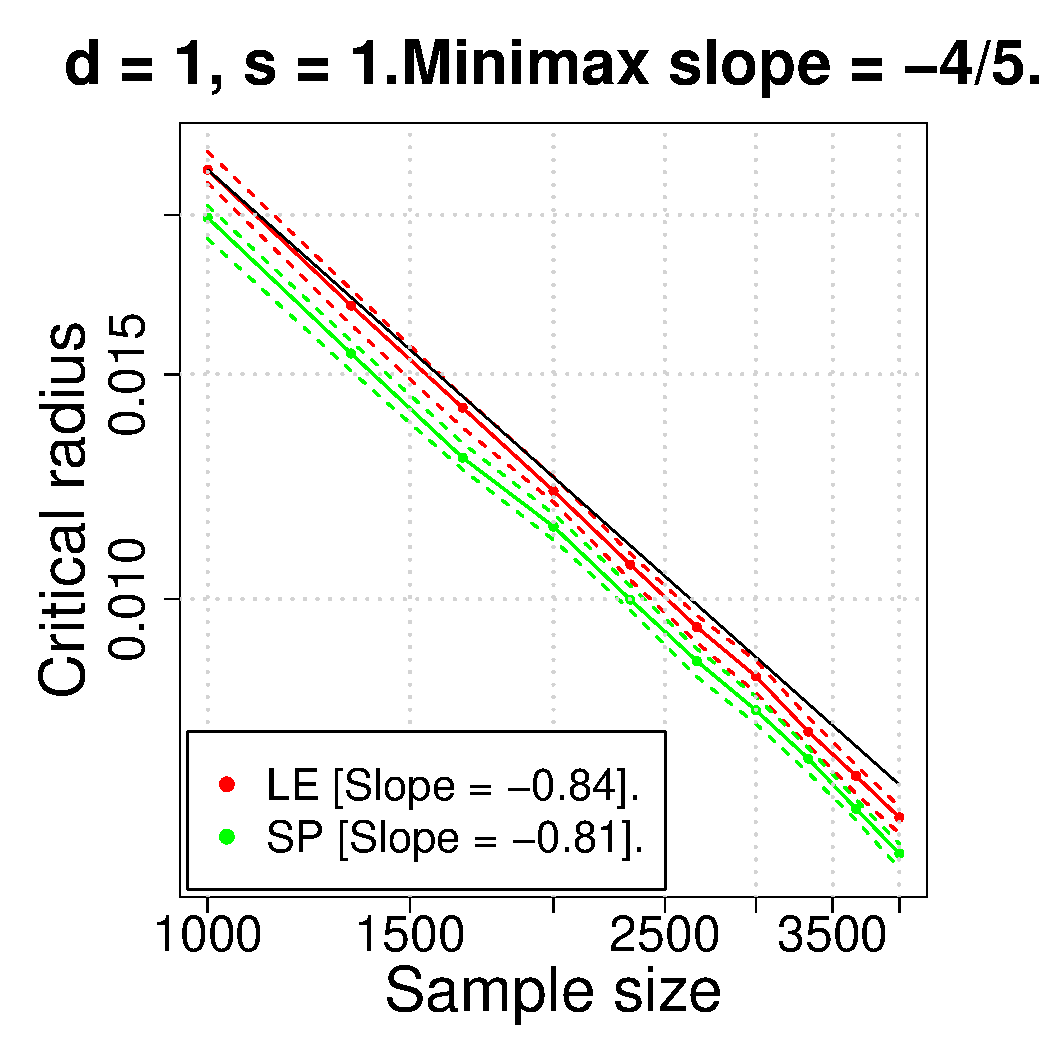
\includegraphics[width=.245\textwidth]{../figures/testing/eigenfunction/critical_radius_by_sample_size_1d_1s.pdf}
	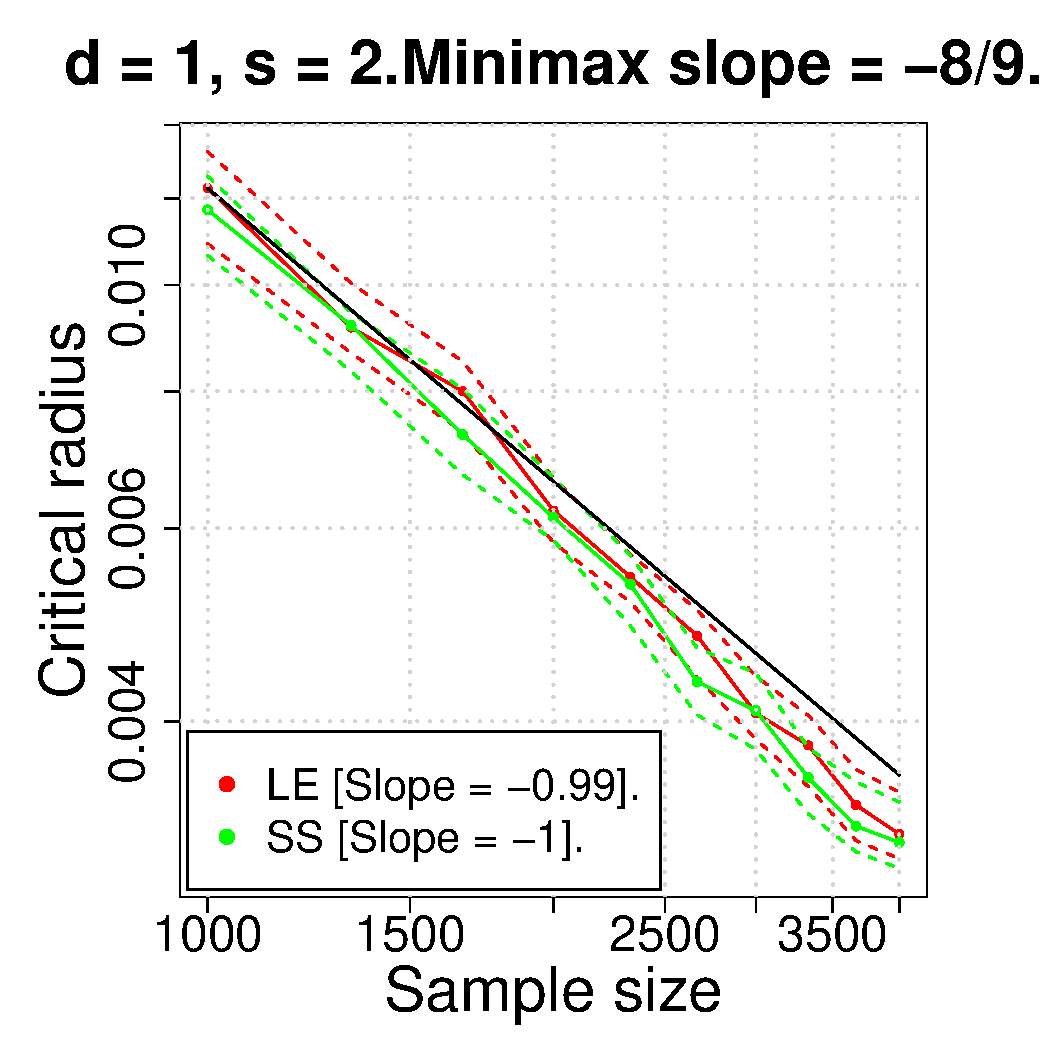
\includegraphics[width=.245\textwidth]{../figures/testing/eigenfunction/critical_radius_by_sample_size_1d_2s.pdf}
	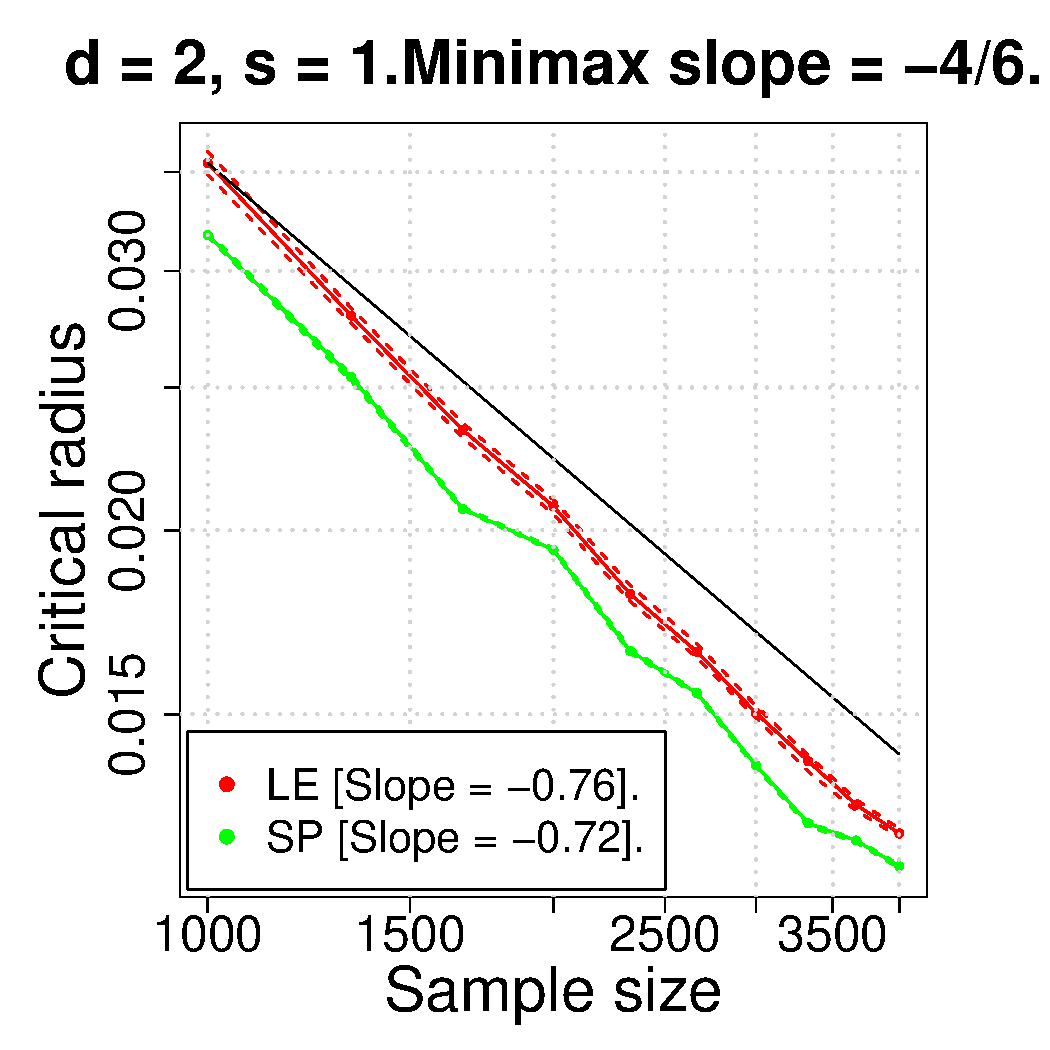
\includegraphics[width=.245\textwidth]{../figures/testing/eigenfunction/critical_radius_by_sample_size_2d_1s.pdf}
	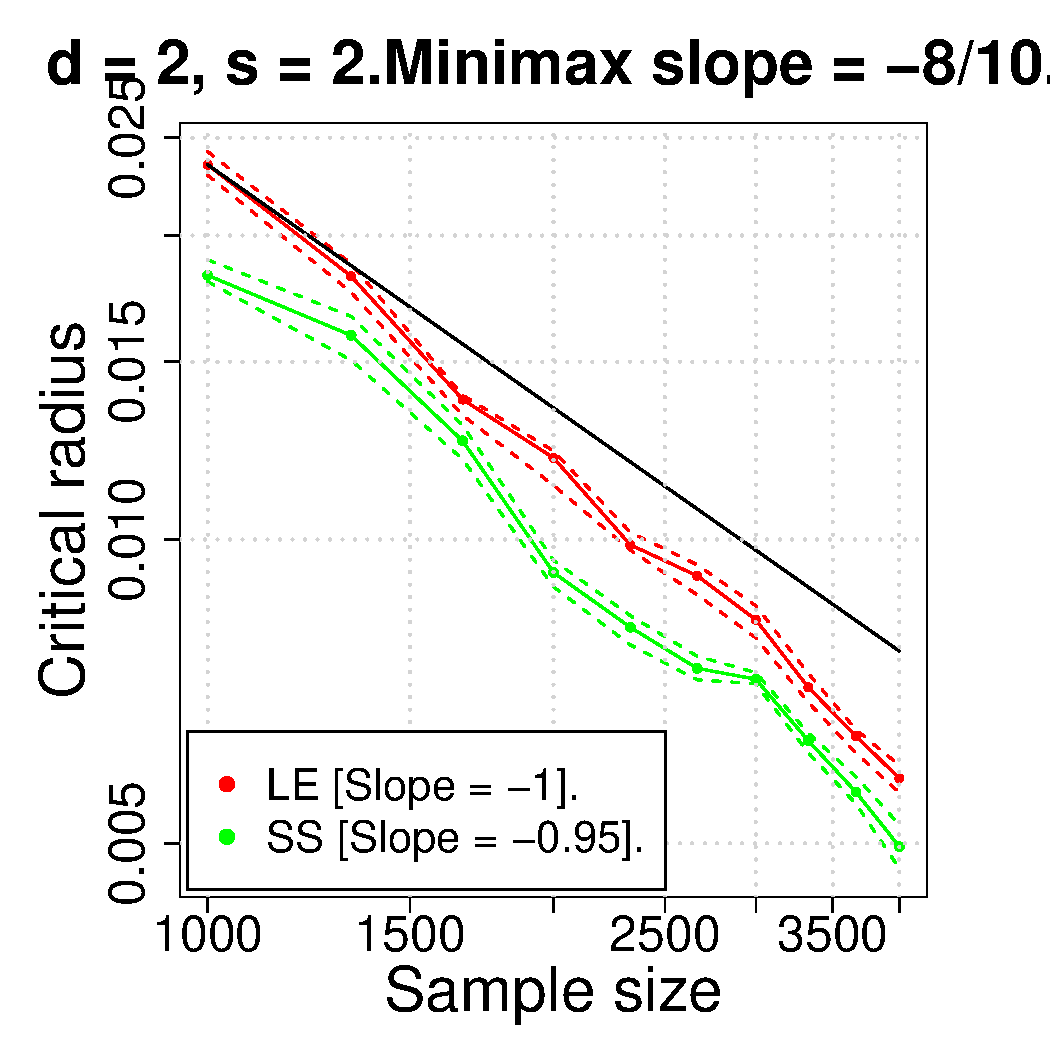
\includegraphics[width=.245\textwidth]{../figures/testing/eigenfunction/critical_radius_by_sample_size_2d_2s.pdf}
	\caption{Worst-case testing risk Laplacian eigenmaps (\texttt{LE}) and spectral projection (\texttt{SP}) tests, as a function of sample size $n$. Plots are on the same scale as Figure~\ref{fig:fig1}, and black line shows the minimax rate. All tests are set to have $.05$ Type I error, and are calibrated by simulation under the null.}
	\label{fig:fig2}
\end{figure*}

\subsection{Tuning parameters}
Our first two experiments demonstrate that Laplacian eigenmaps methods have comparable statistical performance to spectral projection methods. Laplacian eigenmaps depends on two tuning parameters, and in our final experiment we investigate the importance of both, focusing now on estimation. In Figure~\ref{fig:fig3}, we see how the mean-squared error of Laplacian eigenmaps changes as each tuning parameter is varied. As suggested by our theory, properly choosing the number of eigenvectors $K$ is crucial: the mean-squared error curves, as a function of $K$, always have a sharply defined minimum. On the other hand, as a function of the graph radius parameter $\varepsilon$ the mean-squared error curve is much closer to flat. This squares completely with our theory, which requires that the number of eigenvectors $K$ be much more carefully tuned that the graph radius $\varepsilon$.

We also plot the out-of-sample mean squared error of Laplacian eigenmaps plus kernel smoothing, as a function of its various tuning parameters (which include the bandwidth $h$ as well as $\varepsilon$ and $K$.) Here the relationship between theory and empirics is more nuanced. On the one hand, empirically it seems that the optimal choice of bandwidth parameter $h$ is usually smaller than $\varepsilon$, as suggested by our theory. On the other hand, for Laplacian eigenmaps plus kernel smoothing we see that as a function of $K$, the mean-squared error curves are close to their minima even when we choose many more eigenvectors than is optimal for Laplacian eigenmaps. This is not reflected in our theory, which requires that $K$ be chosen in the same tight range as was required for Laplacian eigenmaps to be optimal in-sample. However, it does make intuitive sense: extension by kernel smoothing further attenuates the noise, making the algorithm more forgiving to overfitting during the Laplacian eigenmaps step. 

\begin{figure*}[tb]
	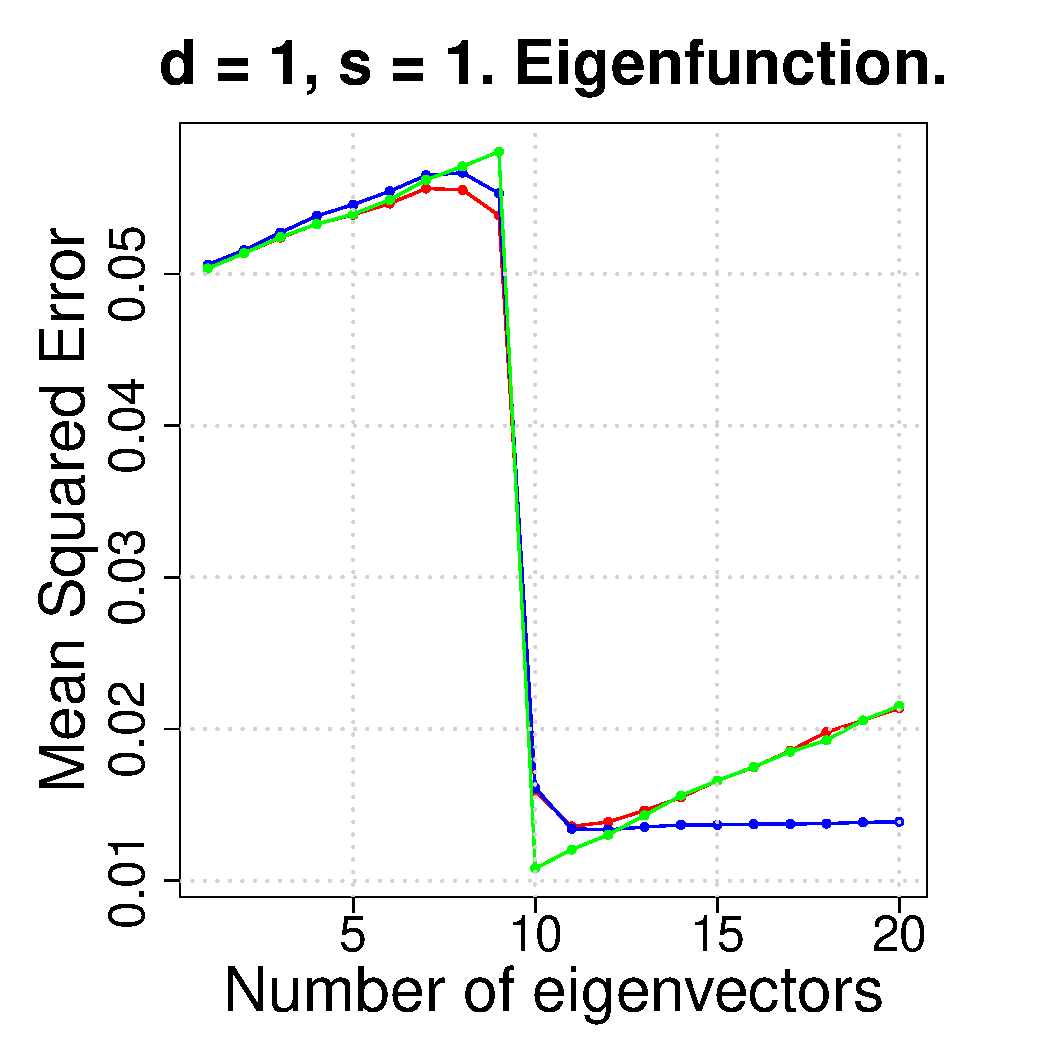
\includegraphics[width=.245\textwidth]{../figures/tuning/eigenfunction/mse_by_number_of_eigenvectors_1d_1s.pdf}
	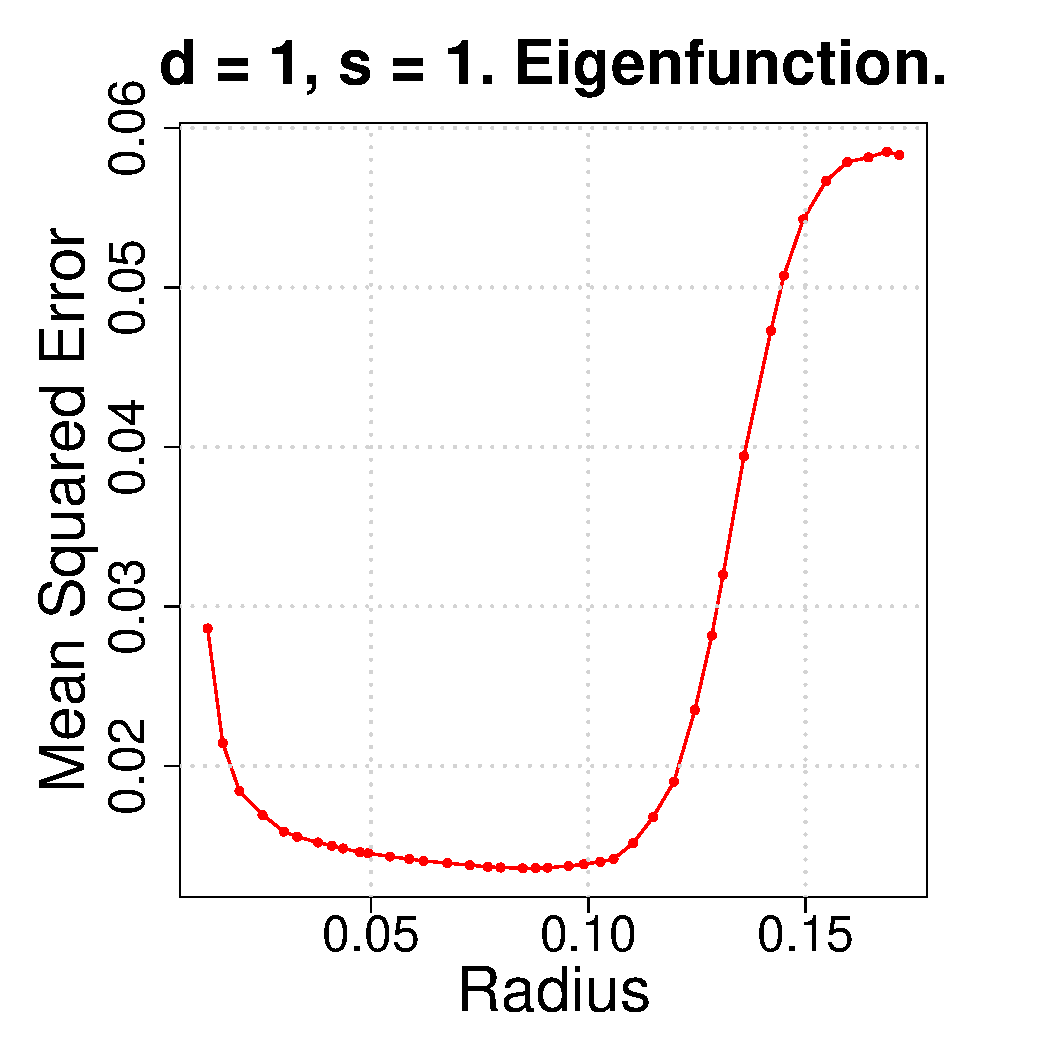
\includegraphics[width=.245\textwidth]{../figures/tuning/eigenfunction/mse_by_radius_1d_1s.pdf} 
	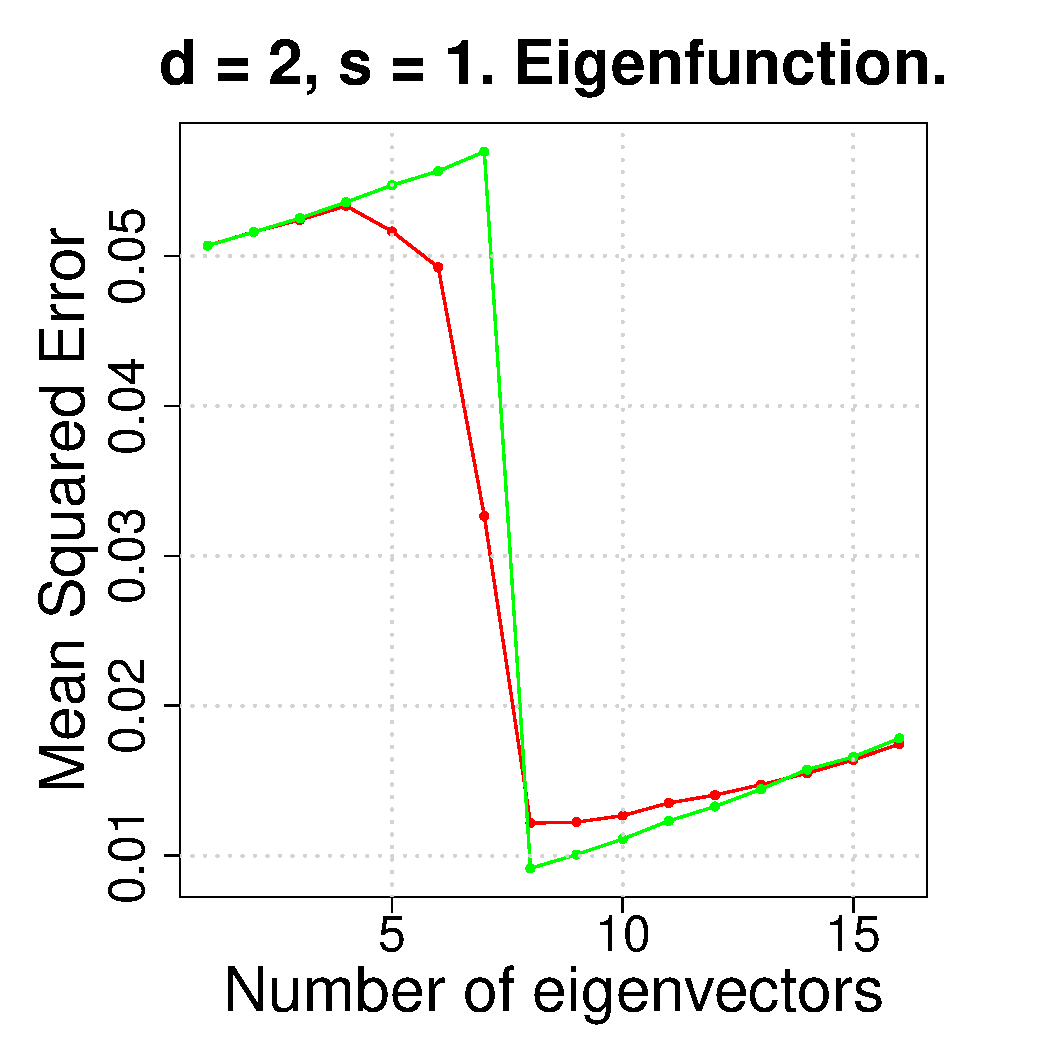
\includegraphics[width=.245\textwidth]{../figures/tuning/eigenfunction/mse_by_number_of_eigenvectors_2d_1s.pdf}
	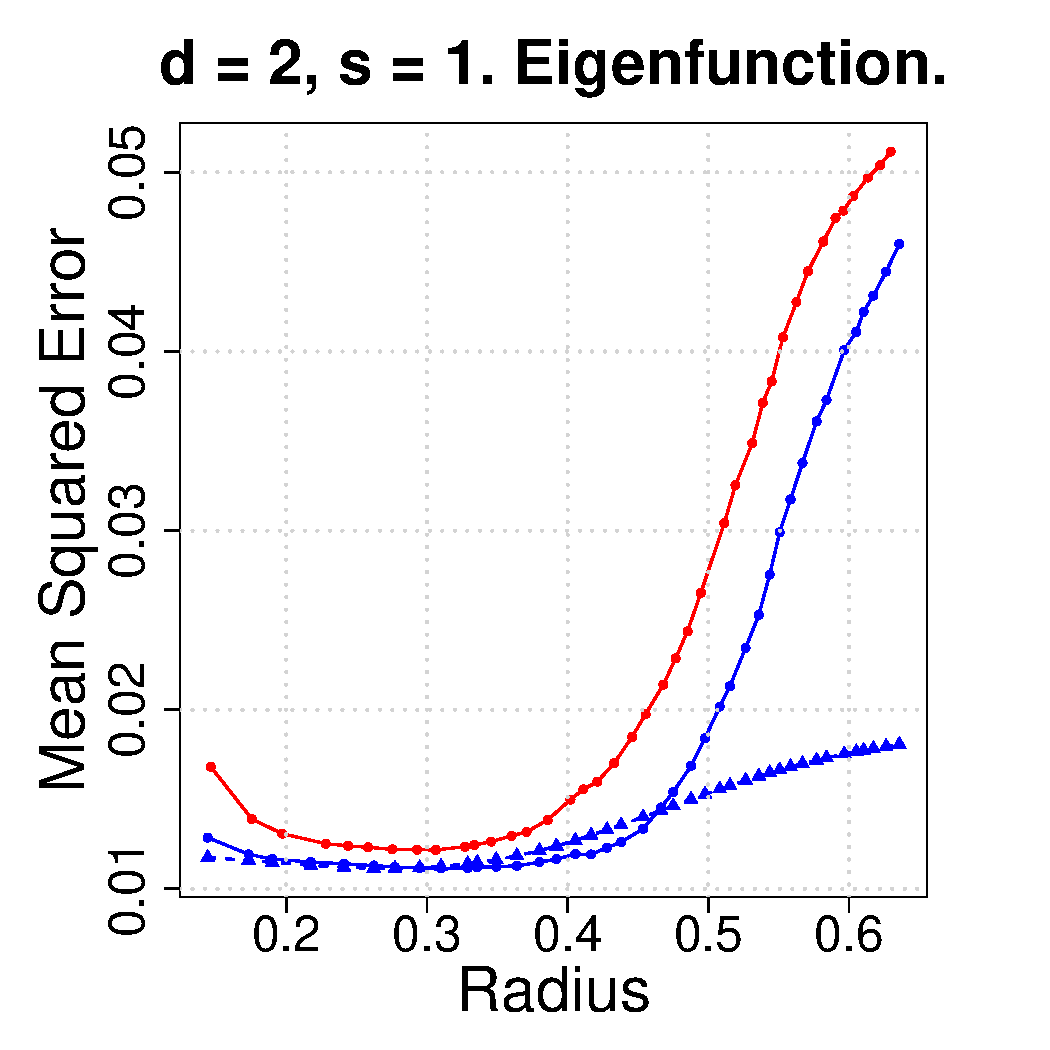
\includegraphics[width=.245\textwidth]{../figures/tuning/eigenfunction/mse_by_radius_2d_1s.pdf} 
	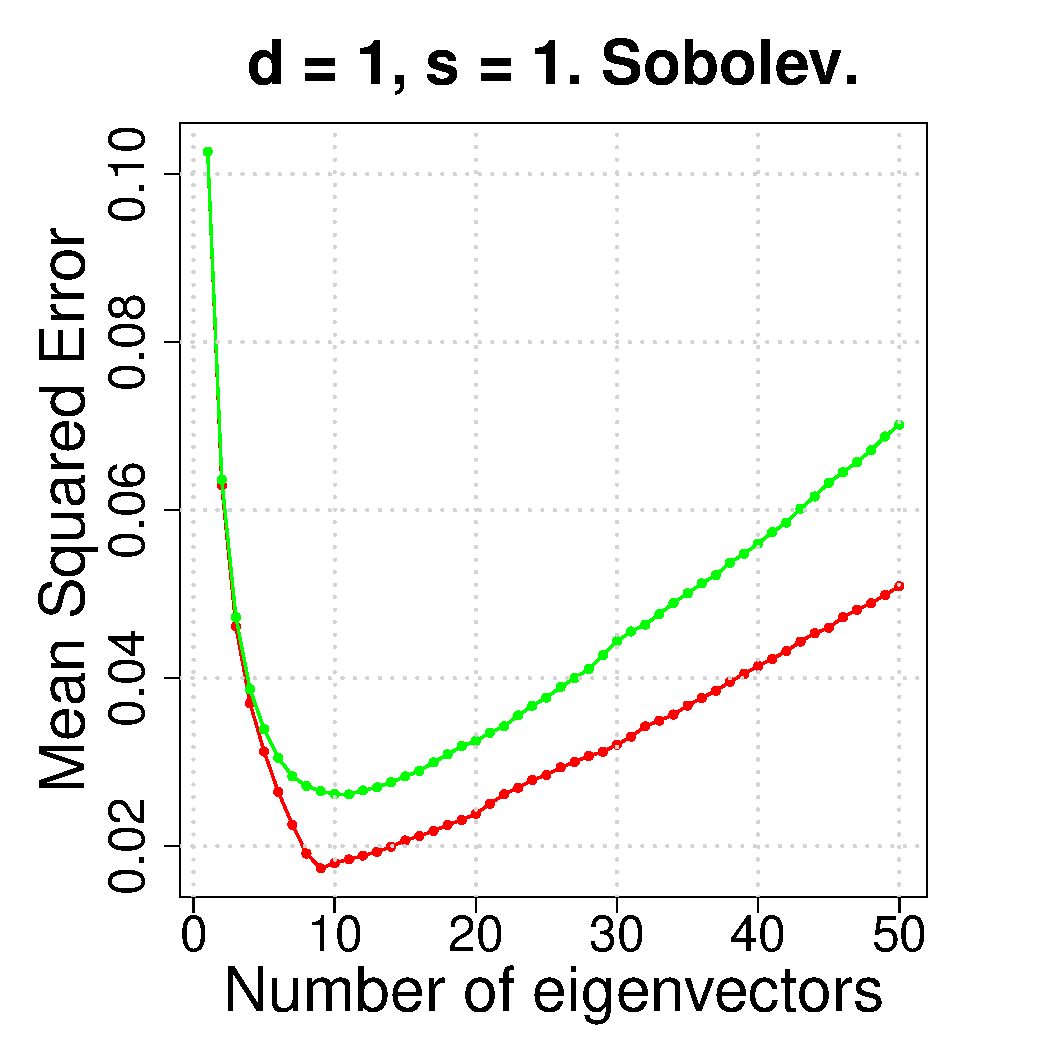
\includegraphics[width=.245\textwidth]{../figures/tuning/sobolev/mse_by_number_of_eigenvectors_1d_1s.pdf}
	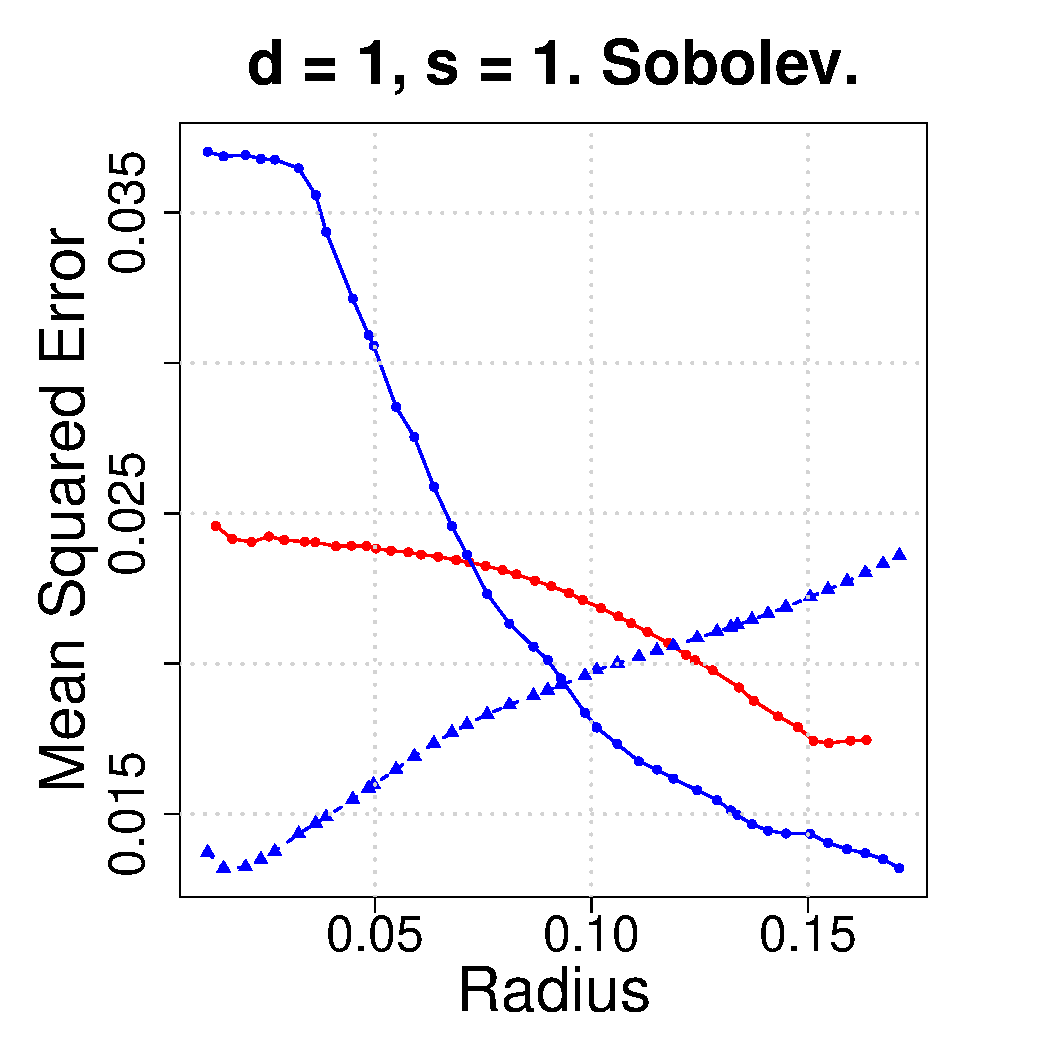
\includegraphics[width=.245\textwidth]{../figures/tuning/sobolev/mse_by_radius_1d_1s.pdf}
	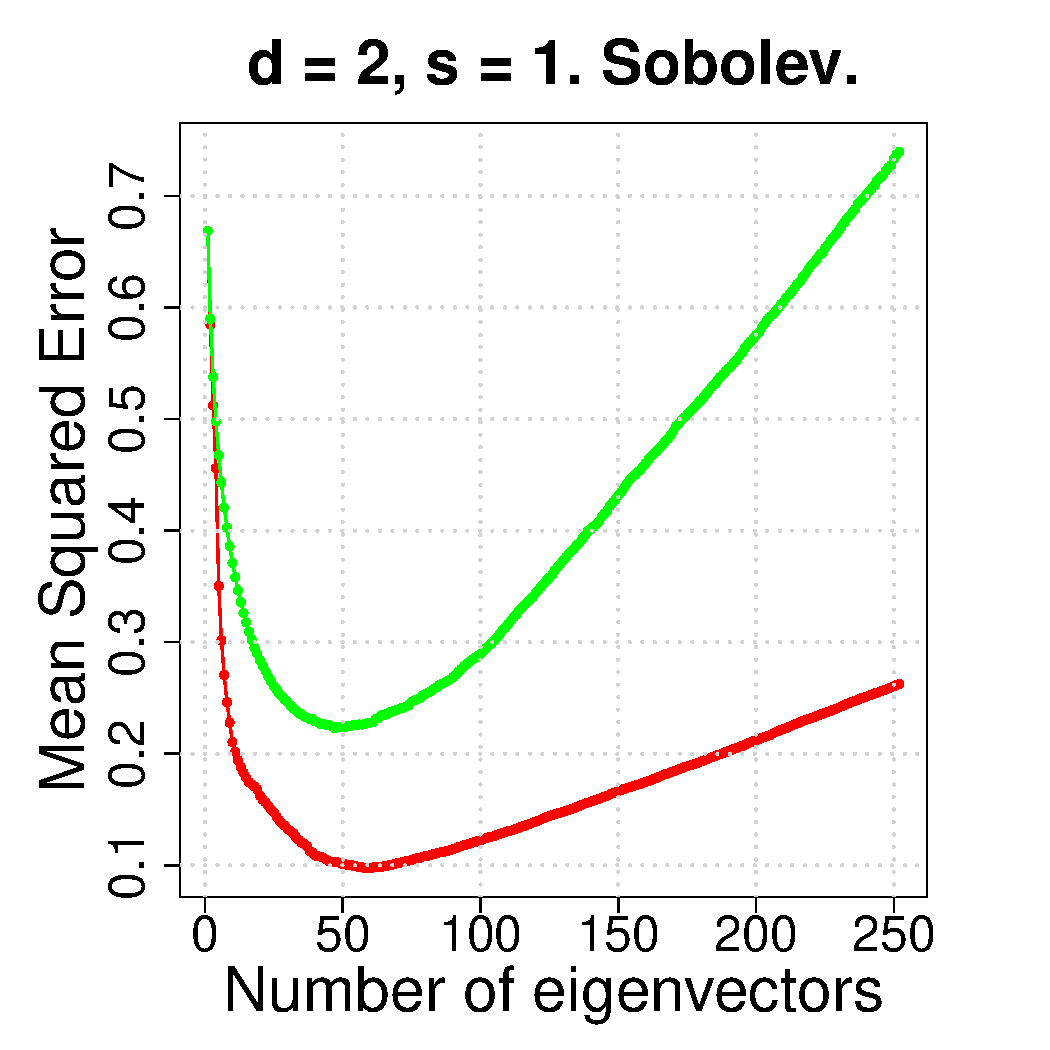
\includegraphics[width=.245\textwidth]{../figures/tuning/sobolev/mse_by_number_of_eigenvectors_2d_1s.pdf}
	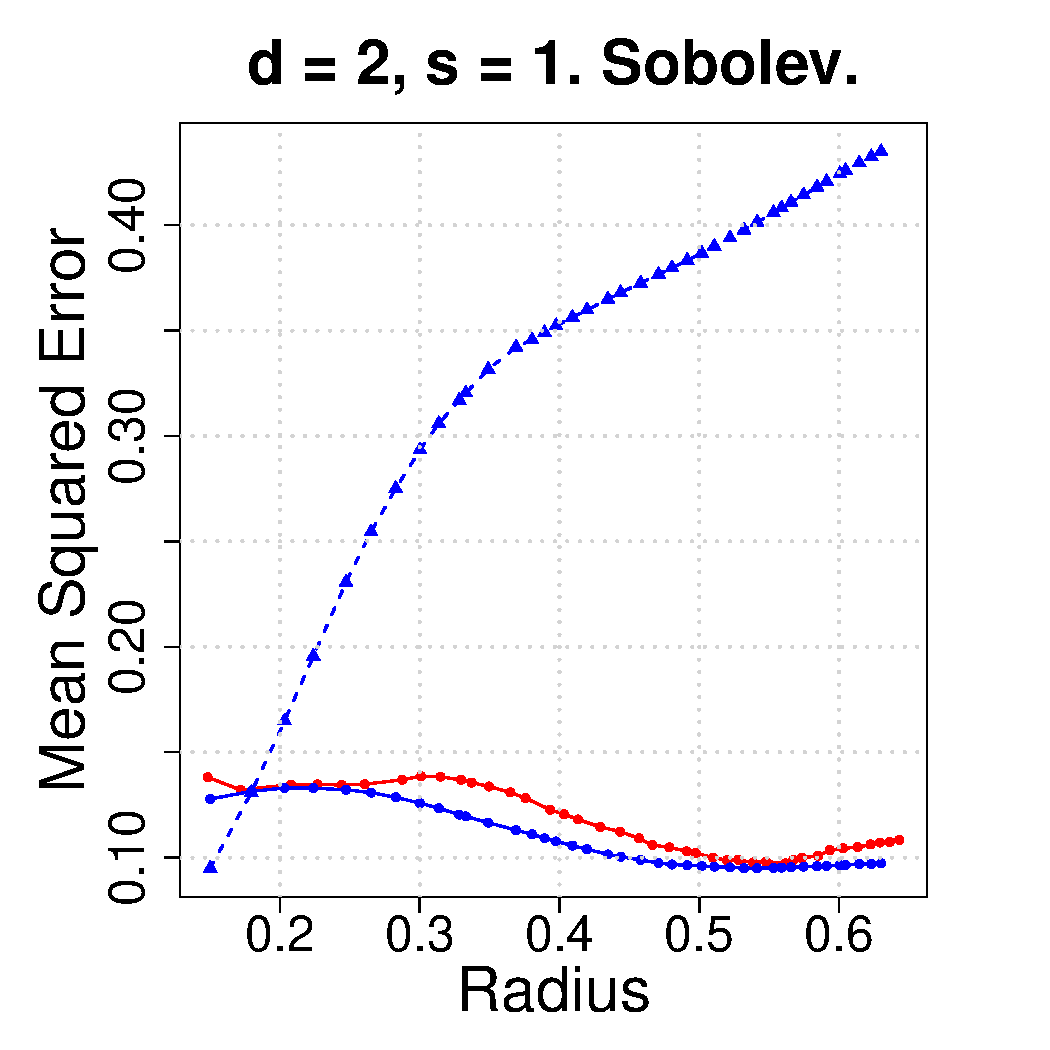
\includegraphics[width=.245\textwidth]{../figures/tuning/sobolev/mse_by_radius_2d_1s.pdf}  
	\caption{Mean squared error of Laplacian eigenmaps (\textcolor{red}{red}), Laplacian eigenmaps plus kernel smoothing (\textcolor{blue}{blue}), and spectral projection (\textcolor{green}{green}) as a function of tuning parameters. Top row: the same regression function $f_0$ as used in Figure~\ref{fig:fig1}. Bottom row: the regression function $f_0 \propto \sum_{k} 1/\lambda_k^{1/2} \psi_k$. For all experiments, the sample size $n = 1000$, and the results are averaged over $200$ repetitions. In each panel, all tuning parameters except the one being varied are set to their optimal values. For Laplacian eigenmaps plus kernel smoothing, circular points and a solid line are used to denote the error as a function of the graph radius $\varepsilon$, whereas triangular points and a dashed line are used to denote the error as a function of the bandwidth $h$.}
	\label{fig:fig3}
\end{figure*}

\section{Discussion}
\label{sec:discussion}

In this work, we have derived upper bounds on the rates of convergence for methods based on Laplacian eigenmaps, which imply that in various settings these methods are minimax rate-optimal over Sobolev classes. Importantly, these upper bounds hold under nonparametric conditions on the design density $p$, and allow for $p$ to be unknown and, potentially, supported on a low-dimensional manifold. Our results help explain the practical success of methods which leverage graph Laplacian eigenvectors for regression. They also distinguish Laplacian eigenmaps from more traditional spectral projection procedures, which rely on a density-dependent basis and thus require the density be known a priori.

Of course, there do exist other methods for nonparametric regression which achieve optimal rates of convergence under similar (or indeed weaker) conditions on $p$. These include other graph-based approaches---graph Laplacian regularization---methods besides spectral projection---e.g. kernel smoothing, local polynomial regression, thin-plate splines---and continuum spectral projection methods which use the eigenfunctions of an operator defined independently of $p$. To be clear, we do not advocate Laplacian eigenmaps over these alternatives. Rather, we view our results as theoretically justifying a place for Laplacian eigenmaps in the nonparametric regression toolbox. 

That being said, Laplacian eigenmaps does have certain advantages over each of the aforementioned approaches. We now conclude by outlining some of these advantages (limiting our discussion to estimation):
\begin{itemize}
	\item \emph{Optimality over high-dimensional Sobolev spaces}. Graph Laplacian regularization achieves minimax optimal rates over $H^1(\mc{X})$ only when $d \in \{1,2,3,4\}$ \citep{sadhanala16, green2021}; when $d \geq 5$, graph Laplacian regularization appears to be suboptimal. In contrast, Laplacian eigenmaps is optimal over $H^1(\mc{X})$ for all dimensions $d$.  An even more stark contrast can be drawn between Laplacian eigenmaps (and other spectral projection estimators) and the first order thin-plate spline, the solution of the variational problem
	\begin{equation}
	\underset{f \in H^1(\mc{X})}{\textrm{minimize}} \quad  \|{\bf Y} - f\|_n^2 + \lambda \|f\|_{H^1(\Reals^d)}^2,
	\end{equation}
	which is optimal and indeed well-posed only when $d = 1$. This appears to be related to a general phenomenon described by~\cite{dhillon2013,dicker2017}, in which principal components analysis followed by ordinary least-squares is shown to be always competitive with, and sometimes much better than, ridge regression. 
	\item \emph{Manifold adaptivity}. An oft-recommended alternative to the population-level spectral projection methods considered in Section~\ref{subsec:spectral_projection} is to run ordinary least-squares regression using eigenfunctions of a density-independent operator, such as the Laplacian $\Delta = \sum_{i = 1}^{d} \partial^2f/\partial x_i^2$. Under the conditions of Model~\ref{def:model_flat_euclidean}, such a method will indeed be rate-optimal, though the upper bounds may come with undesirably large constants if $p$ is very non-uniform. However, in contrast with Laplacian eigenmaps, under Model~\ref{def:model_manifold} this method cannot achieve the faster minimax rates of convergence.
	\item \emph{Density adaptivity}. It is natural to ask whether the two stage estimator $T_{n,h}\wh{f}$ defined in Section~\ref{sec:out_of_sample} has any advantage over the simpler approach of directly kernel smoothing the responses, i.e. using the estimator $T_{n,h}{\bf Y}$ (possibly for a different choice of $h$). In Appendix~F.4 of the Supplementary Material, we answer this question in the affirmative, by giving a simple example of a sequence of densities and regression functions $\{(p^{(n)}, f_0^{(n)}: n \in \mathbb{N}\}$ such that $\Ebb\|f_0 - T_{n,h}\wh{f}\|_P^2$ is of a strictly lower order than $\inf_{h'} \Ebb\|f_0 - T_{n,h'}{\bf Y}\|_P^2$. This is possible because Laplacian eigenmaps induces a completely different bias than kernel smoothing. For example, when $f_0$ and $p$ satisfy the so-called \emph{cluster assumption}---meaning $f_0$ is piecewise constant in high-density regions (clusters) of $p$---then the bias of Laplacian eigenmaps can be much smaller than that of kernel smoothing (for equivalent levels of variance). 
	
	We emphasize that this does not contradict the well-known optimality properties of kernel smoothing over e.g. H\"{o}lder balls. Rather, in the standard nonparametric regression setup---which we adopt in the main part of this paper, and in which $P$ is assumed to be equivalent to Lebesgue measure---the biases of Laplacian eigenmaps and kernel smoothing happen to be equivalent. But when $P$ is sufficiently non-uniform, this is no longer the case.
\end{itemize}
Grounding each of these three points on a firmer and more complete theoretical basis would be, in our view, a valuable direction for future work.

%%%%%%%%%%%%%%%%%%%%%%%%%%%%%%%%%%%%%%%%%%%%%%
%% Support information, if any,             %%
%% should be provided in the                %%
%% Acknowledgements section.                %%
%%%%%%%%%%%%%%%%%%%%%%%%%%%%%%%%%%%%%%%%%%%%%%
%\begin{acks}[Acknowledgments]
%
%\end{acks}
%%%%%%%%%%%%%%%%%%%%%%%%%%%%%%%%%%%%%%%%%%%%%%
%% Funding information, if any,             %%
%% should be provided in the                %%
%% funding section.                         %%
%%%%%%%%%%%%%%%%%%%%%%%%%%%%%%%%%%%%%%%%%%%%%%
%\begin{funding}
%\end{funding}

%%%%%%%%%%%%%%%%%%%%%%%%%%%%%%%%%%%%%%%%%%%%%%
%% Supplementary Material, including data   %%
%% sets and code, should be provided in     %%
%% {supplement} environment with title      %%
%% and short description. It cannot be      %%
%% available exclusively as external link.  %%
%% All Supplementary Material must be       %%
%% available to the reader on Project       %%
%% Euclid with the published article.       %%
%%%%%%%%%%%%%%%%%%%%%%%%%%%%%%%%%%%%%%%%%%%%%%
\begin{supplement}
\stitle{Supplement to ``Minimax-Optimal Regression Over Sobolev Spaces via Laplacian Eigenmaps with Neighborhood Graphs''.}
\sdescription{The supplement contains all proofs omitted from the main text due to space constraints.}
\end{supplement}

% Bibliography
\bibliographystyle{imsart-nameyear}
\bibliography{../../../graph_regression_bibliography}

\end{document}
